
% Copyright (C) 2014-2017 by Thomas Auzinger <thomas@auzinger.name>

% added by rfischer: oneside, to avoid ugly intendation
\documentclass[draft,final,oneside]{vutinfth} % Remove option 'final' to obtain debug information.

% Load packages to allow in- and output of non-ASCII characters.
\usepackage{lmodern}        % Use an extension of the original Computer Modern font to minimize the use of bitmapped letters.
\usepackage[T1]{fontenc}    % Determines font encoding of the output. Font packages have to be included before this line.
\usepackage[utf8]{inputenc} % Determines encoding of the input. All input files have to use UTF8 encoding.

% Extended LaTeX functionality is enables by including packages with \usepackage{...}.
\usepackage{amsmath}    % Extended typesetting of mathematical expression.
\usepackage{amssymb}    % Provides a multitude of mathematical symbols.
\usepackage{mathtools}  % Further extensions of mathematical typesetting.
\usepackage{microtype}  % Small-scale typographic enhancements.
\usepackage[inline]{enumitem} % User control over the layout of lists (itemize, enumerate, description).
\usepackage{multirow}   % Allows table elements to span several rows.
\usepackage{booktabs}   % Improves the typesettings of tables.
\usepackage{subcaption} % Allows the use of subfigures and enables their referencing.
\usepackage[ruled,linesnumbered,algochapter]{algorithm2e} % Enables the writing of pseudo code.
\usepackage[usenames,dvipsnames,table]{xcolor} % Allows the definition and use of colors. This package has to be included before tikz.
\usepackage{nag}       % Issues warnings when best practices in writing LaTeX documents are violated.
\usepackage{todonotes} % Provides tooltip-like todo notes.
\usepackage{hyperref}  % Enables cross linking in the electronic document version. This package has to be included second to last.
\usepackage[acronym,toc]{glossaries} % Enables the generation of glossaries and lists fo acronyms. This package has to be included last.
\usepackage{amssymb}% http://ctan.org/pkg/amssymb
\usepackage{pifont}% http://ctan.org/pkg/pifont
\usepackage[noend]{algpseudocode}
\usepackage{listings}

\newcommand{\cmark}{\ding{51}}%

\newcommand{\norm}[1]{\left\lVert#1\right\rVert}

\newenvironment{dedication}
  {%\clearpage           % we want a new page          %% I commented this
   \thispagestyle{empty}% no header and footer
   \vspace*{\stretch{1}}% some space at the top
   \itshape             % the text is in italics
   \raggedleft          % flush to the right margin
  }
  {\par % end the paragraph
   \vspace{\stretch{3}} % space at bottom is three times that at the top
   \clearpage           % finish off the page
  }

%\setcounter{tocdepth}{3}
%\setcounter{secnumdepth}{3}

% Define convenience functions to use the author name and the thesis title in the PDF document properties.
\newcommand{\authorname}{Robert Fischer} % The author name without titles.
\newcommand{\thesistitle}{Deep Learning of Humor from Gary Larson's Cartoons} % The title of the thesis. The English version should be used, if it exists.

% Set PDF document properties
\hypersetup{
    pdfpagelayout   = TwoPageRight,           % How the document is shown in PDF viewers (optional).
    linkbordercolor = {Melon},                % The color of the borders of boxes around crosslinks (optional).
    pdfauthor       = {\authorname},          % The author's name in the document properties (optional).
    pdftitle        = {\thesistitle},         % The document's title in the document properties (optional).
    pdfsubject      = {Deep Learning},              % The document's subject in the document properties (optional).
    pdfkeywords     = {a, list, of, keywords} % The document's keywords in the document properties (optional).
}

\setpnumwidth{2.5em}        % Avoid overfull hboxes in the table of contents (see memoir manual).
\setsecnumdepth{subsection} % Enumerate subsections.

\nonzeroparskip             % Create space between paragraphs (optional).
\setlength{\parindent}{0pt} % Remove paragraph identation (optional).

\newcounter{DefCounter}

\makeindex      % Use an optional index.
\makeglossaries % Use an optional glossary.
%\glstocfalse   % Remove the glossaries from the table of contents.

% Set persons with 4 arguments:
%  {title before name}{name}{title after name}{gender}
%  where both titles are optional (i.e. can be given as empty brackets {}).
\setauthor{}{\authorname}{BSc.}{male}
\setadvisor{Dr.}{Horst Eidenberger}{Assoc. Prof.}{male}

% For bachelor and master theses:
%\setfirstassistant{Pretitle}{Forename Surname}{Posttitle}{male}
%\setsecondassistant{Pretitle}{Forename Surname}{Posttitle}{male}
%\setthirdassistant{Pretitle}{Forename Surname}{Posttitle}{male}

% For dissertations:
%\setfirstreviewer{Pretitle}{Forename Surname}{Posttitle}{male}
%\setsecondreviewer{Pretitle}{Forename Surname}{Posttitle}{male}

% For dissertations at the PhD School and optionally for dissertations:
%\setsecondadvisor{Pretitle}{Forename Surname}{Posttitle}{male} % Comment to remove.

% Required data.
\setaddress{Stauraczgasse 8/13 \\ 1050 Wien \\ Österreich}
\setregnumber{01425684}
\setdate{14}{05}{2018} % Set date with 3 arguments: {day}{month}{year}.
\settitle{\thesistitle}{Deep Learning of Humor from Gary Larson's Cartoons} % Sets English and German version of the title (both can be English or German). If your title contains commas, enclose it with additional curvy brackets (i.e., {{your title}}) or define it as a macro as done with \thesistitle.
\setsubtitle{}{} % Sets English and German version of the subtitle (both can be English or German).

% Select the thesis type: bachelor / master / doctor / phd-school.
% Bachelor:
%\setthesis{bachelor}
%
% Master:
\setthesis{master}
\setmasterdegree{dipl.} % dipl. / rer.nat. / rer.soc.oec. / master
%
% Doctor:
%\setthesis{doctor}
%\setdoctordegree{rer.soc.oec.}% rer.nat. / techn. / rer.soc.oec.
%
% Doctor at the PhD School
%\setthesis{phd-school} % Deactivate non-English title pages (see below)

% For bachelor and master:
\setcurriculum{Artificial Intelligence and Game Engineering}{Artificial Intelligence and Game Engineering} % Sets the English and German name of the curriculum.

% For dissertations at the PhD School:
\setfirstreviewerdata{Affiliation, Country}
\setsecondreviewerdata{Affiliation, Country}


\begin{document}

\frontmatter % Switches to roman numbering.
% The structure of the thesis has to conform to
%  http://www.informatik.tuwien.ac.at/dekanat

\addtitlepage{naustrian} % German title page (not for dissertations at the PhD School).
\addtitlepage{english} % English title page.
\addstatementpage

\begin{danksagung*}
\todo{Ihr Text hier.}
\end{danksagung*}

\begin{acknowledgements*}
\todo{Enter your text here.}
\end{acknowledgements*}

\begin{kurzfassung}
\todo{Ihr Text hier.}
\end{kurzfassung}

\begin{abstract}
\todo{Enter your text here.}
\end{abstract}

% Select the language of the thesis, e.g., english or naustrian.
\selectlanguage{english}

% Add a table of contents (toc).
\tableofcontents* % Starred version, i.e., \tableofcontents*, removes the self-entry.

% Switch to arabic numbering and start the enumeration of chapters in the table of content.
\mainmatter

\clearpage\thispagestyle{empty}\addtocounter{page}{-1}
\begin{dedication}
\begin{figure}[ht]
	\centering
  	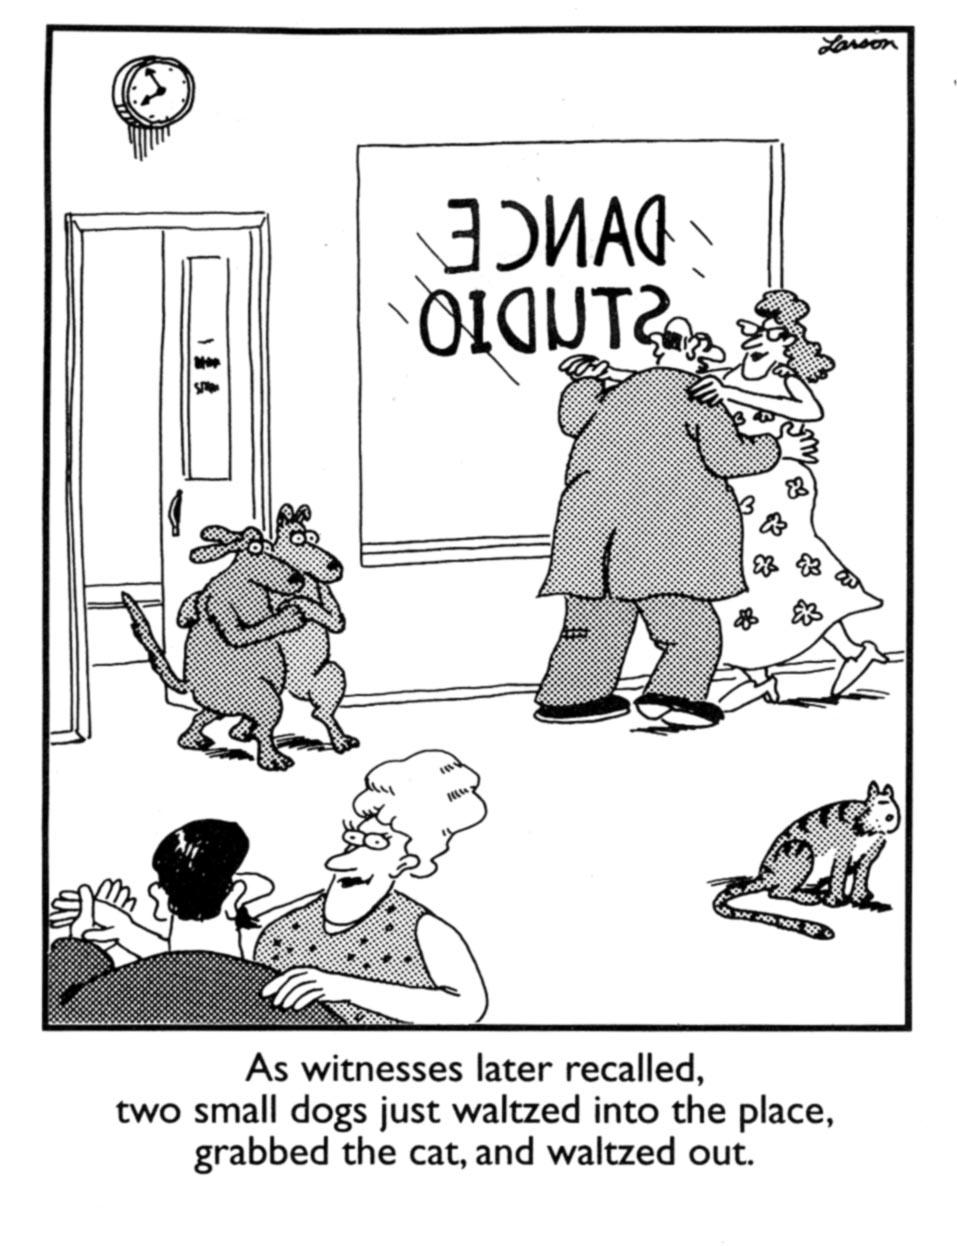
\includegraphics[width=0.75\textwidth]{graphics/example_cartoon.png}
	\captionsetup{labelformat=empty}
	\caption{Cartoon by Gary Larson}
	\label{fig:fig1}
\end{figure}
\end{dedication}
\clearpage

\chapter{Introduction}

\section{Aim} \label{aim}
This diploma thesis aims to research whether computers are capable of understanding humor by learning Gary Larson's cartoons. This was done by training several deep neural networks. Their task was to predict the funniness of a cartoon better than simple baselines. Even though humor is intrinsicly subjective, the available data allowed quantitative comparisons using the chosen metrics (accuracy and mean absolute error). The goal was to find the best neural network architecture for predicting the funniness of a cartoon.

Furthermore, based on Gary Larson's cartoons a new data set for computational humor was created, which could help further research in this area.

The questions this work tries to answer, are the following:

\begin{enumerate}

\item Which neural network architecture is best suited for predicting the associated funniness of each cartoon?

\item Do the trained models outperform previously defined baselines? These baselines include most frequent funniness, average funniness, uniform random funniness and stratified random funniness.

\item If a model outperforms the baselines, does it generalize and understand humor? The model could instead exploit spurious statistical cues in the dataset similar to Niven et al. \cite{cleverhans}

\item Which feature domain is best suited for predicting the funniness: Is using both visual and text input better than they perform individually?

\end{enumerate}

On a higher level this thesis tries to bring subjectivity considerations into computational humor. Previous work in this field did not model the humor of a single person, but instead focused on what humans collectively consider humorous. The novel dataset and deep learning enable this new perspective.

\section{Motivation}

Based on the recent success of deep learning in fields such as self-driving cars \cite{selfdriving}, speech recognition \cite{speech}, machine translation \cite{nmt}, etc., one could expect similar success in computational humor. Especially natural language processing and image-related tasks have seen significant improvements of the state-of-the-art through deep neural architectures.

Initially the idea of this thesis was, that the trained model might have been able to extract certain patterns of humor. Gary Larson's cartoons can be grouped into several themes. For example stone age, scientist or cats versus dog are common themes he uses. A competent model could distinguish these themes and might find patterns of humor among these subjects. Someone might find stone age themed cartoons funnier than cats versus dogs cartoons. 

Important to note is that preference is very subjective. The model must be trained by data of the same person, because otherwise the personal preference might be lost. If trained successfully it would open a whole set of new research possibilities: The study of humor of people through the lense of deep neural networks. This is especially interesting, since it has been shown that there are key similarities between how deep neural networks work and how the human brain works. \cite{Cichy2016}

For example if such a model were possible, it could possibly allow a more formal comparison of humor between different authors or different people.
The same model might be able to be transferred to the work of other authors. Depending on how well this transfer works, one could argue whether the humor of these authors are similar or not, given the annotator's sense of humor. Also the trained model themselves could contain interesting features. Possibly a functioning model could develop a cat-detecting neuron, which could reveal insights into human humor.

Another key motivation was in the creation of the underlying data set: This thesis uses a novel data set, where each cartoon was paired with a funniness annotation of the same person. This allows to quantitatively evaluate the humor of a single person, as the data set is comparatively large. The scope of the data set is also unique, as there is no other data set with similar cartoons available. In future the same data set could be used for other tasks. A very hard, but very interesting task would be using a generative architecture, such as generative adversarial network (GAN) to generate a funny cartoon image from a punchline. Or vice versa: Generating a funny punchline from a cartoon image. And finally generating completely new funny cartoons with fitting punchlines.\cite{gan2}\cite{gan}

In recent years more and more deep learning techniques have been applied in the field of computational humor. One problem of these approaches is that they do not take the subjectivity of this problem into account. Humor differs from person to person and also changes over time significantly. For example in Chiruzzo et al \cite{chiruzzo2019overview} the corpus was extracted from twitter where each tweet was classified as humorous or not humorous. The ground truth classification was annotated using crowd sourcing. The problem with such data sets is that the funniness is determined by some form of average. Some individuals might find the same text very humorous, while other individuals might find it not humorous at all. The crowd sourcing hides this fact by averaging. Therefore, these data sets and models usually do not learn the humor of a single person, but instead what most people generally find funny (or not funny). This is very important and also reveals interesting insights into humor, but this thesis' motivation is to focus more on the subjectivity of this topic.

This work finally shows that humor is still a hard problem and current deep learning architectures are not yet capable of generalizing humor in the chosen context of this thesis. Further research is still needed, especially since, if successful, it would enable many new research possibilities.


\section{Methodology}

Firstly I performed a detailed literature survey. The goal was to get a grasp of the state-of-the-art of deep learning in the field of computational humor, image classification, natural language processing and humor in general.

Next I did the data acquisition, in which the ground truth was created: A data set of Gary Larson's cartoons with funniness annotations was created. These cartoons were prepared such that they could be used for training the neural networks effectively. This included cropping, resizing and filtering the cartoons. Extracting the punchlines, as well as annotating the funniness.

I performed the following steps iteratively. This allowed to adapt to the challenges which occured during the course of this research:

\begin{enumerate}

\item I picked an architecture candidate and designed it accordingly. This was based on prior knowledge and previous literature research.
\item Then I implemented and trained the architecture.
\item Afterwards I evaluated the resulting model. Problems were determined and possible solutions analyzed.

\end{enumerate}

At first the focus was on visual-only models. Then the focus shifted towards text-only models. Finally I evaluated several approaches that combine both text- and visual features into a single model. Also the architectures went from simple to more complex per iteration.

Finally I performed a detailed evaluation. The most interesting models were picked and analyzed thoroughly. Goal of this phase was to find answers to the questions listed in section \ref{aim}.
%\pagebreak
\section{Overview over thesis}
This section gives a short overview over the contents of this thesis.

Chapter 2 (Background) contains the background necessary for this thesis. Topics covered are computational humor, machine learning, artificial intelligence, neural networks, natural language processing, automated machine learning and an overview over related work.

Chapter 3 (Design) covers the iterative design process of this thesis. This process began with the visual component of Gary Larson's cartoons using convolutional neural networks. Next, design shifted towards the development of deep neural networks for punchlines using LSTMs, AutoML, feed-forward neural networks and word embeddings. And finally this chapter outlines the combination of both domains in a single architecture.

Chapter 4 (Implementation) focuses on the implementation aspects of the previously described neural network architectures. The reader gets an overview over the technology chosen and I implemented the the architectures.

Chapter 5 (Evaluation) gives the reader an insight into the final results obtained by selected interesting architectures, compared to the baselines. I examine the inner working of the models, outlining their mistakes using confusion matrices and other techniques.

Chapter 6 (Conclusion) finalizes this thesis with lessons learned during the course of the development of this work. 


\chapter{Background}

As this work combines the field of computational humor with deep learning, an understanding of both fields is required. This chapter contains the required background for this thesis. First an overview of artificial intelligence and and machine learning is outlined. Section \ref{nlpbackground} lays out techniques of natural language processing. Section \ref{transferlearning} gives an overview over a technique called transfer learning. The next section (\ref{automlbackground}) outlines automated machine learning. Based on the previous sections I summarize the research area of computational humor in section \ref{comphumorbackground}. This chapter ends with related work of traditional computational humor and deep learning based computational humor in section \ref{relatedworkbackground}.

\section{Machine Learning and Artificial Intelligence}
The field of Artificial Intelligence (AI) tries to reproduce (human) intelligence using computers \cite{questforai}. It is yet impossible to develop a truly intelligent computer program, also known as strong AI \cite{strongweakai}. AI researchers typically pick certain narrow subtasks of what is considered to require intelligence. Such a system is also known as weak AI \cite{strongweakai}. These tasks usually entail some utility for other application domains and range from image classification, self driving cars to machine translation.

\subsection{History of Artificial Intelligence}

In the year 1950 Alan Turing proposed the idea of a test which could determine if machines have human-level intelligence. In this test a human chats with a human and a computer. Both try to convince the human that they are a real human being. If the human is not reliably able to tell them apart, then the computer passes the Turing test \cite{turingtest}.

In the 1960s and 70s AI researchers overestimated the possibilities of their systems greatly. For example, Marvin Minsky (a key researcher back then) said in 1970: "In from three to eight years we will have a machine with the general intelligence of an average human being." The goal of artificial intelligence initially seemed tractable:
The computational power of computers increased exponentially and new algorithms and methods were developed \cite{mooreslaw}\cite{questforai}. The first chatbot (ELIZA) by Joseph Weizenbaum which showed how communication between humans and machines could be implemented using relatively simple rules seemed promising \cite{weizenbaum1966eliza}.

There were many schools of thoughts, among these were: The symbolic-based approach and the connectionism-based approach \cite{machineswhothink}. Symbolic-based systems reached early success, by applying logic reasoning to AI \cite{machineswhothink}. The idea of connectionism was to model AI systems using the human brain as a blueprint \cite{machineswhothink}. In the end of the 60s many AI researchers lost interest in connectionism, as the limitations of the perceptron were revealed \cite{Minsky1969PerceptronsA}. This insight halted the research in this area for many years \begin{flushleft}
\cite{questforai}
\end{flushleft}.

The symbolic-based approach initially showed much success in several tasks (for example: theorem proving \cite{aimodern}) but also reached a limit. The general approach was to model reasoning as a form of search \cite{aimodern}
: Proceed step-by-step towards the goal and backtrack if the steps lead to a dead end. The problem with this approach is the sheer size of the search space. The combinatorial explosion is intractable and can only be handled by heuristics, which limit the power of the system \cite{aimodern}. The limiting capabilities of perceptrons and the lack of progress in key areas resulted in the first AI winter \cite{crevier}. Funding was cut to a minimum \cite{crevier}.

Expert systems dominated the 1980s \cite{machineswhothink}. These were systems which were crafted by human experts and entailed their knowledge of the specific domain it tried to model using logical rules \cite{questforai}. One important contribution of expert system was their usefulness. Even early experiments managed to diagnose infectious blood diseases \cite{questforai}. 

Research in the field of connectionism continued as well. Backpropagation solved issues of previous attempts \cite{questforai}\cite{aimodern}. Training larger neural networks was now tractable. One of the most popular architectures of the time is the Hopfield network which models an associative memory \cite{anintroductiontoneuralnetworks}. Still, the expectations were not met and the second AI winter emerged during the late 1980s \cite{machineswhothink}. This time it not only hit the scientific community, but also many AI companies \cite{questforai}.

During the 1990s AI had a slightly negative connotation \cite{avoidai}: AI-based systems were working in the background and many problems were largely solved (for example speech recognition and information retrieval \cite{avoidai}\cite{historyinformationretrieval}). A big milestone of AI research was achieved, when Deep Blue managed to win against the best chess player of the time, Garry Kasparov \cite{questforai}. This was largely due to the increased computational power and clever engineering, instead of some new paradigm \cite{questforai}.

During this period the collaboration with other research fields began\cite{aimodern}. For example, knowledge from mathematics and economics were applied in AI. Especially decision theory and probability theory brought in very important techniques, such as hidden Markov models and Bayesian networks \cite{statisticsinml}\cite{aimodern}.

The next boom in the field of AI was fueled by Deep Learning and the success it had in many problems of artificial intelligence \cite{selfdriving}\cite{nmt}\cite{speech}. Beginning with the convolutional neural network AlexNet which was the first approach that reached a top-5 error of 15.3\% on the ImageNet Large Scale Visual Recognition Challenge in 2012. \cite{alexnet}

And then continuing in 2016 with AlphaGo winning against one of the best human player of the board game Go \cite{alphagopaper}. Compared to chess Go is a much more difficult game to play for computers, as the combinatorial explosion is much larger and the heuristics available are much weaker in Go compared to chess \cite{alphagopaper}.

The next frontier of artificial intelligence is not clearly established yet, as the progress of deep learning is very fast. For example the team behind AlphaGo applied similar techniques to real time strategy games successfully \cite{arulkumaran2019alphastar}. It seems that especially tasks requiring long time planning or deep understanding of the underlying structure is a problem \cite{atariplaying}. For example this work shows that understanding humor is still very challenging.

%The danger of a third AI winter is greater than never. Despite the recent advances, researchers must be wary to not overestimate the power of AI. The question remains, whether current technology allows for strong AI, or if there is some limit we cannot advance using current approaches.

\subsection{Machine Learning}

Machine Learning (ML) is a domain of AI \cite{aimodern}. Machine learning tries to build a model which generalizes as good as possible to previously unseen data by learning automatically from a training data set \cite{bishop}. Learning means extracting patterns from the data set by applying a machine learning algorithm \cite{bishop}. Models can be parametric or non-parametric. A parametric model means that the general function is fixed and can only be adjusted by adapting the parameters \cite{aimodern}. For example neural networks are parametric, as gradient descent adjusts the weights and biases for each neuron during training, while the general structure of the neural network is not. In contrast, for a non-parametric model the machine learning algorithm learns the function itself \cite{aimodern}. An example for this type of model would be k-Nearest Neighbor.  Since the focus of this work are neural networks we will discuss parametric models in more detail.

More formally, a model is a function $\boldsymbol{y}(\boldsymbol{X}, \boldsymbol{\theta})$ where $\boldsymbol{X}$ is the training data and $\boldsymbol{\theta}$ are the parameters of the model \cite{bishop}. Through some optimization algorithm (for example gradient descent) the model is adjusted such that it generalizes ("learns") the underlying structure \cite{anintroductiontoneuralnetworks}. This model should make good predictions for previously unseen samples. Important is the distinction between model parameters ($\boldsymbol{\theta}$) and model hyperparameters \cite{aimodern}. Model hyperparameters are parameters which cannot be estimated from the available data and are typically set by a human arbitrarily heuristically \cite{hyperparameter}. A parameter on the other hand, can be estimated from the data, given the previously set hyperparameters \cite{anintroductiontoneuralnetworks}.

The data $\boldsymbol{X}$ is a matrix where each row is a sample and each column a feature. A feature is an individual measurable property or characteristic of a phenomenon being observed \cite{bishop}. For example when trying to apply a machine learning task on an image one could use the red, green and blue channel values of each pixel as a feature. Choosing appropriate features is a difficult task and can make or break the performance of the trained model.

Machine learning tries to approximate a function from the selected data set. Depending on the available information, different strategies must be applied. Typically, the most convenient and preferred mode is supervised machine learning \cite{aimodern}. Supervised means that not only the data $\boldsymbol{X}$ is available, but also the target values $\boldsymbol{t}$. This means that the problem can be relatively easily solved using an optimization algorithm. More formally we try to find a $\boldsymbol{\theta}$ such that $\boldsymbol{y}(\boldsymbol{X}, \boldsymbol{\theta}) = \boldsymbol{t}$. If the $\boldsymbol{t}$ labels are not available, then unsupervised machine learning is typically applied \cite{aimodern}. For example clustering methods allow unsupervised ML. If a mixture of labelled and unlabelled data is available, machine learning practitioners apply semi-supervised machine learning \cite{semisupervised}.

Additionally, there is a distinction between classification and regression tasks \cite{bishop}. If $\boldsymbol{t}$ is a continuous variable, machine learning practitioners call it a regression task and the model is a regressor. Otherwise, if $\boldsymbol{t}$ is categorical and can only take finite  values, then machine learning practitioners call it a classification task and the model is a classifier. An example for a regression task is stockmarket prediction, where the model predicts the stock price of some stock. An example for a classification task is spam detection. Such a model predicts whether an e-mail is spam or not (binary classification). Often a regression task can be modelled as a classification task by converting the features using discretization and vice versa \cite{discretization}. Instead of predicting the stock market directly, one can instead predict classes and use the average value of each bucket as the predicted stock price. Refer to table \ref{table:conversionregressclass} for an example. The right approach is highly task dependent \cite{aimodern}.

\begin{table}[]
\centering
\begin{tabular}{|l||l|l|l|l|}
\hline
Regression Value & $<50$ & $51 - 100$ & $101 - 200$ & $200<$ \\
\hline
Classification Class & CLASS 50      & CLASS 75 & CLASS 150 & CLASS 250 \\
\hline
\end{tabular}
\caption{Example for the conversion between regression and classification tasks }
\label{table:conversionregressclass}
\end{table}

\subsection{Training of Machine Learning models} \label{trainingofml}

The most important property of a model $\boldsymbol{y}$ is the generalization power for unseen data \cite{bishop}. Training a model $\boldsymbol{y}$ which predicts the training data $\boldsymbol{X}$ perfectly is trivial: The machine learning algorithm could always build a lookup table which memorizes a mapping from the training samples to the target labels $\boldsymbol{t}$ \cite{overfitting}. If this happens, it is called \textit{overfitting} \cite{overfitting}.

The \textit{holdout method} facilitates the approximation of the performance of a model $\boldsymbol{y}$ for previously unseen data \cite{holdoutcrossvalidation}. There is often some bias towards the original data set \cite{datasetbias}. The better the data set characterizes the underlying problem, the better the final model may perform practically \cite{datasetshift}. For example, if one trains a vehicle detection model, but the data set does not include any images of motorcycles, then the model will perform badly in the real world. Regardless of the method applied, the model would not be able to detect motorcycles - despite the performance metrics possibly indicating otherwise.

The holdout method first splits the data into three distinct subsets: Training, validation and test set \cite{holdoutcrossvalidation}. Then the practitioner incrementally adjusts the hyperparameters and trains on the training set, based on the performance of the model on the validation set \cite{holdoutcrossvalidation}. Finally, to gather the true performance the practitioner has to evaluate on the test set \cite{holdoutcrossvalidation}. The following algorithm illustrates the holdout method using pseudo code:

\begin{algorithm}
\caption{Holdout method \cite{holdoutcrossvalidation}}\label{holdoutalgo}
Take the data set $\boldsymbol{X}$ and split randomly into three distinct sub sets: Training, validation and test set.

\While {$\neg$some halting criterion} {
Train the model on the train split.

Check performance of the trained model on the validation set.

Manually adjust hyperparameters such that the model generalizes better
}

Check final performance on the test set of the best trained model

\end{algorithm}

This variant is also commonly referred to as the three-way holdout method \cite{holdoutcrossvalidation}. The validation/test split is only needed if there are hyperparameters which are being optimized iteratively \cite{holdoutcrossvalidation}.
Due to the lack of standardization, sometimes the validation set is actually called the test set and the test set the validation set \cite{patternrecognitionandnn} \cite{anintroductiontoneuralnetworks}.

Commonly used halting criteria include:
\begin{itemize}
\item Maximum number of iterations \cite{kerashalting}
\item Plateauing performance: No improvement after a previously defined number of iterations \cite{haltingcriteria}
\item Maximum performance: The model reaches a certain performance threshold \cite{kerashalting}
\item Combination of multiple halting criteria \cite{kerashalting}
\end{itemize}

\if false
A common split ratio for the training/validation and test set is \cite{holdoutcrossvalidation}:
\begin{enumerate}
\item 60\%: Training Set
\item 20\%: Validation Set
\item 20\%: Test Set
\end{enumerate}
\fi

If there is no clear separation between the test and training set, a machine learning practitioner calls it a data leakage \cite{doingdatascience}. The actual performance of the trained model $\boldsymbol{y}$ could be potentially much worse for unseen data than the metrics suggest. Selecting the best performing model, instead of the last model is called early stopping or the pocket algorithm.

Another method for evaluating the performance of a machine learning model is called \textit{cross-validation} \cite{holdoutcrossvalidation}: This method randomly splits the data into $n$ partitions. Then $n$ models are trained for each partition, where the partition is the test set and the remaining data is the training set. In general cross validation approximates the performance better than the holdout method \cite{aimodern}. As many models are trained (depending on $n$) it can be computationally very expensive  \cite{bishop}.

The following pseudo code illustrates cross-validation, which first splits the data in a $\boldsymbol{TRAIN}$ and a $\boldsymbol{TEST}$ set \cite{holdoutcrossvalidation}. Then incrementally the $\boldsymbol{TRAIN}$ set is split into $k$ partitions $\boldsymbol{P}$. For each $(\boldsymbol{TRAIN} \setminus \boldsymbol{P}, \boldsymbol{P})$ pair a model is trained and evaluated \cite{bishop}. Based on the overall performance the practitioner adjusts the hyperparameters accordingly. Finally the $\boldsymbol{TEST}$ set evaluation returns the performance on unseen data \cite{holdoutcrossvalidation}.

\begin{algorithm}
\caption{Cross-validation method \cite{holdoutcrossvalidation}}\label{holdoutalgo}
Take the data set $\boldsymbol{X}$ and split randomly into two distinct sub sets: Training ($\boldsymbol{TRAIN}$) and test set ($\boldsymbol{TEST}$).

\While {$\neg$some halting criterion} {
Take the train set $\boldsymbol{TRAIN}$ and split into $k$ partitions

\ForEach{partition $\boldsymbol{P}$}{
Train the model on $\boldsymbol{TRAIN} \setminus \boldsymbol{P}$

Calculate performance on $\boldsymbol{P}$
}

Calculate average performance

Manually adjust hyperparameters such that the model generalizes better.
}

Check final performance on the test set $\boldsymbol{TEST}$ of the best trained model

\end{algorithm}

Depending on the machine learning task and applied methodology, there is no distinct test set \cite{holdoutcrossvalidation}. Figure \ref{fig:holdoutvscv} compares the splits of holdout method and cross validation.

\begin{figure}[ht]
	\centering
  	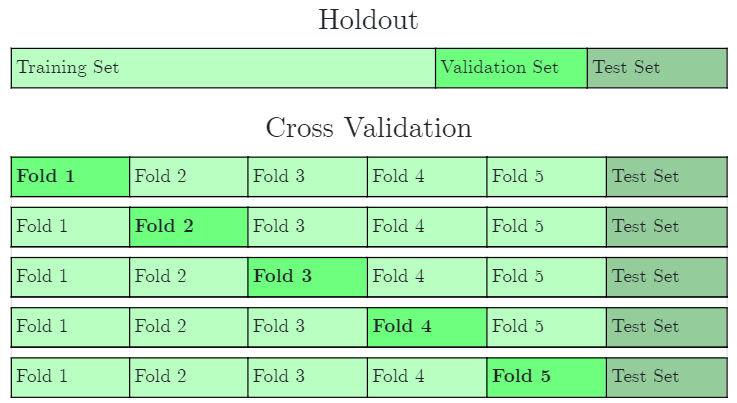
\includegraphics[width=0.75\textwidth]{graphics/holdoutvscv.png}
	\caption{Comparison of the splits between holdout and 5-fold cross validation}
	\label{fig:holdoutvscv}
\end{figure}

\subsection{Evaluation of Machine Learning models}

Measuring the performance of a model $\boldsymbol{y}$ is an important aspect of proper machine learning \cite{performanceevaluation}. Choosing the performance measure is highly task dependent \cite{performanceevaluation}. For this thesis the mean absolute error (MAE) and the accuracy were determined to be suited \cite{accuracy}. Other metrics considered were F1 and mean squared error (MSE) \cite{accuracy} \cite{Powers2008EvaluationFP}.

\subsubsection{Mean absolute error and mean squared error}
\begin{equation}
\text{MAE} = \frac{1}{n}\textstyle \sum_{i=1}^n \displaystyle\mid \hat{X}_i - X_i \mid
\end{equation}
\begin{equation}
\text{MSE} = \frac{1}{n}\textstyle \sum_{i=1}^n \displaystyle\left( \hat{X}_i - X_i \right)^2
\end{equation}
\begin{align*}
\text{where}~\hat{X}&~\text{is the predicted sample} \\
X&~\text{is the ground truth}
\end{align*}

MAE is interesting because a near miss is less penalized \cite{accuracy}. For example, if a model predicts funniness of 5, while the real funniness is 6, the term $\mid 5 - 6 \mid = 1$. On the other hand if the predicted funniness were a 2, the term $\mid 2 - 6 \mid = 4$. The lower the MAE the better.

MSE works similarly to MAE, but errors are penalized more \cite{accuracy}. The calculations for the above examples are $\left( 5 - 6 \right)^2 = 1$ and $\left( 2 - 6 \right)^2 = 16$, which is a significant difference. For a very noisy dataset MAE is usually better suited than MSE.

\subsubsection{Accuracy and F1}

\begin{equation}
\text{Accuracy}=\frac{|\text{True Positives}| + |\text{True Negatives}|} {|\text{True Positives}| + |\text{True Negatives}| + |\text{False Positives}| + |\text{False Negatives}|}\\
\end{equation}
\begin{align*}
\text{where}~|\text{True Positives}|&~\text{is the number of correctly classified samples of the positive class} \\
|\text{True Negatives}|&~\text{is the number of correctly classified samples of the negative class} \\
|\text{False Negatives}|&~\text{is the number of incorrectly classified samples of the negative class} \\
|\text{False Positives}|&~\text{is the number of incorrectly classified samples of the positive class} \\
\end{align*}

Accuracy is easy to understand and is commonly applied in classification tasks \cite{accuracy}. The higher the accuracy the better \cite{Powers2008EvaluationFP}. But the accuracy metric might hide important weaknesses of a model \cite{accuracy}:

Consider the following example: The task is evaluating a model which predicts whether a patient has cancer or not. The test dataset is highly imbalanced, and contains 99 samples of patients without cancer and 1 sample of a patient with cancer. If the model always predicts that a patient has no cancer, the resulting accuracy is 99\%. 

F1 scores handles such cases better, by emphasizing false negatives and false positives more \cite{Powers2008EvaluationFP}. It is the harmonic mean of the precision and recall score \cite{Powers2008EvaluationFP}:

\begin{equation}
\text{Precision}=\frac{|\text{True Positives}|} {|\text{True Positives}| + |\text{False Positives}|}\\
\end{equation}
\begin{equation}
\text{Recall}=\frac{|\text{True Positives}|} {|\text{True Positives}| + |\text{False Negatives}|}\\
\end{equation}
\begin{equation}
\text{F1} = 2 * \frac{\text{Precision} * \text{Recall}}{\text{Precision} + \text{Recall}}
\end{equation}

For multi class classification (more than two possible classes) a confusion matrix helps to visualize the predictions of a model \cite{accuracy}. The rows of a confusion matrix are usually predicted classes and the columns the ground truth. A perfect model would show 100\% along the diagonal of the matrix, as there would be no wrong classifications.

A confusion matrix usually reveals common mistakes of a model \cite{accuracy}. For example if a model never predicts a class, it can be easily detected using this visualization. For an example of a confusion matrix please refer to figure \ref{fig:confusionmatrixtransferlearningtest}.

\section{Neural Networks}

Before neural networks, there was the perceptron \cite{questforai}. It is a binary classifier and uses a linear function to perform classification \cite{Minsky1969PerceptronsA}. Binary refers to the fact, that a simple perceptron can only distinguish between two states. The learning process starts with a random decision boundary, which is iteratively adapted such that the number of misclassifications is minimized \cite{aimodern}. Due to the linear decision boundary the perceptron is only able to learn decision boundaries that are linearly separable \cite{questforai}. For example, a simple XOR (table \ref{xor}) cannot be learned by a basic perceptron. This motivated the introduction of multi layer perceptrons (MLPs), since they are in theory able to approximate any function, given a nonlinear activation function \cite{universalfunction}. An MLP consists of multiple perceptrons grouped in layers and each layer connects with the previous layer \cite{bishop}. MLPs are feed forward neural network \cite{bishop}.

\begin{table}[]
\centering
\begin{tabular}{|l|l|l|}
\hline
XOR & 0 & 1 \\ \hline
0   & 0 & 1 \\ \hline
1   & 1 & 0 \\ \hline
\end{tabular}
\caption{XOR function}
\label{xor}zs
\end{table}


\begin{figure}[ht]
	\centering
  	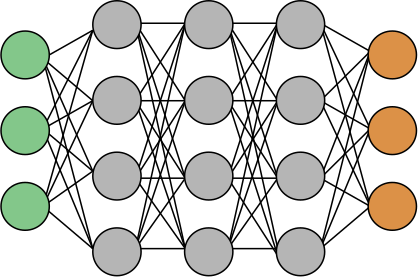
\includegraphics[width=0.75\textwidth]{graphics/simple_neural_network.png}
	\caption{Fully Connected Feed Forward Neural Network}
	\label{fig:feedforward}
\end{figure}

Part of the reason why neural networks are so powerful, especially deep neural networks, stems from their flexibility \cite{selfdriving}\cite{speech}\cite{nmt}. They can adapt to many different domains very easily. Illustrated at Figure \ref{fig:feedforward} is a fully connected feedforward neural network with 3 hidden layers. Neural networks can have many more layers (refer to section \ref{dlbackground}) or even contain loops (section \ref{lstmbackground}).

A neural network generally consists of multiple neurons, layers and connections \cite{aimodern}. The general inspiration for them is the human brain which also consists of similar building blocks \cite{anintroductiontoneuralnetworks}.

In the human brain neurons receive their signals through dendrites (connections in neural networks) and are then sent through the axon to other neurons \cite{anintroductiontoneuralnetworks}. The signal strength is adjusted (analogous to activation functions in neural networks) such that other neurons in the brain are more stimulated \cite{anintroductiontoneuralnetworks}. Note that key parts of the human brain are not simulated in a neural network: During training the weights and biases are adjusted using gradient descent, for more information refer to section \ref{nntrain} \cite{recentexcitementabotuneuralnetworks}. Nevertheless neural networks (especially convolutional neural networks) produce similar structures also observed in the human brain \cite{Cichy2016}.


\if false
Seiten: 1.5

\begin{itemize}

\item Am Anfang war das Perceptron: Ursprüngliche Idee und Limitation (XOR). Trainingsprozedur kurz anschneiden.
\item Dann auf MLPs weiter: Erlaubt lernen von arbiträren Funktionen (zB XOR).
\item Zu Neuronale Netzwerke: Differenzierbar => effizienteres Trainieren
\item Illustration eines simplen 3 Layer Neuronalen Netzwerks
\item "Inspiration" von neuronalen Netzwerken ziehen: Menschliches Gehirn

\end{itemize}

\fi

\subsection{Basics of neural networks}

From a different perspective, neural networks can also be seen as a series of functional transformations of some input vector into an output vector \cite{colahbackprop}. Given the input $x_1, ..., x_D$ and $M$ connections the input layer can be described as \cite{bishop}:
\begin{equation}
a_j = \sum_{i=1}^{D} w_{ji}^{(1)}x_i + w_{j0}^{(1)}
\end{equation}

where $j = 1, ..., M$. $w_{ji}^{(n)}$ is usually referred to as weights and $w_{j0}^{(n)}$ as biases. $a_j$ is called an activation, which is then transformed using a nonlinear, differentiable activation function $h(\cdot)$ \cite{bishop}:
\begin{equation}
z_j = h(a_j)
\end{equation}
Depending on the problem different activation functions are applied. Common functions include:
\begin{itemize}
\item Tanh function \cite{activationfunctions}: zero-centered function between -1 and 1 \cite{activationfunctions}. Suffers from the vanishing gradient problem \cite{activationfunctions}.
\begin{equation}
h(x) = \dfrac{e^x - e^{-x}}{e^x + e^{-x}}
\end{equation}
\item Sigmoid Function \cite{anintroductiontoneuralnetworks}: "Squashes" the input value between 0 and 1 \cite{anintroductiontoneuralnetworks}.
\begin{equation}
h(x) = \dfrac {1} {1 + e^{-x}}
\end{equation}
\item ReLU (Rectified Linear Unit) \cite{Goodfellow-et-al-2016}: Very commonly used in deep learning, as it performs very well on a wide range of different tasks \cite{activationfunctions}. Can be calculated very quickly, as it does not contain any division or exponential \cite{activationfunctions}.
\begin{equation}
h(x) = max(0, x)
\end{equation}
\item SoftMax \cite{Goodfellow-et-al-2016}: Used to transform any vector into a probability distribution \cite{activationfunctions}. This is commonly used for the final layer of classification tasks with multiple classes (multi class classification) \cite{activationfunctions}.
\begin{equation}
h(\boldsymbol{x}) = \dfrac{e^{x_i}}{\sum_{k=1}^{M} e^{x_k}}
\end{equation}
\item Logistic Sigmoid \cite{Goodfellow-et-al-2016}: Similar to SoftMax, but used for binary classification \cite{Goodfellow-et-al-2016}.
\begin{equation}
\sigma(x) = \dfrac{1}{1 + exp(-x)}
\end{equation}
\end{itemize}


For the first hidden layer of a neural network the following values are linearly combined \cite{bishop}:
\begin{equation}
a_k = \sum_{i=1}^{M} w_{kj}^{(2)}z_j + w_{k0}^{(2)}
\end{equation}

where $k = 1, ..., K$ is the total number of outputs of the first hidden layer. The same procedure is repeated for the remaining hidden layers \cite{bishop}. The final result for classification tasks is usually obtained by applying a softmax activation function of the last layer's output \cite{bishop}.

Combining these transformations together for a relatively simple two layer network results in the following equation:

\begin{equation}
y_k(\boldsymbol{x}, \boldsymbol{w}) = \sigma\left(\sum_{i=1}^{M} w_{kj}^{(2)}h\left(\sum_{i=1}^{D} w_{ji}^{(1)}x_i + w_{j0}^{(1)}\right) + w_{k0}^{(2)}\right)
\end{equation}

This term can be simplified, by assuming that the input vector $x$ has always a constant term with the value $1$ \cite{bishop}. As this removes the additional addition for the bias for each layer.

\begin{equation} \label{forwardcalculation}
y_k(\boldsymbol{x}, \boldsymbol{w}) = \sigma\left(\sum_{i=1}^{M} w_{kj}^{(2)}h\left(\sum_{i=1}^{D} w_{ji}^{(1)}x_i\right)\right)
\end{equation}

Evaluating \ref{forwardcalculation} is called forward propagation \cite{colahbackprop}.

\if false
Seiten: 1.5
\begin{itemize}
\item Neuronale Netzwerke formal definieren: Konkatination von differenzierbaren funktionen
\item Activationfunction angeben und kurz den Verwendungszweck erwähnen: tanh, sigmoid, Softmax, ReLU, Logistic Sigmoid
\item Mathematische Definition eines Layers
\item Kombinieren mehrere Layers mathematisch
\item Simplifizierung, indem Bias als konstanten Input mit 1 "versteckt" wird

\end{itemize}

\fi

\subsection{Training of neural networks} \label{nntrain}

For training a loss function $L(\boldsymbol{w})$ is defined, where $\boldsymbol{w}$ are the trained weights \cite{Goodfellow-et-al-2016}.

The loss can have many different forms, but in the following we will discuss primarily the cross entropy loss, since it is commonly used for classification tasks \cite{dlvc}.

\begin{equation}
L(\boldsymbol{w}) = -\sum_{n=1}^N \left( t_n\,\text{ln}\, y_n + (1 - t_n)\,\text{ln}(1 - y_n)\right) \text{ where } 
y_n = y(\boldsymbol{x_n}, \boldsymbol{w})
\end{equation}

Generalized for multiclass classification with $K$ mutually exclusive one hot encoded classes \cite{dlvc}:

\begin{equation}
L(\boldsymbol{w}) = -\sum_{n=1}^N \left(\,\sum_{k=1}^K \left(t_{kn}\,\text{ln}\,y_k(\boldsymbol{x_n},\boldsymbol{w})\right)\right) \text{ where } y_k(\boldsymbol{x}, \boldsymbol{w}) = \text{SoftMax}(\boldsymbol{y}(\boldsymbol{x_k}, \boldsymbol{w}))
\end{equation}

For regression tasks the L1 loss can be used \cite{accuracy}:

\begin{equation}
L(\boldsymbol{w}) = \dfrac{1}{N} \sum_{n=1}^N |x_n - y_n| \text{ where } 
y_n = y(\boldsymbol{x_n}, \boldsymbol{w})
\end{equation}

The goal of training neural network is to minimize the loss of the model \cite{dlvc}:

\begin{equation}
\text{arg min}\quad L(\boldsymbol{w})
\end{equation}

Training takes advantage of the fact that it is a function composition of differentiable functions \cite{Goodfellow-et-al-2016}. This allows the use of a technique called gradient descent \cite{anintroductiontoneuralnetworks}. The idea is intuitive: Walk along the path with the steepest descent until some halting criterion is met \cite{anintroductiontoneuralnetworks}. Because the neural network is differentiable the steepest descent is relatively easily obtained, by taking the negative of the first derivative of the loss function \cite{Goodfellow-et-al-2016}. A halting criterion could be one described in section \ref{trainingofml}. Algorithm \ref{gradientedescentalgo} illustrates the pseudo code of gradient descent.

\begin{algorithm}
\caption{Gradient descent pseudo code \cite{anintroductiontoneuralnetworks}}\label{gradientedescentalgo}
\While {$\neg$some halting criterion} {
Compute gradient: $\boldsymbol{w}' = \bigtriangledown	L(\boldsymbol{w})$

Update weights: $\boldsymbol{w} := \boldsymbol{w} - \alpha \boldsymbol{w}'$
}

\end{algorithm}

$\alpha > 0$ is a hyperparameter and called the learning rate \cite{Goodfellow-et-al-2016}. $\alpha$ is usually set empirically \cite{Goodfellow-et-al-2016}. A too high learning rate (for example $\alpha = 1$) means that the loss of the neural network could oscillate  violently, where the loss function often increases significantly \cite{Goodfellow-et-al-2016}. The lower $\alpha$ the more likely it is that the gradient descent converges in a local optima \cite{Goodfellow-et-al-2016}. Figure \ref{fig:gradientdescent} illustrates the process of gradient descent. % Usually in the beginning of training the learning rate should be higher and at the end the learning rate should be lower. This is the reason why it is common to apply learning rate decay during training. This means that the learning rate is gradually reduced during the learning

\begin{figure}[ht]
	\centering
  	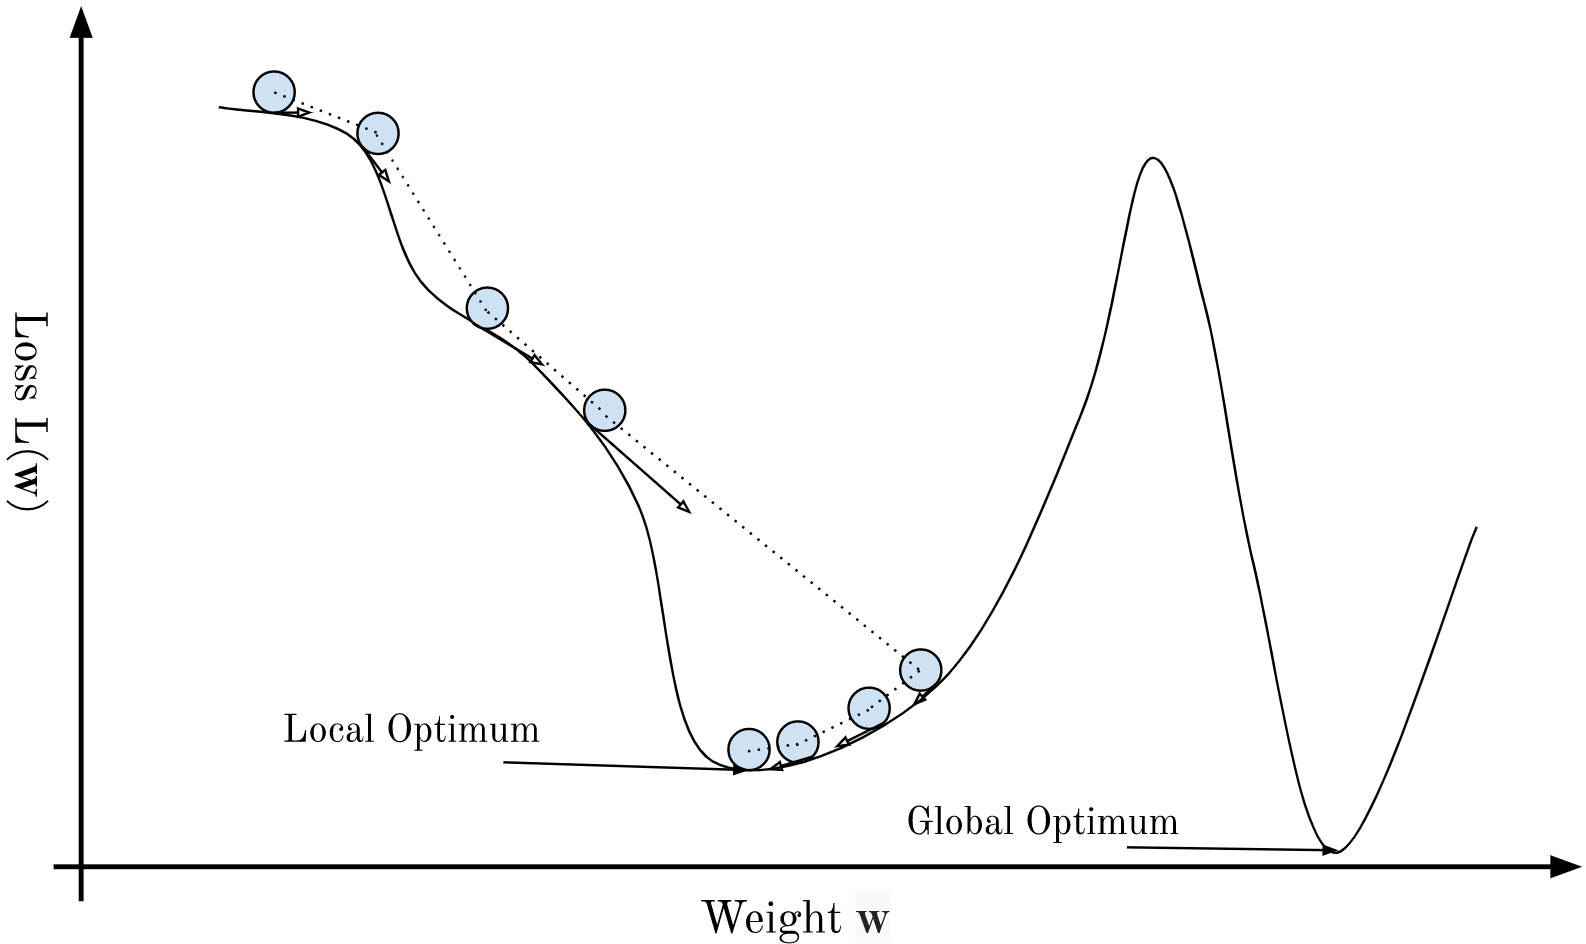
\includegraphics[width=0.85\textwidth]{graphics/gradientdescent.png}
	\caption{Visual representation of gradient descent with momentum. Longer arrows mean steeper gradient. \cite{Goodfellow-et-al-2016}}
	\label{fig:gradientdescent}
\end{figure}

\if false
Seiten: 1.5
\begin{itemize}
\item Loss erklären (Für Training benötigt)
\item Für Klassifizierung: Cross Entropy Loss
\item Für Regression: L1 Loss
\item Gradient Descent erklären
\item Simpler Pseudocode für Gradient Descent
\item Halting Kriterium
\item Illustration von Gradient Descent

\end{itemize}
\fi

\subsection{Applying neural networks}

The naive implementation of gradient descent has problems, which can be mitigated by different measures. Usually a technique called momentum is applied \cite{Goodfellow-et-al-2016}. A real world analogy would be a ball rolling down a hill: Over time it builds up velocity and slows down when the hill gets shallower. This makes the gradient descent algorithm to be less prone for local minima and usually causes faster converging to the desired optimum \cite{Goodfellow-et-al-2016}.

Another technique is called minibatching \cite{Goodfellow-et-al-2016}: Here instead of taking the gradient of the entire dataset $\boldsymbol{X}$, a small subset of $\boldsymbol{X}$ is taken \cite{Goodfellow-et-al-2016}. This not only reduces the amount of computation needed, but also makes it such that local minima are less of a problem, as the gradient is slightly different depending on the minibatch \cite{Goodfellow-et-al-2016}.

Obtaining the gradient is also a computationally complicated step. The usual forward derivation method commonly learned in high school does not scale well for many parameters \cite{colahbackprop}. Therefore a technique called backpropagation is commonly used \cite{colahbackprop}. For more information, refer to section \ref{backprop}.

In general, overfitting is a problem of neural networks (and other machine learning algorithms) \cite{aimodern}. The following approaches can counteract overfitting: Regularization, Data augmentation and Dropout layers \cite{Goodfellow-et-al-2016}. Note that these techniques are not exclusive and are usually applied in combination \cite{Goodfellow-et-al-2016}.

The idea of data augmentation is to synthetically increase the size of the dataset by applying transformations on the original data \cite{dataaugmentation}. All transformations must not alter the original label of the sample. Image data usually allows many different kind of filters and transformations to be applied \cite{dataaugmentation}. Common operations are random crop, random rotation and noise \cite{dataaugmentation}. In general, this technique allows for better generalization of the trained model \cite{dataaugmentation}. For example, a model which is trained on a cats versus dogs image dataset with a rotation transformation applied might distinguish rotated cats and dogs better, compared to a model trained on a dataset without this augmentation. On the other hand the transformations could be unnecessarily force a model to generalize \cite{dataaugmentation}: Applying a skew transformation on the cats versus dogs dataset might make the performance even worse of the trained model.

Regularization tries to avoid overfitting by penalizing	high weights of neurons \cite{aimodern}. This avoids certain inputs from dominating the outputs and nudges the network to make use of all inputs \cite{dlvc}. This can easily be achieved by adapting the loss function slightly \cite{bishop}\cite{dlvc}:

\begin{equation}
L_{reg}(\boldsymbol{w}) = \dfrac{\delta}{2}\norm{\boldsymbol{w}}^2 + L(\boldsymbol{w})
\end{equation}

where $\delta$ is called weight decay.

A dropout layers can be used as well \cite{Goodfellow-et-al-2016}. The idea is similar to regularization: The network should not overly rely on certain inputs \cite{Goodfellow-et-al-2016}. A dropout layer turns off neurons with a certain probability \cite{dlvc}. This forces the network to generalize better \cite{Goodfellow-et-al-2016}. Often in CNNs dropout layers are placed at the end of the network before the last fully connected layer \cite{Goodfellow-et-al-2016}. Figure \ref{fig:dropout} shows how dropout sets certain neurons to 0.

\begin{figure}[ht]
	\centering
  	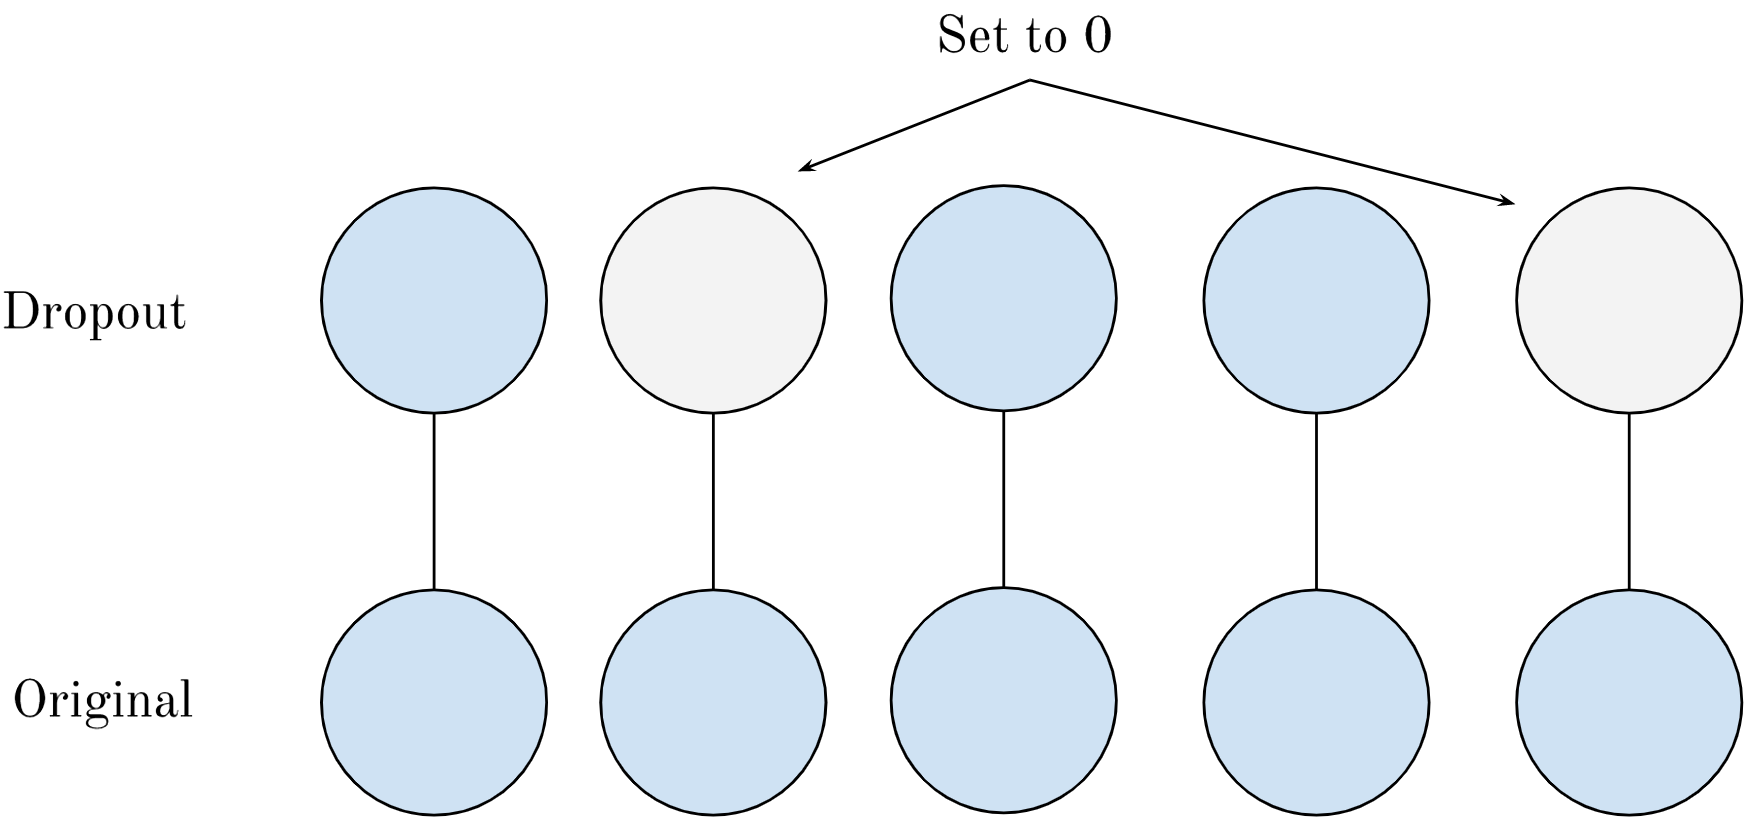
\includegraphics[width=0.85\textwidth]{graphics/dropout.png}
	\caption{Certain neurons are set to 0 (dropped out) in a dropout layer \cite{Goodfellow-et-al-2016}}
	\label{fig:dropout}
\end{figure}

Due to the sheer amount of hyperparameter and possible approaches, successfully designing and training a neural network can be a challenging task \cite{anintroductiontoneuralnetworks}. There are many rules of thumbs for many hyperparameters but in the end it is in the hand of the developer to use a good mixture of clever tricks, as well as trial and error to find a good neural network model \cite{Goodfellow-et-al-2016}. Automated machine learning is also a very promising research field, more information is available at section \ref{transferlearning}.

The architecture of the neural network also influences how much it tends to overfit: As a rule of thumb, the more neurons a neural network has, the bigger the learning capacity of the neural network and the more easy it overfits if the dataset is not sufficiently large \cite{Goodfellow-et-al-2016}. Empirically deep networks (many layers) have shown to generalize better compared to less deep networks but with similar number of neurons \cite{Goodfellow-et-al-2016}.

\subsection{Backpropagation} \label{backprop}

Backpropagation is an alternative way of determining the gradient of a function \cite{Goodfellow-et-al-2016}. Backpropagation makes training big neural networks tractable for modern computers \cite{bishop}. Due to its useful properties backpropagation has been reinvented independently in several fields. \cite{Griewank2012WhoIT}. Backpropagation is also known as reverse-mode differentiation \cite{colahbackprop}.

\begin{figure}[ht]
	\centering
  	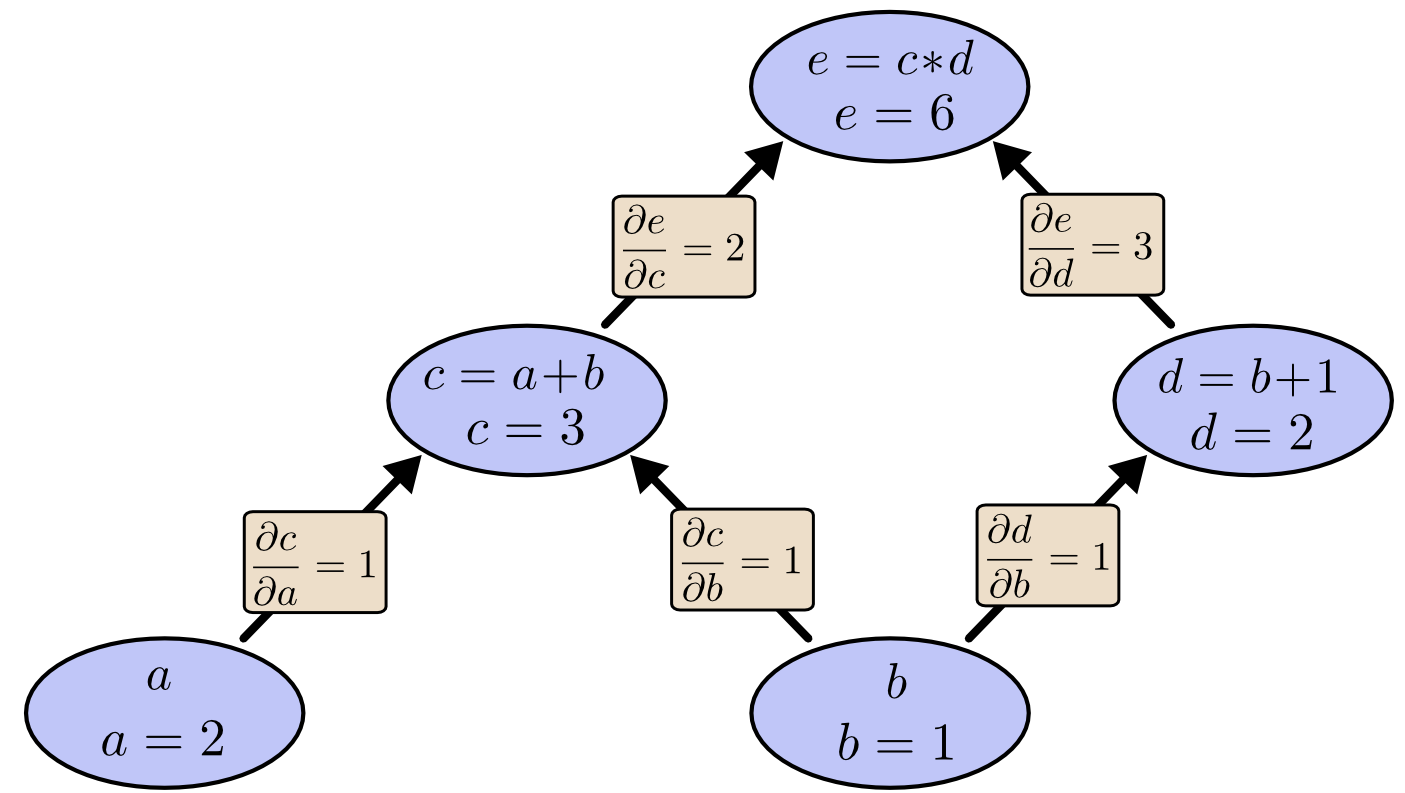
\includegraphics[width=0.75\textwidth]{graphics/computationgraph.png}
	\caption{A computational graph with derivatives on the edges. \cite{colahbackprop}}
	\label{fig:computationgraph}
\end{figure}


Another view of neural networks is the view of computational graphs \cite{Goodfellow-et-al-2016}. Neural networks essentially define a graph of simple computations consisting of differentiable operations \cite{Goodfellow-et-al-2016}. In a computational graph derivatives are placed on the edges between nodes. Figure \ref{fig:computationgraph} illustrates a computational graph.

Calculating the derivative of $e$ with respect to $b$ in the graph illustrated in figure \ref{fig:computationgraph} can be calculated by summing over all paths in the computational graph \cite{colahbackprop}:

\begin{equation}
\frac{\partial e}{\partial b} = 1 * 2 + 1  * 3
\end{equation}

\begin{figure}[ht]
	\centering
  	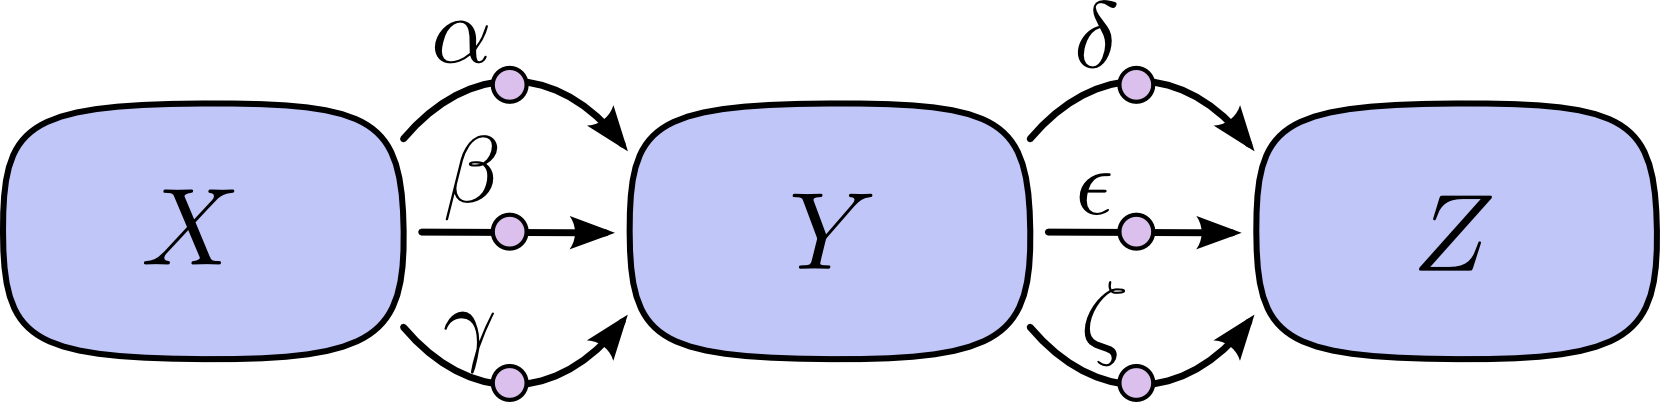
\includegraphics[width=0.75\textwidth]{graphics/computationgraphsimple.png}
	\caption{A simple computational graph \cite{colahbackprop}}
	\label{fig:computationgraphsimple}
\end{figure}

Summing over all paths quickly explodes combinatorially, as the number of paths may increase exponentially with the size of the graph \cite{colahbackprop}. For example applying traditional forward-mode differentiation ($\frac{\partial}{\partial X}$) the computational graph illustrated in figure \ref{fig:computationgraphsimple} would result in the following derivative \cite{colahbackprop}:

\begin{equation}
\frac{\partial Z}{\partial X} = \alpha \delta + \alpha \epsilon + \alpha \zeta + \beta \delta + \beta \epsilon + \beta \zeta + \gamma \delta + \gamma \epsilon + \gamma \zeta
\end{equation}

which could be greatly simplified instead by using backpropagation ($\frac{\partial Z}{\partial}$) instead:

\begin{equation}
\frac{\partial Z}{\partial X} = (\alpha + \beta + \gamma)(\delta + \epsilon + \zeta)
\end{equation}

Backpropagation starts at the output node and works towards the root nodes by calculating the derivative of $\frac{\partial Z}{\partial}$ \cite{colahbackprop}. Figure \ref{fig:computationgraphreverse} outlines backpropagation on a computational graph. Additionally this process also returns a derivative with respect to the output for every node in the graph \cite{Goodfellow-et-al-2016}. This is a very useful property for training neural networks \cite{Goodfellow-et-al-2016}.

\begin{figure}[ht]
	\centering
  	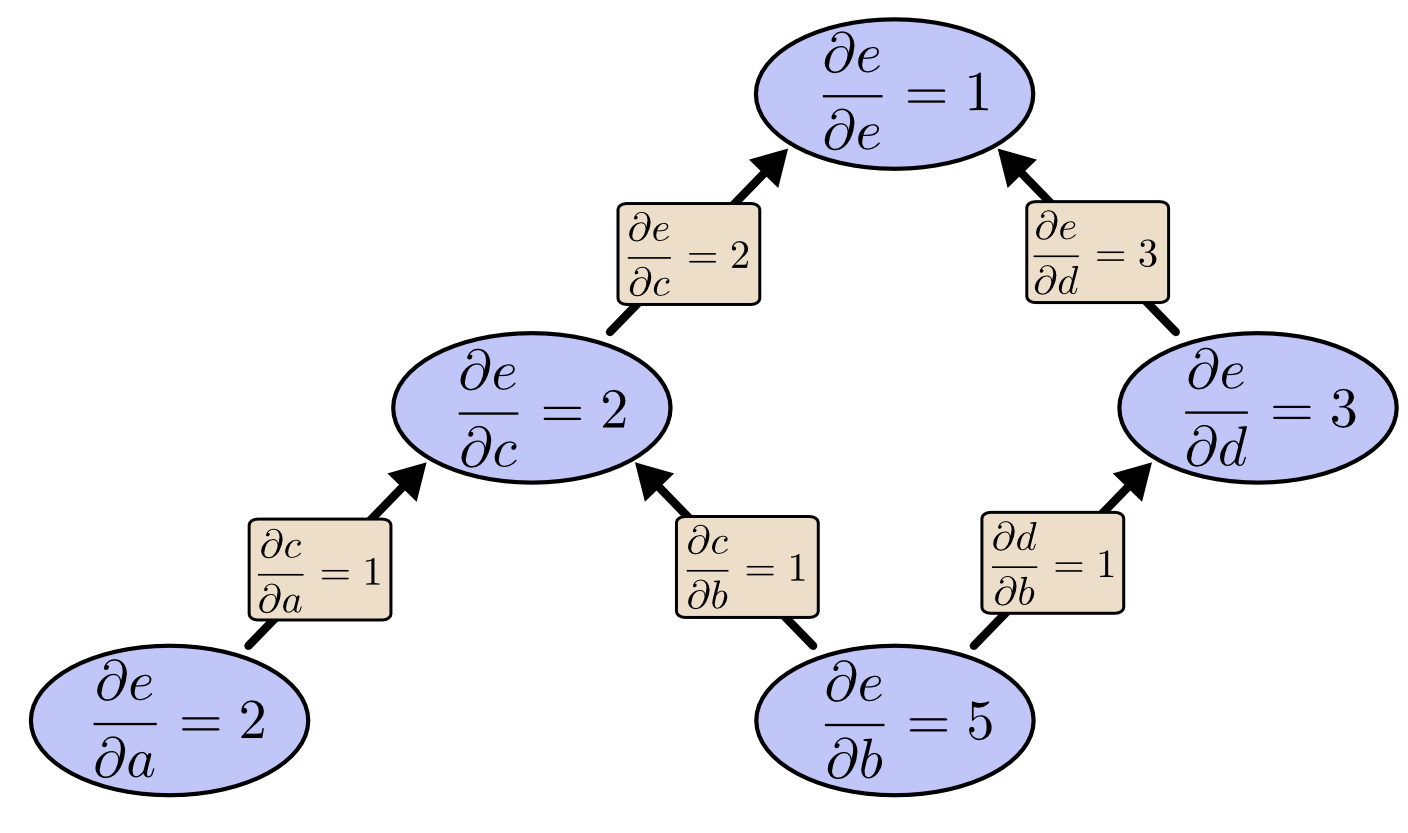
\includegraphics[width=0.75\textwidth]{graphics/computationgraphreverse.png}
	\caption{Backpropagation applied on computation graph \ref{fig:computationgraph} \cite{colahbackprop}}
	\label{fig:computationgraphreverse}
\end{figure}

Backpropagation can be summarized using the following pseudo code described at algorithm \ref{backpropalgo}.

\begin{algorithm}
\caption{Backpropagation algorithm \cite{dlvc}}

\ForEach{node n} {

Compute local gradient $l_c = \frac{\partial n}{\partial c}$ for each child $c$

Compute $m_c = l_c  \frac{\partial e}{\partial n}$ for every child $c$

Compute $\frac{\partial e}{\partial c}$ by summing over all $m_c$

}
\label{backpropalgo}
\end{algorithm}

\if false
Seiten: 1
\begin{itemize}

\item Momentum in Gradient Descent erklären
\item Minibatching erklären: Wieso? Effizienter Trainieren, weniger lokale extrema, schwierig richtigen wert für hyperparameter zu finden
\item Backpropagation erwähnen, aber nicht zur sehr ins Detail
\item Overfitting bekämpfen: Dropout, Regularisierung, Data Augmentation, Early Stopping
\item Wie Hyperparameter tunen? Faustregeln, Erfahrung, Trial'n Error
\item Architektur wichtig: Tiefe neuronale netzwerke sind im Allgemeinen besser als weite

\end{itemize}
\fi

\subsection{Deep Learning} \label{dlbackground}

A neural network with multiple layers, where each layer applies increasingly higher level feature extraction is a deep neural network \cite{deeplearninginneuralnetworks}. The research field is called deep learning \cite{deeplearninginneuralnetworks}.

An advantage of deep neural networks is that they scale very well with the size of the dataset and with the amount of computation power available \cite{alexnet}. As the computational resources increase and the size of the datasets as well, the performance of models deep learning enables also increases.

The technique of using multiple layers in neural networks has been around for many years \cite{deeplearninginneuralnetworks}. Relatively recently (2012), the field of deep learning has gained a lot of attention, since the introduction of AlexNet \cite{alexnet} as this was one of the first practical deep neural network outperforming more traditional methods \cite{deeplearninginneuralnetworks}. As the basic techniques of deep learning have been around for many years, the exorbitant computational requirements were still unsolved for many years \cite{deeplearninginneuralnetworks}. Deep learning on a conventional central processing unit is infeasible for large models \cite{deeplearninginneuralnetworks}. Emerging general purpose programming of graphics cards solved this problem: The training of deep neural networks can be very effectively parallelized and graphics cards excel at such tasks compared to CPUs \cite{Goodfellow-et-al-2016}. Training neural networks requires to compute the gradient of a large function \cite{Goodfellow-et-al-2016}. The gradient can be efficiently calculated using backpropagation \cite{aimodern}. %Backpropagation uses the chain rule to reuse interim results, akin to dynamic programming.

Despite backpropagation and large datasets, controlling the number of weights and biases is still an important factor of successful deep learning models \cite{deeplearninginneuralnetworks}. There are many types of layers, which essentially all serve to reduce the number of parameters \cite{Goodfellow-et-al-2016}. For example, convolutional layers are especially suited for image related tasks, as they have a relatively small number of parameters, but work much better than a comparable fully connected layer \cite{deeplearninginneuralnetworks}. More about convolutional neural networks in section \ref{mlcnn}.

A problem of neural networks and deep neural networks in particular is the lack of interpretability \cite{interpretabledl}. For humans it is very difficult to make founded assertions of what the neural network actually uses for its prediction \cite{interpretabledl2}. Neural networks are essentially black boxes with input on one side of the network and some prediction returned at the other side of the network \cite{interpretabledl}. This is especially a problem of safety critical systems, such as self-driving cars \cite{selfdriving}. In this domain it is critical for humans to know on which basis the system has decided and whether it is sensible. Natural language processing is also prone to such "clever hans" behaviour, where the neural network exploits statistical cues of the underlying data, instead of really understanding the task \cite{cleverhans}. Interpretable deep learning is an active field of research \cite{interpretabledl}.

\if false
Seiten: 1
\begin{itemize}
\item Was ist ein DNN? Unterschied zu MLPs.
\item Geschichte von Deep Learning. Wieso nicht schon früher? (GPUs und große Datenmengen!)
\item Wieso ist Backpropagation wichtig für DNNs? => Da mit forward propagation zu rechenaufwändig ist.
\end{itemize}
\fi

\subsection{Convolutional Neural Networks} \label{mlcnn}

\begin{figure}[ht]
	\centering
  	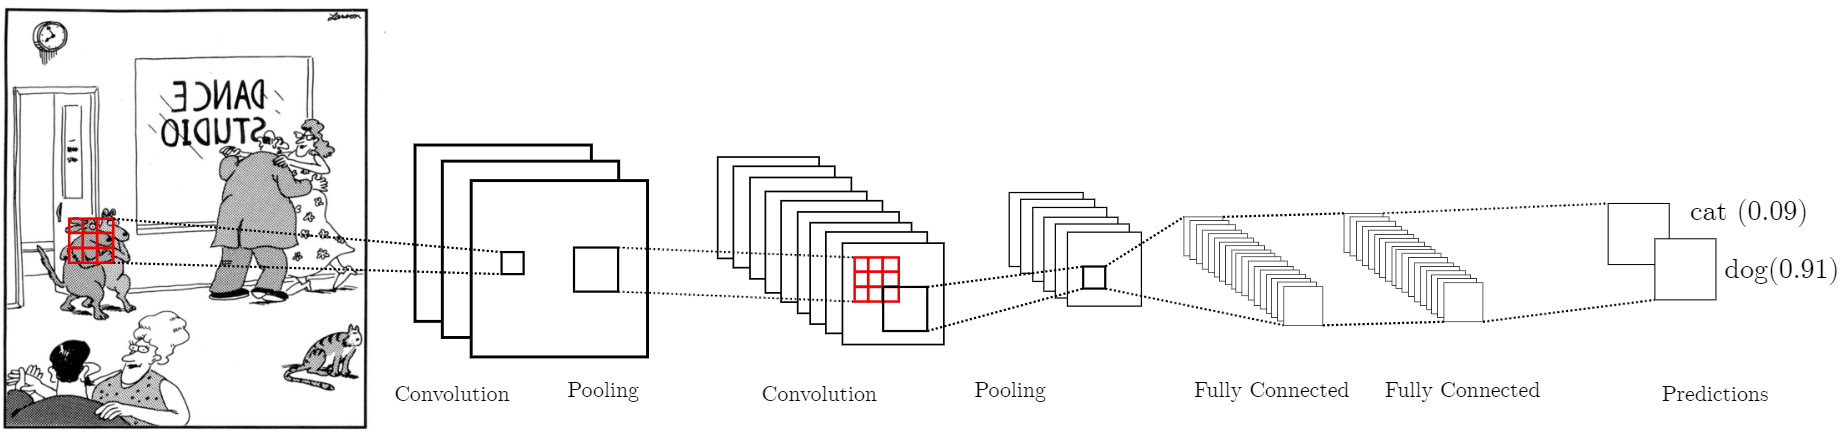
\includegraphics[width=1.0\textwidth]{graphics/cnn.png}
	\caption{Visual representation of a convolutional neural network}
	\label{fig:cnn}
\end{figure}

Based on feedforward neural networks convolutional neural networks emerged \cite{bishop}. A convolutional neural network (CNN) is a deep neural network \cite{alexnet}. The basic layer types of CNNs are: fully connected hidden layers, convolutional layers and max-pooling layers \cite{Goodfellow-et-al-2016}. Figure \ref{fig:cnn} illustrates an overview of the architecture of a convolutional neural network.

\begin{figure}[ht]
	\centering
  	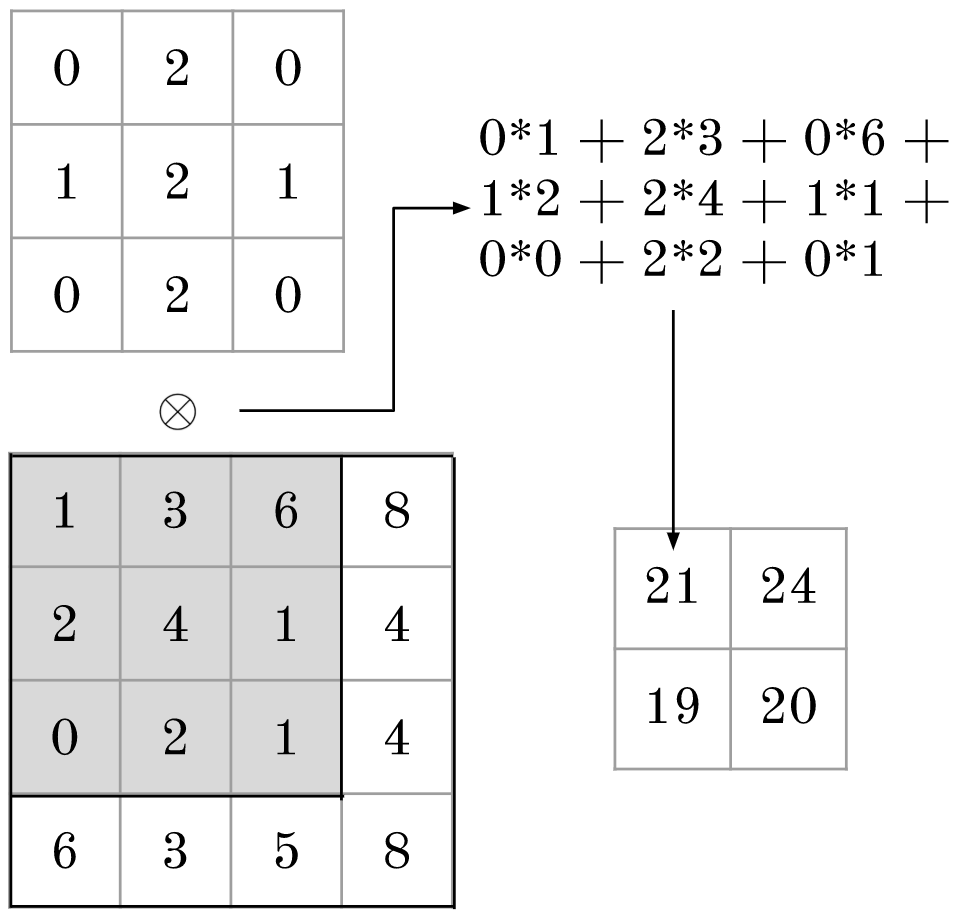
\includegraphics[width=0.5\textwidth]{graphics/convolution.png}
	\caption{3x3 convolution with stride=1 and no padding.}
	\label{fig:convolution}
\end{figure}

Convolutional layers apply a convolution on each pixel \cite{bishop}. A convolution is a weighted sum between two functions \cite{Goodfellow-et-al-2016}. The first function is the input signal and the second function a filter kernel \cite{bishop}. Instead of each neuron being connected to all other neurons, they are connected to a relatively small local subset of the neurons in the previous layer, which allows the layer to recognize certain local patterns (for example: edges) \cite{Goodfellow-et-al-2016}. The kernel is shared among the input neurons (parameter sharing) \cite{bishop}. This has two main advantages: It introduces translation invariance, which means that it does not matter if a feature occurs at the center or on near the edges of an images \cite{Goodfellow-et-al-2016}. Also it reduces the number of learned parameters significantly \cite{bishop}. Additionally to increase the capacity, multiple convolutions are applied per layer \cite{Goodfellow-et-al-2016}. This is called the depth of a convolutional layer \cite{Goodfellow-et-al-2016}. Due to their design, in contrast to fully connected layers, convolutional layers do not require a fixed input size, which means that they can be applied on images of different sizes \cite{dlvc}. The kernel has a size, which is usually $n$x$n$ \cite{alexnet}. To avoid the size reduction of standard convolutions, one can set the padding parameter of a convolutional layer \cite{Goodfellow-et-al-2016}. This increases the input data synthetically (for example by introducing a border with constant value). There is also a stride, which defines how the filter moves along the input \cite{Goodfellow-et-al-2016}. If the stride is fractional ($1/s$), it is also called a deconvolution or transposed convolution \cite{dlvc}. This operation increases the output size \cite{Goodfellow-et-al-2016}.


\begin{figure}[ht]
	\centering
  	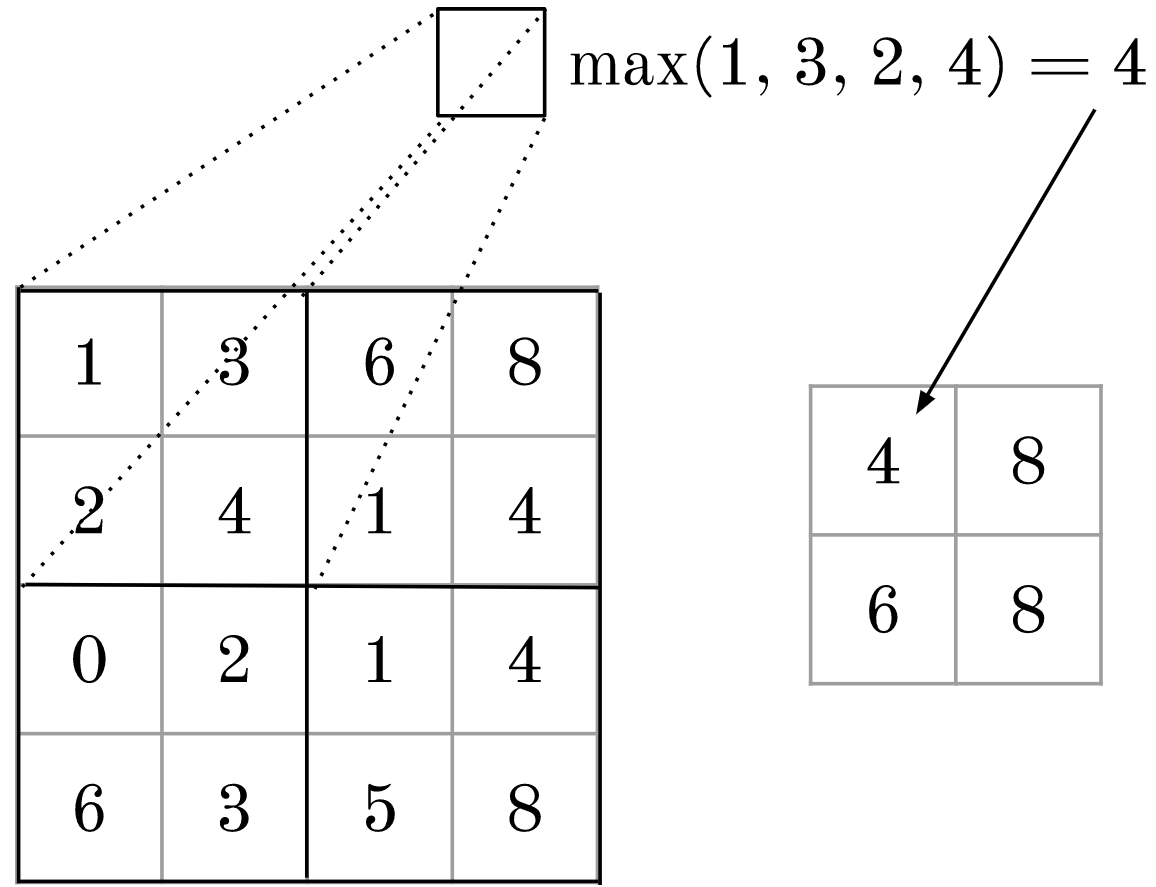
\includegraphics[width=0.5\textwidth]{graphics/maxpooling.png}
	\caption{2x2 max pooling of a simple 4x4 input layer into a 2x2 output layer}
	\label{fig:maxpooling}
\end{figure}

Pooling layers are applied after convolutional layers \cite{alexnet}. Their goal is to reduce the dimensionality of the data (as well as sometimes translational invariance) \cite{dlvc}. Local pooling layers are connected to a local subset of the neurons in the previous layer \cite{Goodfellow-et-al-2016}. The input is transformed by some function \cite{dlvc}. A typical pooling layer is max pooling, where the result is the maximum value of all incoming connections of the current local subset (for example 2x2) \cite{Goodfellow-et-al-2016}. Figure \ref{fig:maxpooling} illustrates a max-pooling operation. Another common type of pooling is average pooling \cite{Goodfellow-et-al-2016}. Another form of pooling is global pooling, where the entire data is pooled at once, this is usually applied at the end of the convolutional part of a CNN \cite{Goodfellow-et-al-2016}. Pooling does not involve learning weights, as the function applied is fixed before training \cite{Goodfellow-et-al-2016}. There are also problems associated with pooling, as it essentially makes the model forget information \cite{resnet}. This is one reason, why many modern convolutional neural network architectures mostly avoid max-pooling. \cite{resnet}

Fully connected layers are usually the last layers of a CNN, their task is to perform classification based on the extracted features of the previous layers \cite{alexnet}. Interestingly the convolutional part of a CNN can be used for another tasks with good performance, more about this at section \ref{transferlearning} \cite{deeplearninginneuralnetworks}.

\if false
Seiten: 1
\begin{itemize}

\item Erklärung was ein CNN ist
\item Illustration eines CNNs
\item Erklärung was eine Convolution ist
\item Illustration einer COnvolution
\item Erklärung was Max Pooling ist
\item Illustration von Max Pooling
\item Fully Connected Layers am Ende


\end{itemize}
\fi

\subsection{Recurrent Neural Networks} \label{lstmbackground}

\begin{figure}[ht]
	\centering
  	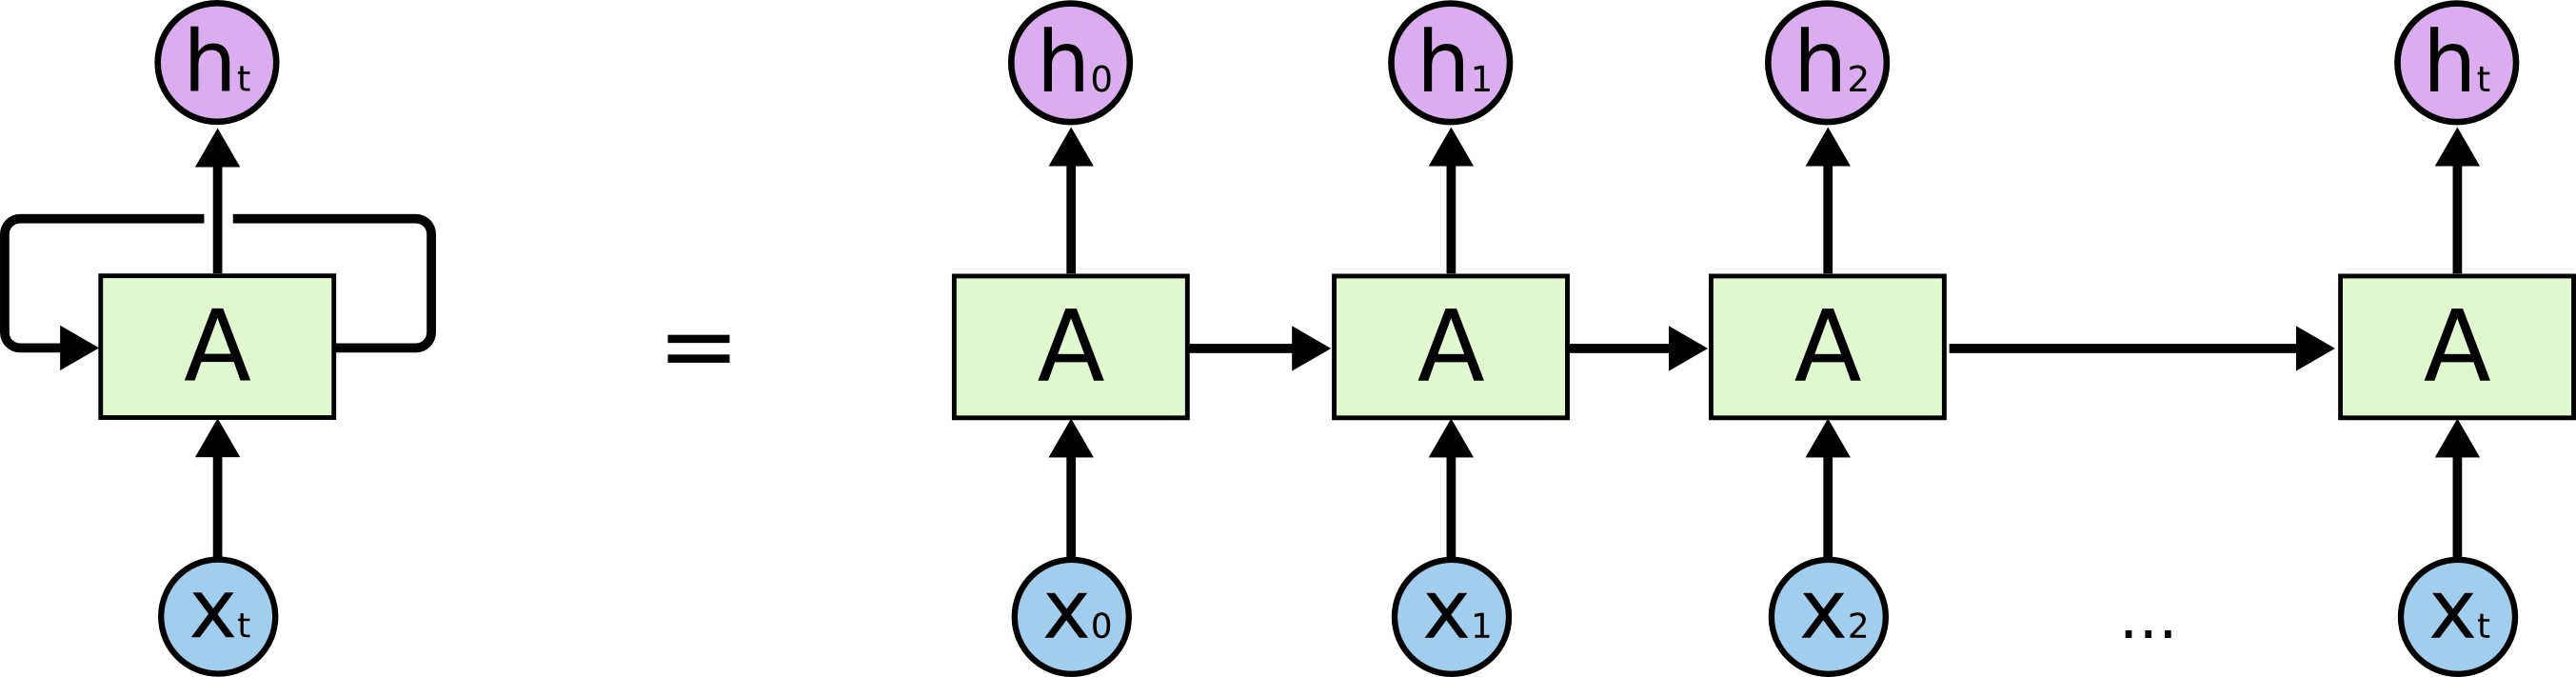
\includegraphics[width=1.0\textwidth]{graphics/rnn.png}
	\caption{Unrolling of a simple RNN cell over time \cite{colahlstm}}
	\label{fig:rnn}
\end{figure}

Recurrent neural networks (RNNs) are suited for sequences of arbitrary length, in contrast to normal fixed length input vectors for conventional feed forward neural networks \cite{hochreiter}. Recurrent neural networks are recurrent in the sense, that they contain cycles in the topology of the network  \cite{deeplearninginneuralnetworks}. In theory RNNs should be capable of understanding long-term dependencies \cite{hochreiter}. But naive RNNs with simple loops are not suited for longer sequences, because of the vanishing/exploding gradient problem \cite{hochreiter}. More about this problem is available in the original LSTM paper of Hochreiter et al \cite{hochreiter}. Figure \ref{fig:rnn} shows how unrolling of recurrent connections into a network without loops can be performed. This process converts  recurrent neural networks into feed-forward networks when applied on a sequence.

Replacing the naive approach with Long Short-Term Memory (LSTM) cells has shown to be successful for many tasks \cite{nmt}\cite{hochreiter}\cite{deeplearninginneuralnetworks}. A newer approach to this problem are gated recurrent units (GRUs) \cite{gru}.

Among LSTM/GRU cells there are many variations \cite{Goodfellow-et-al-2016}. Empirically GRUs have shown to train faster, but no significant difference regarding performance has been observed in general \cite{gru}.

The simplest LSTM unit consists of a memory cell with input and output gates \cite{hochreiter}. Inside the LSTM is a self-recurrent connection, which keeps the vanishing/exploding gradients inside the cell \cite{hochreiter}. For an illustration of an LSTM, refer to figure \ref{fig:lstm}.

\begin{figure}[ht]
	\centering
  	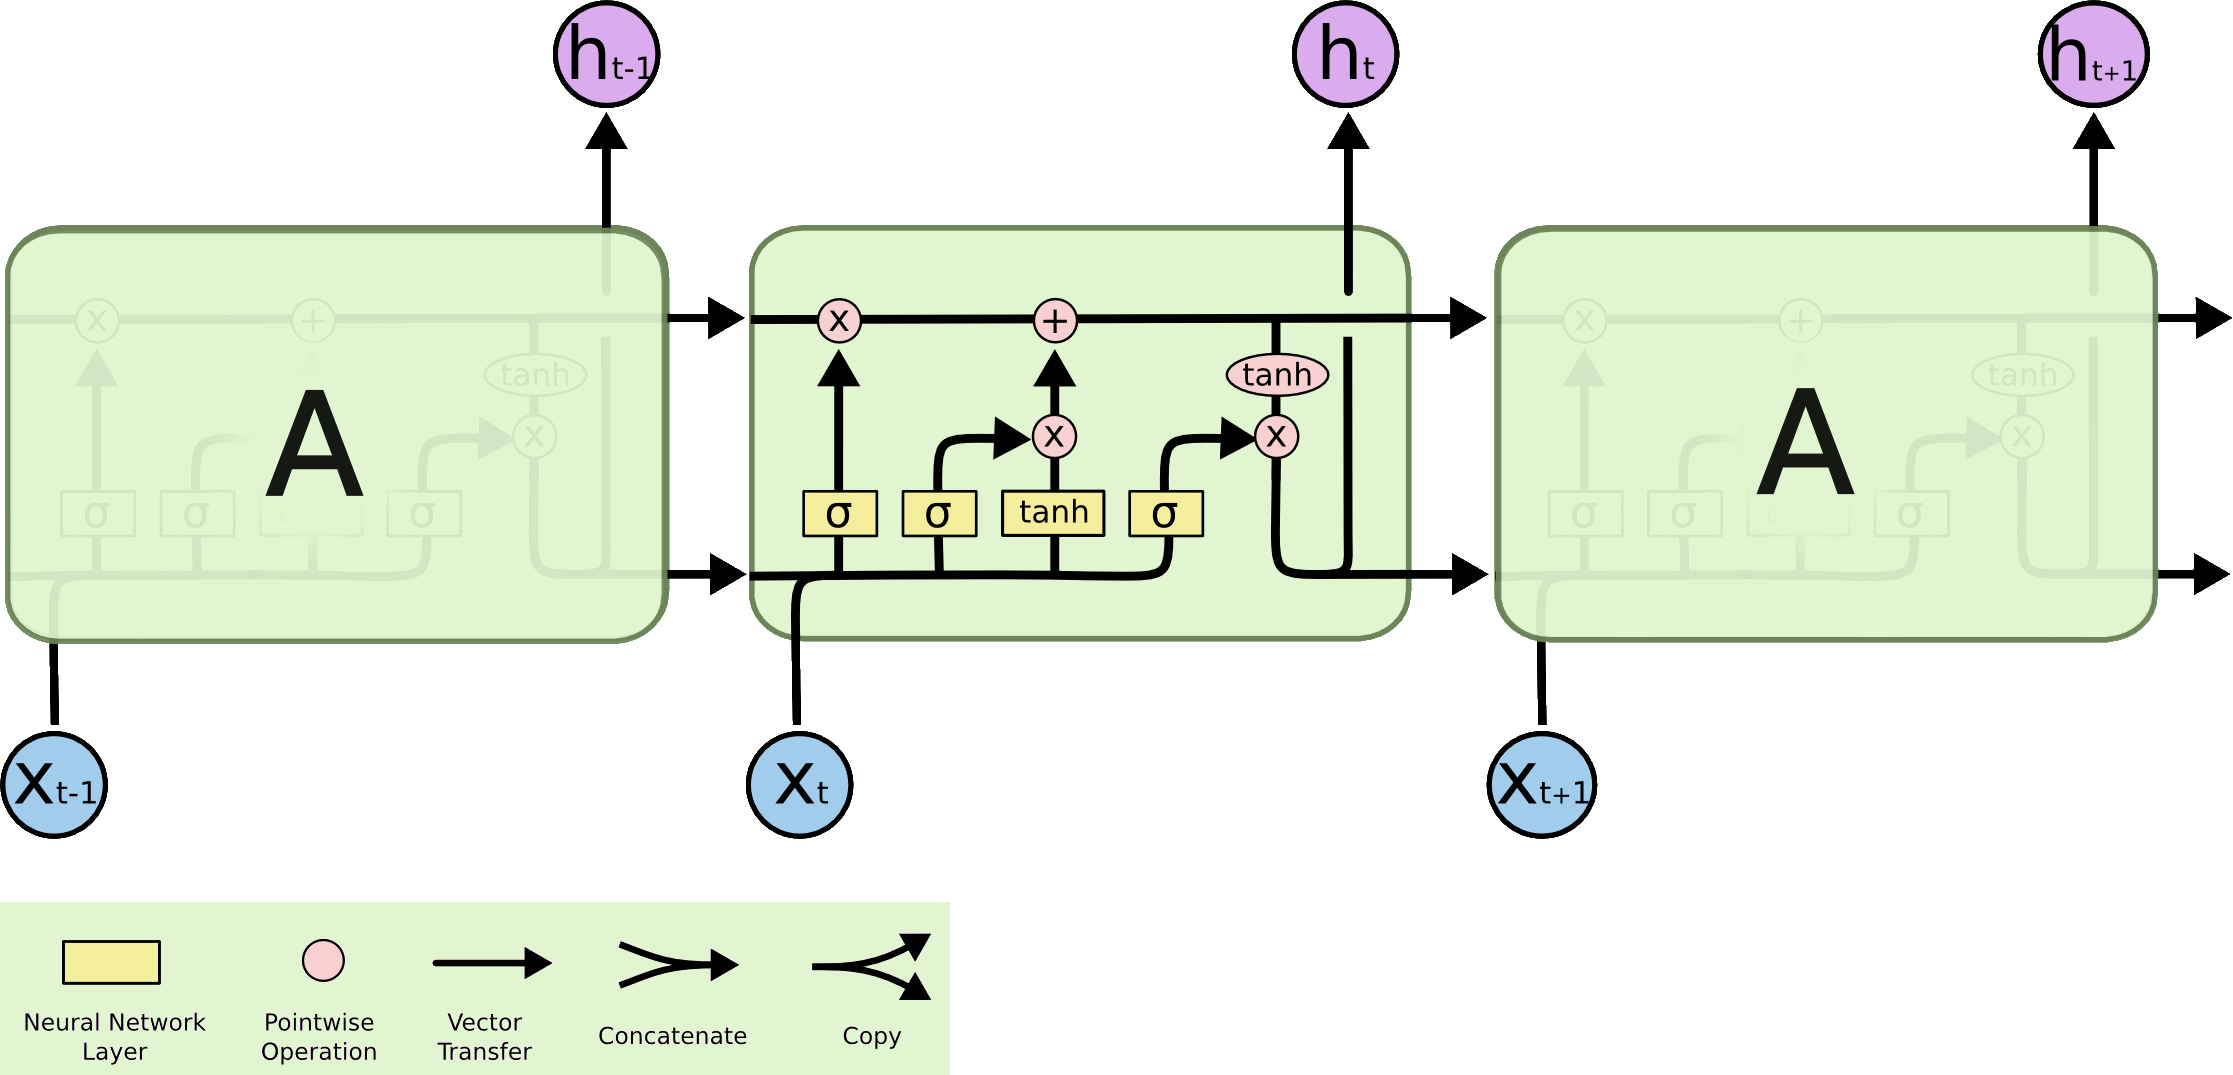
\includegraphics[width=1.0\textwidth]{graphics/lstm.png}
	\caption{Overview of an LSTM \cite{colahlstm}}
	\label{fig:lstm}
\end{figure}



\if false
Seiten: 1
\begin{itemize}

\item RNNs erklären (NNs mit Loops)
\item Illustration eines RNNs
\item Problem mit RNNs: Vanishing Gradient erläutern
\item LSTMs und GRUs referenzieren
\item Illustration einer LSTM Zelle

\end{itemize}
\fi


\subsection{Autoencoder}

\begin{figure}[ht]
	\centering
  	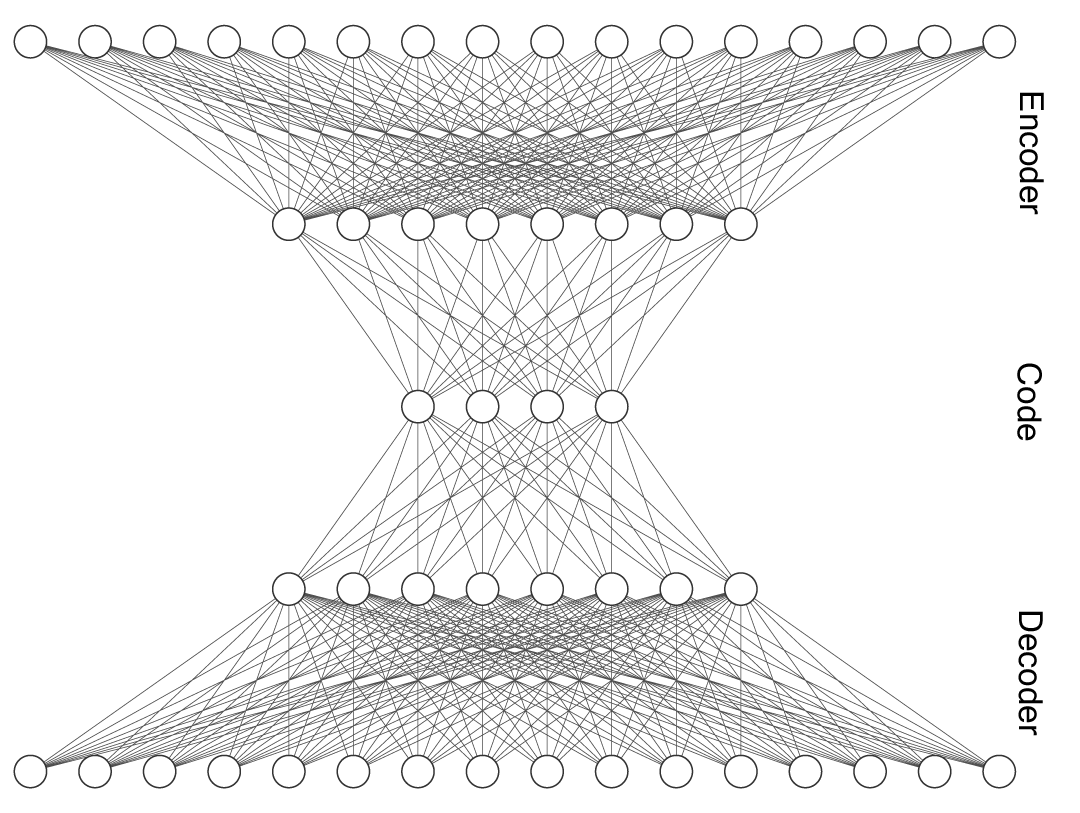
\includegraphics[width=1.0\textwidth]{graphics/autoencoder.png}
	\caption{A fully connected autoencoder with 2 encoding and 2 decoding layers}
	\label{fig:autoencoder}
\end{figure}

An autoencoder is a deep neural network which learns a compact representation of data without supervision \cite{Goodfellow-et-al-2016}. This is similar to principal component analysis of traditional machine learning \cite{bishop}. An autoencoder consists of two parts \cite{Goodfellow-et-al-2016}: 

\begin{itemize}
\item Encoder: Performs a dimensionality reduction from a high dimensional data to a low dimensional representation \cite{Goodfellow-et-al-2016}
\item Decoder: Tries to reconstruct the original data from the low dimensional representation \cite{Goodfellow-et-al-2016}
\end{itemize}

For example, an autoencoder architecture can be used to reduce the dimensionality of images while still preserving important semantic information. Figure \ref{fig:autoencoder} shows a simple fully connected autoencoder. As CNNs perform very well in the image domain, they are a natural fit for autoencoders for images \cite{cnnimg}. The encoders consists of standard convolutional blocks (convolution + max pooling). While the decoder has to restore the original image, therefore it usually consists of layers performing a transposed convolutions \cite{dlvc}. 

\if false
Seiten: 0.5
\begin{itemize}
\item Zweck von Autoencoder erläutern (Dimensionality Reduction, ähnlich wie PCA)
\item Illustration eines Convolutional Autoencoder
\item Encoder/Decoder erklären.
\end{itemize}
\fi

% SUM: 13.5-14

\section{Natural Language Processing} \label{nlpbackground}

Natural Language Processing (NLP) combines the disciplines of artificial intelligence and linguistics \cite{statisticalnlp}\cite{speechandlanguageprocessing}. NLP researchers try to build computer programs capable of understanding human language \cite{speechandlanguageprocessing}. Common tasks of NLP include part-of-speech tagging, paraphrase identification, machine translation and speech recognition \cite{surveynlp}\cite{nmt}\cite{googlespeech}\cite{speech}\cite{paraphrase}.

Early NLP tried to achieve its goal by building traditional parsers, similar to what compilers do for programming languages \cite{speechandlanguageprocessing}. Unfortunately, these techniques are inadequate for human languages, due to the ambiguity of human language \cite{statisticalnlp}.

Another common approach has been to apply traditional machine learning for NLP \cite{statisticalnlp}. The general approach is to extract certain features of a text corpus and use these features to train a classical machine learning model \cite{svmnlp}. Empirically, the best performing machine learning algorithm for this context are support vector machines \cite{svmnlp}.

Deep learning currently achieves many state-of-the-art results in NLP \cite{nmt}\cite{paraphrase}. An advantage of many text problems, is the abundance of large corpora, partly due to the rise of the internet \cite{bert}. This is an important advantage especially for unsupervised methods, since labelling of large corpora may be very expensive \cite{elmo}\cite{bert}.

For both traditional machine learning and deep learning based natural language processing it is important to extract the right features from the dataset \cite{statisticalnlp}. High level features (sentence length) are usually not sufficient, therefore the sentences must be converted into more useful features \cite{Yang2015HumorRA}.

A trivial approach would be to give each word a unique identification number \cite{deeplearningnlpstanford}. This approach does not grasp important semantic information about the words \cite{deeplearningnlpstanford}. For example, the words king and queen are more similar than king and house. If the featurization assigns the ID=2 for king and the ID=42 for queen, then the machine learning model has no additional information, that these words are similar concepts. Keeping this information is crucial for successful natural language processing \cite{nmt}\cite{elmo}. Vector space models avoid this problem by representing each word in a high dimensional vector space, where a certain similarity measure holds \cite{pennington2014glove}.

There is the concept of positive and negative similarity \cite{TUW-233295}. Positive similarity is denoted using the $\otimes$ operator. Negative similarity is denoted using the $\overline{\otimes}$ operator \cite{TUW-233295}. Similarities based on the dot product are positive similarity measures \cite{TUW-233295}. The cosine similarity is a commonly used positive similarity measure \cite{modernir}. While similarities based on distance (for example: euclidean distance) are negative similarity measures \cite{TUW-233295}. CNNs are based on positive similarity: They perform a convolution, which is also a positive similarity measure \cite{alexnet}. Vector spaces have usually several 100 dimensions \cite{bert}. Positive similarity measures perform empirically better on high dimensional spaces compared to negative similarity measures \cite{surprisinghighdimensional}. Vector space models can be seen as a form of word embeddings \cite{elmo}.

\if false
Seiten: 1.5
\begin{itemize}
\item Was ist NLP: Aus welchen Subdisziplinen besteht es (AI, Linguistik)
\item Ziel von NLP
\item Geschichte von NLP (Parser => SVM => Deep Learning)
\item Feature Extraction in NLP => Word Embedding
\item Wieso Word Embedding? Weil, ID keine semantische Information enthält => Vektor sollte deskriptiv sein
\item Vector Space Model erklären
\item Similarity (Positive vs. Negative Similarity). Bezug zu Convolution herstellen
\end{itemize}

\fi

\subsection{TFIDF}


TFIDF stands for term frequency inverse document frequency and is a simple, but powerful vector space model. The idea originated in information retrieval, where the goal was to weight words by their importance for a document and for a query. The TFIDF consists of two frequencies multiplies: Term frequency and inverse document frequency. The term frequency (TF) describes the total number of times a word occurs in a document. The idea being, that the more often a word occurs, the more important it is in describing the document.

The problem with this is that certain words occur almost always very frequently (stop words). For example, the word "the" would have almost always a very high term frequency, but is rarely important for describing the document. This is the reason why the inverse document frequency (IDF) is also considered. This weight describes the importance of a word compared to all other documents. For example, a document about the Engima machine would have frequent mentions of the word "Engima", therefore the IDF would be relatively high compared to other words. In contrast, the word "the" occurs usually in all documents, therefore the IDF would be very low.

There exist many different formulas which entail this idea. In this thesis the following TFIDF equations were used:

\begin{equation}
\text{idf}(t) = \text{log} \left(\dfrac{n}{\text{df}(t)} \right) + 1
\end{equation}
\begin{equation}
\text{tfidf}(t, D) = \text{tf}(t, D)idf(t)
\end{equation}


where $t$ is some term, $D$ some document, $\text{tf}(t, D)$ the number of occurrences of term $t$ in document $D$ and $\text{df}(t)$ the number of documents containing term $t$.

The advantage of TFIDF is, that is very easy to understand and does not need any time consuming training, as it only counts word occurrences. This makes it very feasible to be trained locally, without the need of any pretrained model. The main disadvantage is that TFIDF does not capture the context of the word well. It is a bag-of-word approach which ignores the word order completely.

\if false
Seiten: 0.75

\begin{itemize}
\item Definition von TFIDF. 
\item Intuitive Erklärung
\item Formel
\item Vorteile / Nachteile von TFIDF
\end{itemize}

\fi

\subsection{GloVe \cite{glovepage}}
The basis for training GloVe is a word to word matrix which denotes the frequency of words occurring together in the training data. The intuition of this word embedding is that the ratios of word-word co-occurrence may encode the underlying meaning of the words. During training of the model the objective is to learn word vectors such that the dot product equals to the logarithm of the probability of co-occurring with another word.

GloVe is also a bag-of-word approach, as it uses a word to word matrix without any information about sequence.

For a more detailed explanation please refer to the introductory paper \cite{glovepage}.

\if false
Seiten: 0.25

\begin{itemize}
\item Was ist GloVE?
\item Intuitive Erklärung
\item Detailierte Beschreibung mit verweis auf Paper
\end{itemize}

\fi

\subsection{ELMo \cite{elmo}}
Previous models have very limited sense of context, especially each word had the same word vector associated regardless of the context. ELMo (Embeddings from Languages Models) assigns word embeddings depending on context.

First a language model has to be trained for ELMo. A language model enables to predict the next word given a sequence of prior words. For example given the sequence of words "Yesterday I was in New York. I visited the statue of ...", a good language model could predict that the next word would be "Liberty".

ELMo models language using a 2-layer bidirectional LSTM with residual connections, which allows training of deep models more efficiently. However the words still must be converted into a vector representation. This is achieved by first converting the words into a character embedding and then a convolutional layer with max-pooling is applied. The character embedding has the advantage that the model handles words which are not in the vocabulary better.

The novel idea of ELMo is not how it is trained, but how the trained language model is applied: ELMo calculates the final word embedding for a word by combining the different hidden states of the LSTMs and the output of the convolutional part into a unified vector representation. The combination is done by multiplying a weight to each state, which is also learned.

This is a short summary of a relatively complex architecture. For more details the work of Gardner et al is recommended. \cite{elmo}

\if false
Seiten: 0.5

\begin{itemize}
\item Was ist ELMo
\item Intuitive Erklärung der Architektur (Training)
\item Besonderheit von ELMo (nicht wie es trainiert wird, sondern wie es verwendet wird)
\end{itemize}

\fi


\section{Transfer Learning} \label{transferlearning}

Usually, the more complex a given task is, the more labelled data deep learning needs to achieve good results. This is not only expensive, but sometimes not possible. For example, Gary Larson has only drawn so many cartoons in his lifetime. Labelling a big dataset is also a big challenge and not always feasible.

Transfer learning tackles this problem: Instead of training a completely new model for each problem task, the idea is to reuse models and only slightly adapt them for new tasks. The original model is trained on an already existing big dataset and the dataset of the fine tuning can be orders of magnitudes smaller. This tuning in the context of deep neural networks is usually done by fixating the weights of neurons in certain higher layers during training. Usually lower layers perform more general feature extraction, which can be transferred to other domains more easily.

For example there are already very big datasets for image classification tasks. Training a good performing classifier on these datasets has already been done numerous times. Especially CNNs have an architecture very suited for transfer learning: As mentioned in [\ref{mlcnn}], there is the convolutional part and the fully connected part. Usually the convolutional part is acting as a feature extractor and the fully connected part makes the final prediction. Empirically it has been shown that the feature extractor generalizes often very well to new domains. Depending the similarity of the domains, less training is needed for the new domain. For example, this thesis uses a pretrained ResNet8 model which has very good performance for traditional image classification tasks and applied it on Gary Larson's cartoons.

Natural language processing works similarly by transferring word embeddings between different corpora. Importantly these word embeddings transfer well for a broad range of tasks and still achieving state-of-the-art performance. \cite{elmo}


\if false
Seiten: 1
\begin{itemize}
\item Problem von klassischem Deep Learning (Große Datenmengen) erläutern
\item Mögliche Lösung des Problems: Transfer Learning => Model zuerst an Domain A trainieren und dann bei Domain B anwenden wobei |A| >> |B|
\item Transfer Learning mit Bildern erläutern => CNNs den Convolutional teil übernehmen und rest neu trainieren
\item Transfer Learning mti Text erläutern => Word Embedding (zB ELMo/BERT)
\end{itemize}
\fi


\section{AutoML} \label{automlbackground}

AutoML stands for automated machine learning and is the process of automated end-to-end training of machine learning models without the help of a human. Naive automated approaches such as grid search or random search have exponential runtime with increasing number of hyperparameters.

Grid search is a simple approach, where a model for possible combinations of hyperparameters is trained. Similarly random search assigns random hyperparameters until some halting criterion is reached.

Solving a problem using machine learning requires many non-trivial tasks, such as:

\begin{itemize}
\item Data pre-processing
\item Feature engineering
\item Feature selection
\item Algorithm selection
\item Hyperparameter selection
\end{itemize}

AutoML tries to automate all or a subset of these tasks. A human can only try several different hyperparameter configurations and pre-processing steps. Applying machine learning techniques to automate this process therefore has the chance to save much time and even result in possibly much better models.

\subsection{Hyperopt-Sklearn \cite{hyperoptpaper}}

This paper uses the automated machine learning algorithm implemented in the works of Komer et al \cite{hyperoptpaper}. Their philosophy is that the selection of the entire machine learning pipeline (including data pre-processing) can be seen as a single large hyperparameter optimization problem.

Using Hyperopt-sklearn requires the machine learning practitioner to define the following parameters (also known as hyper hyperparameters):
\begin{itemize}
\item Objective function: Mapping of a configuration into a scalar value, which the algorithm tries to minimize
\item Search domain: Random variables whose distribution should match the most likely best configuration 
\item Optimization algorithm: An algorithm which finds the best configuration in the search domain given the objective function
\end{itemize}


\if false
Seiten: 0.5

\begin{itemize}
\item Hyperparameter Tuning Problem: Großer Search Space
\item "Traditioneller" Approach erläutern (Grid Search, Random Search, Experterfahrung)
\item Exponentieller Suchraum => Wende AI Technik an um Hyperparameter zu tunen
\item Was kann alles durch AutoML optimiert werden (Hyperparameter, Data processing, etc.)
\end{itemize}

\fi

\section{Computational Humor} \label{comphumorbackground}

According to the Oxford dictionary humor is the "the quality in something that makes it funny or amusing; the ability to laugh at things that are amusing" \cite{humordef}. The exact reasons for why humans developed humor is still under debate. It seems, that humor contributes to physical and psychological well-being. \cite{humorhealthy} Evolutionary psychologists have proposed, that humor may have been a result of sexual selection: Women may have preferred men with humor, as it may have been a sign of intelligence, adaptability, and desire to please others. \cite{sep-humor}

Over the centuries, there many theories of humor have been proposed. From the superiority theory, where the idea is that laughter expresses feelings of superiority over other people (or a former self). This theory was popular until the 20th century. Another early theory popular in the 20th century is the relief theory, which proposes that humor can be seen as a valve which releases pressure. This pressure was proposed to be some kind of gas or energy. The incongruity theory proposes, that humor is the result of the perception of something incongruous. In particular if the mind observes something which violates our mental model and expectations. This is in line with many of Gary Larson's cartoons: The cartoon sets up some expectation, which is usually in contrast to what the reader would have expected. For example scientists behaving like toddlers in usually serious situations. \cite{sep-humor}

A more modern view of humor is seeing it as a form of play. It has been observed, that many animals learn important skills during play. Humor seems to serve a similar purpose for human social behaviour. Usually humor shows what should be avoided during communication or in other (social) situations. Laughing and smiling enables these situations and therefore can be considered as a signal to play. 

Computational humor combines the field of artificial intelligence and computational linguistics, with the goal of computers understanding humor. As the interface between humans and computer becomes more natural, it is also important that computers can also understand humor. The rise of chatbots and virtual assistants (for example Apples Siri or Amazons Alexa) shows that humor is still a very difficult task for these application, as most people who have used such a system can confirm.

One problem of humor is, that it is very subjective. There is no general humor, as every person finds different things funny. There are topics or types of humor that more people find funny than others. This is possibly the reason why there is currently no unified computational model of humor, instead models for certain subtasks of computational humor were built.

Common subtasks involve generative or discriminative tasks. An example for generative task would be joke generation or pun generation. In these kind of tasks the computer has to synthesize a joke or a pun. A discriminative task would be for example joke recognition. In this setting the computer should be able to detect whether some text is a joke or not.

Another challenge of computational humor is language understanding. To really understand a joke, the interpreter (be it human or computer) has to understand the language. Proper language understanding is still an important research topic. Until then, it is questionable whether computational humor will reach pass the Turing test.

Many early approaches of computational humor have focused on the incongruity theory, where humor is an unexpected difference between the expected and the unexpected. \cite{comphumorsummary} The general idea was to find or produce contradictions between what a human would expect and what has been communicated. These approaches had only limited success, since the underlying language understanding was not sophisticated enough. The computer did not have a proper model of what the human would understand and therefore could not apply the incongruity theory successfully.

Another problem was their heavy reliance on ontologies, such as WordNet and VerbNet. These are human crafted databases with concepts and their relationship to each other. The problem with these are the ambiguity of many concepts and also their limited size. For example VerbNet had only around 4500 verbs, which made it so that the computer had only a very limited understanding of the sentences. \cite{comphumorsummary}	


\if false

Seiten: 2
\begin{itemize}
\item Bedeutung von Humor (laut Oxford Dictionary)
\item Ursprung von Humor erläutern: Superiority Theory, Incongruity Theory, Humor als Spiel.
\item Computational Humor => kombiniert AI, Computational Linguistics
\item Problem von Humor: Subjektiv
\item Generativer Computational Humor: zB Witze erzeugen
\item Klassifizierender Computational Humor: zB Witze erkennen
\item Problem von Computational Humor: Language Understanding.
\item Ansätze für Computational Humor: Anwenden der Incongruity Theory und was die Probleme waren (https://ieeexplore.ieee.org/stamp/stamp.jsp?tp=\&arnumber=1613822)
\end{itemize}
\fi

% 20 Seiten

\section{Related work} \label{relatedworkbackground}

In this chapter I outline several works of the field of computational humor related to our work. Beginning with traditional approaches, which do not use deep learning. Then I will continue with deep learning based works.


\subsection{Computational Humor using Traditional Methods}

In the following sections we will discuss several works in the field of computational humor with traditional machine learning methods.

\subsubsection{Humor Recognition and Humor Anchor Extraction \cite{Yang2015HumorRA}}

This paper formalizes humor as a binary classification task between humorous and non-humorous. The authors perform their experiments on two datasets: Pun of the Day and One-liner dataset for positive examples and while samples for the negative class come from various other sources (Yahoo! Answers, New York Times, AP News and Proverb). The negative class samples are filtered, such that the sentences are approximately the same length and contain the same words as the positive class.

The authors extract several features from the input sentences that describe some aspect of humor.

\begin{itemize}
\item Incongruity Structure: Disconnection (maximum meaning distance of word pairs) and Repetition (Minimum meaning distance of word pairs)
\item Ambiguity Theory: Sense combination (the higher the more possible interpretations a sentence has), Sense Farmost (largest path similarity of any word senses) and Sense Closest (smallest path similarity of any word senses)
\item Interpersonal Effect: Negative (Positive) polarity (number of occurrences of negative (positive) words) and Weak (Strong) Subjectivity (number of occurrences of all weak (strong) subjectivity oriented words.
\item Phonetic Style: Alliteration (number and maximum length of alliteration chains) and Rhyme (number and maximum length of rhyme chains)
\end{itemize}

The work describes the training of a classifier based on above features. Important for the humor anchor extraction is the fact that all these features are word order independent and function also on partial sentences. Additionally to these human centric features the best performing model also uses Word2Vec features.

Humor anchor extraction is about extracting the key words that enable the humor of a sentence. Removing these words would make the sentence not humorous. The paper lists the example of the sentence "I used to be a watchmaker; it is a great job and I made my own hours" with a sensible selection of anchors "watchmaker", "made" and "hours".

The procedure of determining humor anchors is surprisingly simple. As the feature can be computed on any (partial) sentence the algorithm can freely remove words and still get a reasonable prediction. Also, only certain word types are considered (verbs, nouns, adverbs and adjectives). Pseudo code at \ref{humoranchorextraction} describes this algorithm on a high level.

\begin{algorithm}
\caption{Humor anchor extraction}\label{humoranchorextraction}

Take only verbs, nouns and adverbs of original sentence

Calculate humor score

\ForEach{$\text{possible anchor subset of sentence}$}{

Calculate humor score of subset

}

Return subset with maximum decrement

\end{algorithm}

From a performance point of view both the humour recognition seem to work well. On the Pun of the Day dataset the best model reaches an F1 score of 0.859. The One Liners dataset reaches an F1 score of 0.805.

Humor anchor extraction also performs quite well. The authors perform a quantitative evaluation by comparing 200 random samples that were annotated by three annotators. The strict variant, where the anchors must be exact reached an F1 score of 0.438 and an F1 score of 0.756 for the relaxed version where at least one word had to match on the Pun of the Day dataset. For the One Liners dataset the performance was worse: The strict version reaches an F1 score of 0.288 and an F1 score of 0.616 for the relaxed version.

\if false
Traditioneller Ansatz von Humor erkennung.

\cite{Yang2015HumorRA}

Seiten: 0.5


\subsubsection{Contextualized Sarcasm Detection on Twitter}
Sarkasmus Erkennung mit Machine Learning Techniken

\cite{Bamman2015ContextualizedSD}

Seiten: 0.5
\fi

\subsubsection{Humorist Bot: Bringing Computational Humour in a Chat-Bot System \cite{HumoristBot}}

This work implements humor detection and joke generation in the context of a chatbot. A chatbot is a software agent able to hold a conversation with a human. Humorist bot is able to generate humorous anecdotes and react to the users humorous messages by adjusting its avatar. A funny message not only affects the answer of the bot, but also changes its avatar to a laughing avatar.

Their chatbot uses a rather traditional AIML knowledge base with different answer sets:
\begin{itemize}
\item Set for general conversation
\item Set for humorous sentence generation
\item Set for humorous sentence recognition
\end{itemize}

AIML is an XML format which describes a set of possible answers that are matched using pattern matching.

\lstset{language=XML}
\begin{lstlisting}
<category>
    <pattern>How are you?</pattern>
    <template>I am fine, and you?</template>
</category>
\end{lstlisting}

The authors implemented humor detection by focusing on the following aspects of humor: 

\begin{itemize}
\item Alliteration: based on phonetic transcription
\item Antinomy: based on the antinomy relationships of WordNet 
\item Adult slang: based on a set of words classified as adult slang
\end{itemize}

They do not apply any machine learning techniques, but instead implement handcrafted rules. The authors implemented joke generation by combining several AIML rules.

Evaluation shows that recognition of humor achieves an accuracy of 66\% for 100 randomly sampled humorous samples, while a sample of 100 non-humorous sentences contained 19 false-positives. The authors did not perform an evaluation of the joke generation.


\if false
Traditioneller Ansatz in einem generativem Setting

\cite{HumoristBot}

Seiten: 0.5
\fi

\subsection{Computational Humor using Deep Learning}

In the following we will discuss the application of deep learning in the domain of computational humor. 

\subsubsection{Deep Learning of Audio and Language Features for Humor Prediction \cite{Bertero2016DeepLO}}

The work of Bertero et al compares several machine learning techniques for predicting and detecting humor in dialogues. They use a dialogue dataset of the series "Big Bang Theory", with annotations of canned laughter. Their goal is to predict these punchlines and where the canned laughter would appear. This work compares several techniques against each other: Convolutional neural networks, recurrent neural networks and conditional random fields. The convolutional neural network use low level representations of words and acoustic frames, while the other two methods use a set of acoustic and language features:

\begin{itemize}
\item Acoustic features: Extraction of pitch, Line spectral frequencies, intensity, loudness, probability of voicing, $F_0$ envelope, zero-crossing rate, MFCC and speaking rate features
\item Language features: Extraction of Lexical (unigrams, bigrams and trigrams appearing at least five times), structural and syntactic (proportions of verbs, nouns, adjectives and adverbs, sentence length and average word length), sentiment (average of positive/negative sentiment scores of SentiWordNet), Antonyms (presence of verb, noun, adjective and adverbs antonyms from WordNet compared to the previous utterance), Speaker turns (speaker identity) and Word2Vec features
\end{itemize}

Interestingly their work is not using an LSTM/GRU cell, but instead a simple RNN cell, which often have the problem of vanishing/exploding gradient. \cite{hochreiter} Their RNN architecture applies an embedding layer on the n-gram data and a separate embedding layer on the acoustic and language data for dimensionality reduction. Afterwards they combine both vectors and use this as an input for the RNN cell.

The CNN architecture uses two separate CNN branches for the sentence inputs and for the audio inputs. They use one convolution layer, with a sliding window of five tokens for the sentence input and sliding window of three frames for the audio input. Both branches have an embedding layer applied that reduces the dimensionality. After the convolutional layer, the authors apply a standard max pooling layer. Finally their implementation combines both CNN branches and global features into a single feature vector using a softmax layer.

Their corpus is split into a train/validation/test split, with 35865 utterances in the train set, 3904 utterances in the validation set and 3903 utterances in the test set. The corpus has in total 42.8\% punchlines.

The CNN shows to be the best performing approach to this task, as it reaches an F1-score of 68.5\%. RNNs performance is relatively low, which may be contributed to overfitting. Applying a LSTM/GRU cell would be an interesting experiment for future work. The authors themselves remarked, that Long Short-Term Memory cells will be evaluated in future work.

\if false
Deep Learning von Humor in Audiovisueller Domäne

Seiten: 1.0

\cite{Bertero2016DeepLO}
\fi

\subsubsection{A long short-term memory framework for predicting humor in dialogues \cite{bertero2016long}}

Bertero et al apply LSTMs on the same Big Bang Theory dialogue dataset as in their previous work. \cite{Bertero2016DeepLO} Instead of a simple RNN they use a more sophisticated LSTM architecture. Additionally they combine the LSTM with a CNN.

Their feature vector is a combination of the following:
\begin{itemize}

\item One-hot encoded word tokens: Models the likeliness of a word of being humorous
\item Character trigrams: Reduces impact of word stems
\item Word2Vec: Models similarity of words and their semantic meaning

\end{itemize}

First their architectures converts the high dimensional vectors into a lower dimensional representation using an embedding layer. Then they apply a convolutional layer and perform max-pooling afterwards on each feature. Further they combine these features into a single feature vector and perform a final sentence encoding layer. 

Additionally, similarly to their previous work, the authors also extract high level features (structural features, POS proportions, etc.).

The LSTM in combination with high level features achieves the best performance. The F-score of this approach is 62.9\%. This seems to be a worse result than best 68.5\% F-score of the previous work. But the key difference is, that the best result of the previous work relied on acoustic features and this LSTM approach is only text-based.

\if false
\cite{bertero2016long}

Seiten: 1.0
\fi

\subsubsection{Convolutional neural network for humor recognition \cite{chen2017convolutional}}

The work of Chen et al uses several corpora from various sources: Pun of the Day, Short Jokes dataset, 16000 One-Liners and PTT Jokes each with a binary annotation, where 1 means the sample is humorous and 0 means it is not humorous. The authors sample negative samples from news headlines.

Basis for their architecture is a convolutional neural network. First they convert the words using pre-trained GloVe embeddings. The authors use GloVe trained on Wikipedia 2014 + Gigaword 5 with a vocabulary containing 400,000 words. Then they apply a convolutional layer and tried filters of size 3 to 20 for the convolution. A regular max-pooling is applied after the convolutional layer.

In order to improve performance, the authors apply Highway layers. Highway layers introduce shortcut connections with gate functions, which allows the information to flow more easily through the deeper parts of the network. Additionally they also apply dropout layers.

Chen et al performs 10 fold cross validation. A CNN with highway layers and a large filter size of 100 performs the best on 16000 One Liners and Pun of the Day with an F-score of 90\% for both datasets. Short jokes even reaches 92\% and PTT Jokes 94\%. 

Interesting about this approach is especially that the authors achieved these result without feature selection. The deep learning model can generalize humor in the given context. The chosen experiment could probably be even improved by using new state-of-the-art word embeddings such as ELMo or BERT. \cite{elmo} \cite{bert}

\if false
Humor recognition in visueller Domäne

\cite{chen2017convolutional}

Seiten: 0.5


Deeo Learning von Humor 

\cite{chen2018humor}



\subsubsection{Humor recognition using deep learning}

Sehr ähnlicher Ansatz zu dieser DPA: Funniness Score Prediction.

\cite{chiruzzo2019overview}

Seiten: 1.0
\fi

\chapter{Design} \label{design}

In this chapter the design process of tackling of understanding Gary Larson's cartoons using deep learning is outlined. This process had four main phases: Dataset design, visual model design, text model design and combined model design.

\section{Dataset design}

Due to the novel requirements of this approach I created a new dataset from Gary Larson's cartoons. Then I performed an extensive data analysis, which motivated the remaining design process.

\if false
Erläutern dass am Anfang das Datenset erstellt werden musste.

Seiten: 0.25
\fi

\subsection{Dataset Acquisition}
The dataset consists of 2487 cartoons. Each sample consists of a cartoon image, punchline text and a funniness scale from 1 to 7. The funniness scale is ordinal, where 1 means not funny at all and 7 is very hilarious.

Annotation was performed by one of the authors (Robert Fischer) over the course of half a year. The annotation was split in two steps. The first step was preparing the cartoons. In this step the cartoons where cropped and rotated accordingly. The punchline was transcribed from the image into text format, using an OCR, but many manual adjustments had to be applied as well. Additionally cartoons with bad quality, as well as duplicates were also removed.

The second step was to annotate the funniness of the cartoons. There was the problem of humor fatigue: After annotating cartoons for too long, the annotations would get unreliable and could possibly be wrongly classified. This was mitigated by limiting the duration of the annotation sessions. Each annotation session lasted 30 minutes at maximum, but shorter sessions were preferred. 

\subsection{Dataset Analysis}

The dataset analysis revealed several interesting facts about the dataset. Figure [\ref{fig:labeldistr}] shows a bar plot of the label distribution. Unexpectedly the funniness is not uniformly distributed. Over 14\% of the cartoons were deemed to be not funny at all, while only 2\% of cartoons were deemed to be very hilarious.

To verify that the distribution of the annotations has not changed over the course of annotation refer to figure [\ref{fig:boxplottime}]. Each cartoon has an ascending identification number. Cartoons were  combined into buckets by this number. Finally for each of this bucket a box plot is plotted. This shows no significant change of label distribution over the course of annotation.

\begin{figure}
	\centering
  	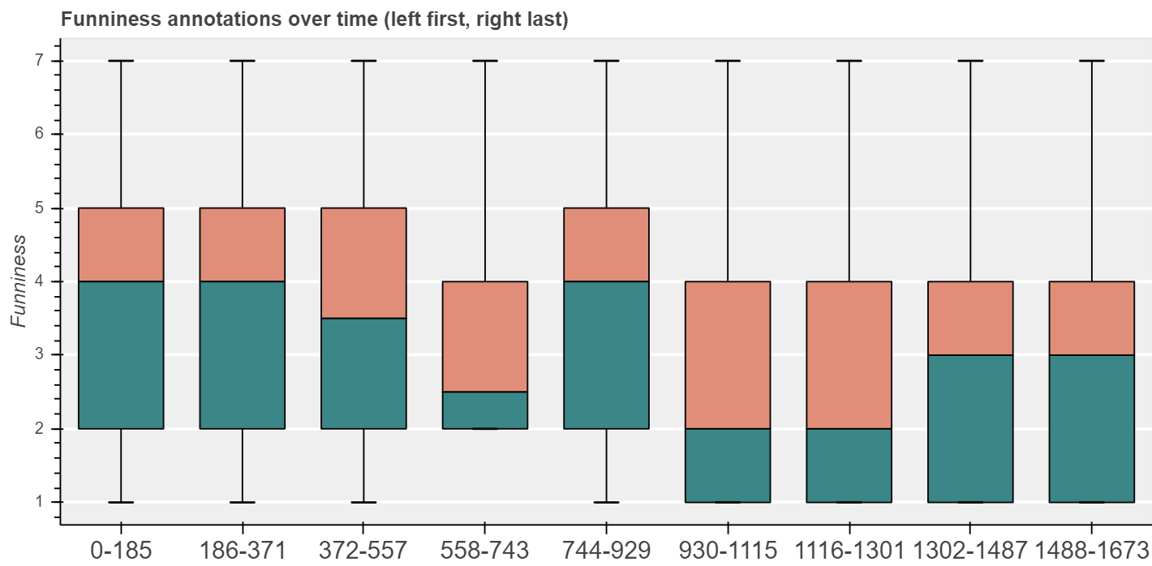
\includegraphics[width=1.0\textwidth]{graphics/average_funniness_over_time}
	\caption{Box plots of the average funniness over time in the training split.}
	\label{fig:boxplottime}
\end{figure}

A word count analysis showed that there are significant difference in the frequency of certain words. These words seem to contain certain connections to a cartoon theme. For example one of the most frequent words for funniness class 7 is "Thag" which is a common name for cartoons set in the stone age. A similar phenomena could also be observed for word phrases. For example the phrase "thousand more year" is also primarily associated with cartoons set in the stone age. A model could learn this preferences and use it to predict the funniness of a cartoon. For detailed plots please refer to figure [\ref{fig:wordocc1}], [\ref{fig:wordocc2}], [\ref{fig:phraseocc1}] and [\ref{fig:phraseocc2}].

\begin{figure}
\centering

\begin{subfigure}[b]{0.45\textwidth}
\centering
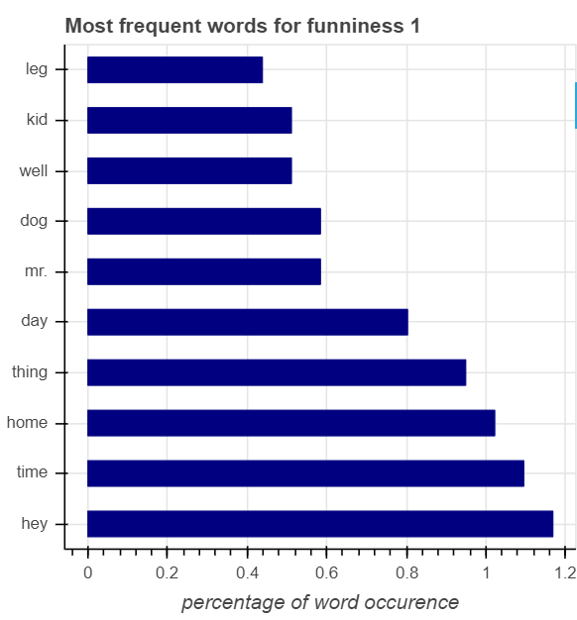
\includegraphics[width=1.0\textwidth]{graphics/word_occurence/funniness_1}
\end{subfigure}\quad
\begin{subfigure}[b]{0.45\textwidth}
\centering
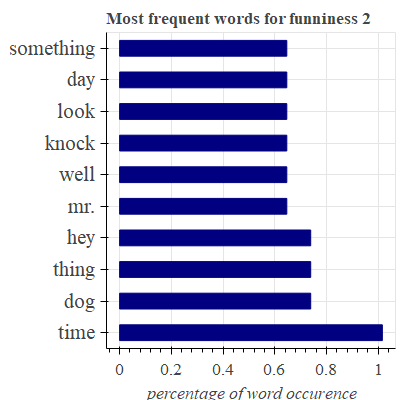
\includegraphics[width=1.0\textwidth]{graphics/word_occurence/funniness_2}
\end{subfigure}

\begin{subfigure}[b]{0.45\textwidth}
\centering
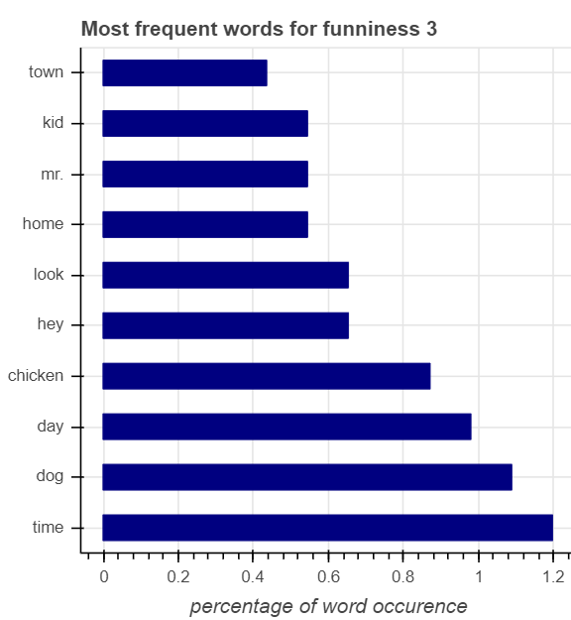
\includegraphics[width=1.0\textwidth]{graphics/word_occurence/funniness_3}
\end{subfigure}\quad
\begin{subfigure}[b]{0.45\textwidth}
\centering
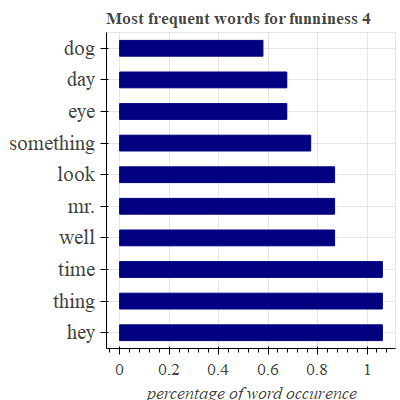
\includegraphics[width=1.0\textwidth]{graphics/word_occurence/funniness_4}
\end{subfigure}


\caption{Most frequent nouns per class 1, 2, 3 and 4.}
\label{fig:wordocc1}

\end{figure}

\begin{figure}
\centering

\begin{subfigure}[b]{0.45\textwidth}
\centering
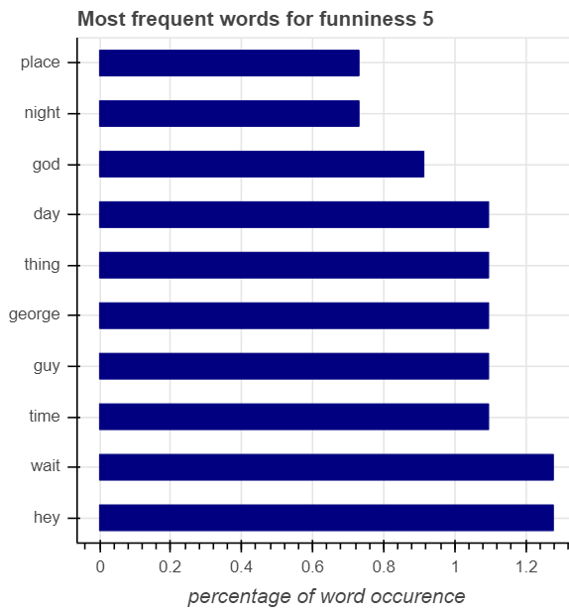
\includegraphics[width=1.0\textwidth]{graphics/word_occurence/funniness_5}
\end{subfigure}\quad
\begin{subfigure}[b]{0.45\textwidth}
\centering
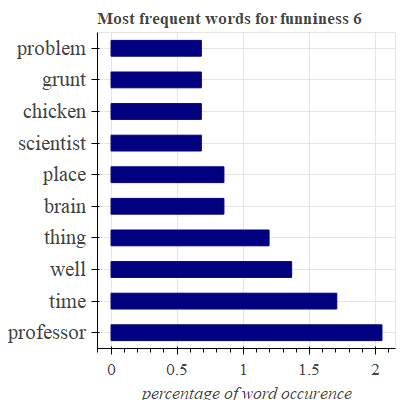
\includegraphics[width=1.0\textwidth]{graphics/word_occurence/funniness_6}
\end{subfigure}


\begin{subfigure}[b]{0.45\textwidth}
\centering
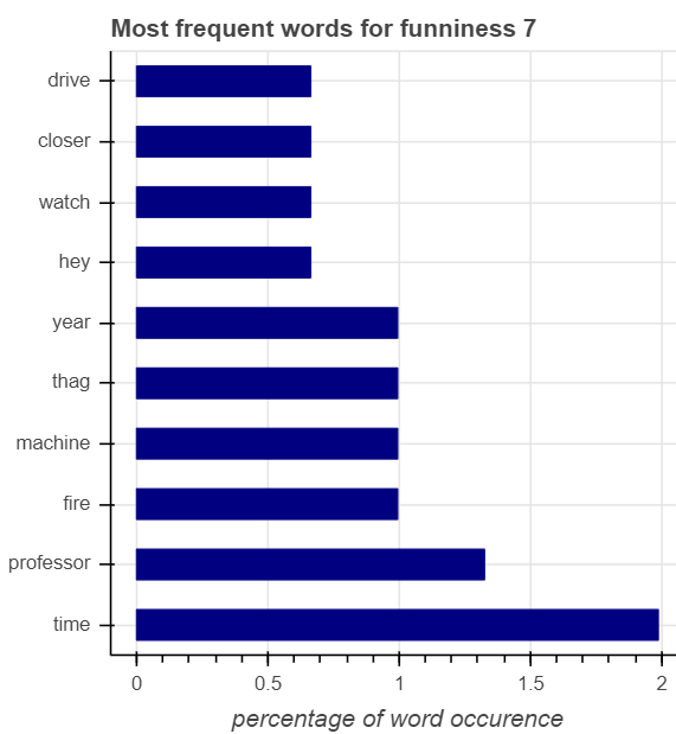
\includegraphics[width=1.0\textwidth]{graphics/word_occurence/funniness_7}
\end{subfigure}

\caption{Most frequent nouns per class 5, 6 and 7.}
\label{fig:wordocc2}

\end{figure}

\begin{figure}
\centering

\begin{subfigure}[b]{0.45\textwidth}
\centering
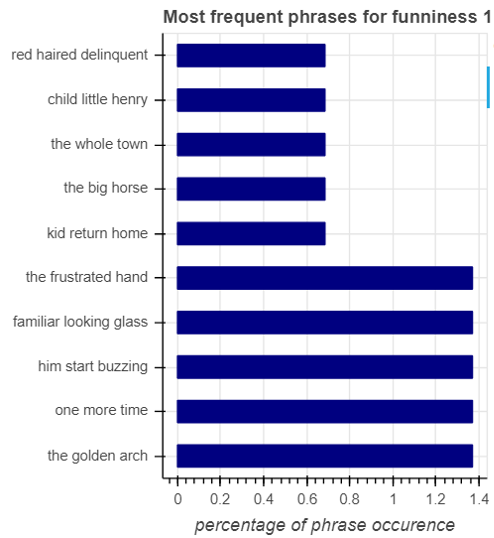
\includegraphics[width=1.0\textwidth]{graphics/phrases/funniness_1}
\end{subfigure}\quad
\begin{subfigure}[b]{0.45\textwidth}
\centering
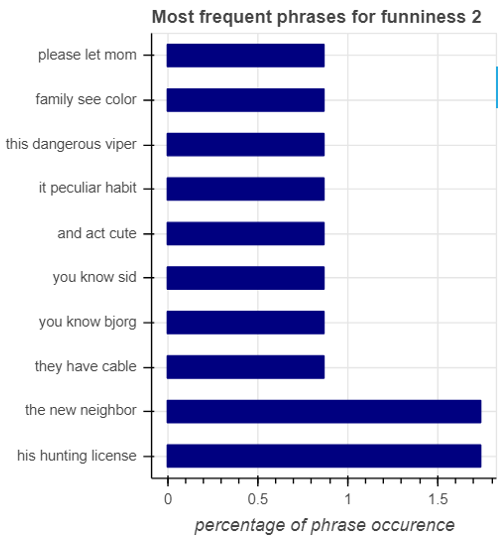
\includegraphics[width=1.0\textwidth]{graphics/phrases/funniness_2}
\end{subfigure}

\begin{subfigure}[b]{0.45\textwidth}
\centering
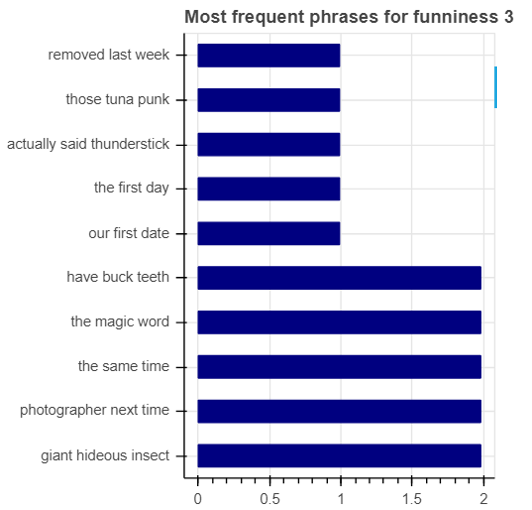
\includegraphics[width=1.0\textwidth]{graphics/phrases/funniness_3}
\end{subfigure}\quad
\begin{subfigure}[b]{0.45\textwidth}
\centering
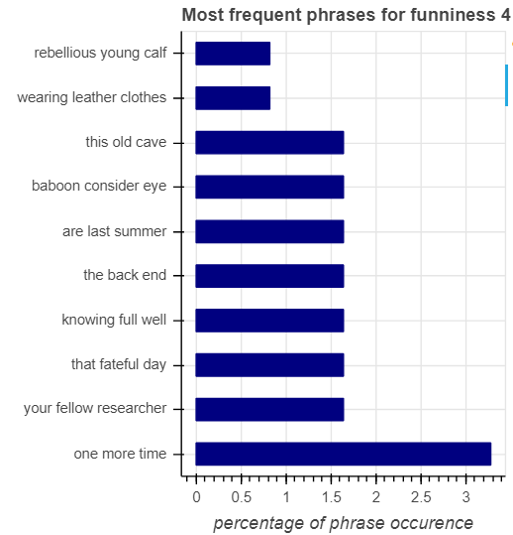
\includegraphics[width=1.0\textwidth]{graphics/phrases/funniness_4}
\end{subfigure}


\caption{Most frequent phrases per class 1, 2, 3 and 4.}
\label{fig:phraseocc1}

\end{figure}

\begin{figure}
\centering

\begin{subfigure}[b]{0.45\textwidth}
\centering
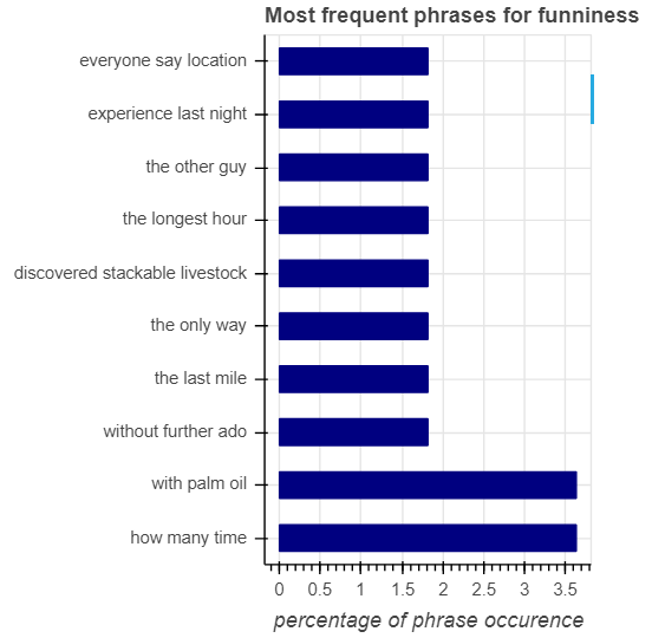
\includegraphics[width=1.0\textwidth]{graphics/phrases/funniness_5}
\end{subfigure}\quad
\begin{subfigure}[b]{0.45\textwidth}
\centering
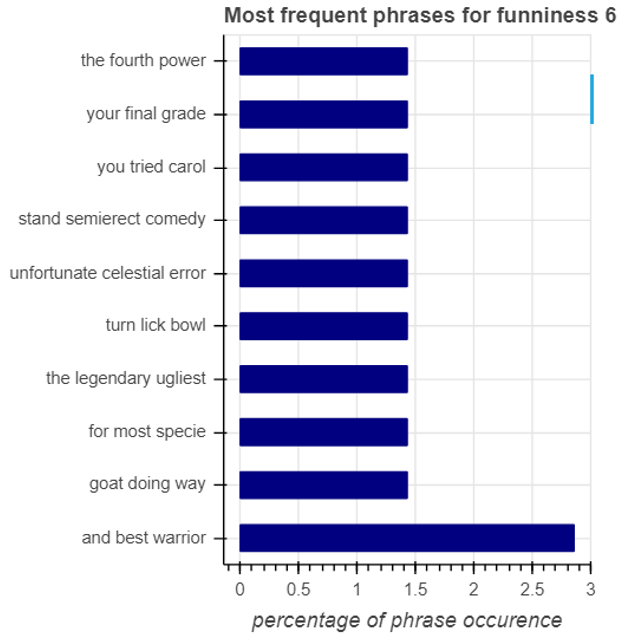
\includegraphics[width=1.0\textwidth]{graphics/phrases/funniness_6}
\end{subfigure}


\begin{subfigure}[b]{0.45\textwidth}
\centering
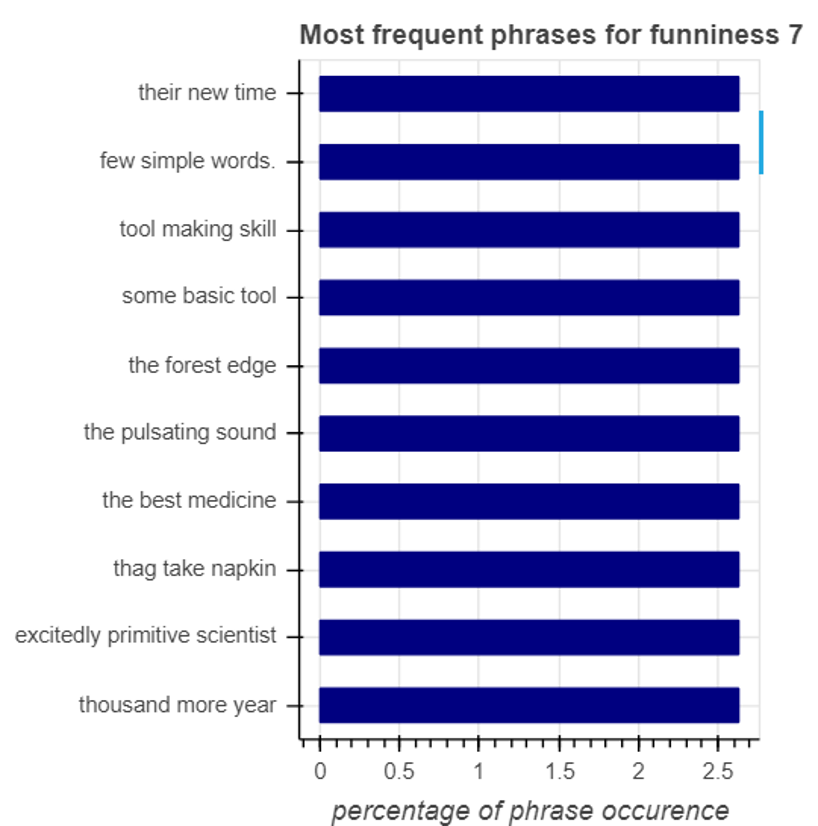
\includegraphics[width=1.0\textwidth]{graphics/phrases/funniness_7}
\end{subfigure}

\caption{Most frequent phrases per class 5, 6 and 7.}
\label{fig:phraseocc2}

\end{figure}

\section{Visual domain model design}

To reduce the problem space I decided to first tackle the visual domain of Gary Larson's cartoons. This has the advantage that there are well defined neural network architectures (CNNs, ResNet) which knowingly perform well on various image related tasks.

\subsection{Simple CNN}

The goal of this approach was to establish a performance baseline. This models goal was to answer the question: How well does a relatively simple convolutional neural network on the Gary Larson cartoon dataset?

Am important design decision a machine learning practitioner has to make is the input data format and layout. For images the number of input channels and the dimensions of the image is most relevant. Because the cartoons are grayscale the number of channels can be set to 1 without any loss of information. The input size is more difficult to set: If the input size is too large, the neural network has too much information to process and cannot find discriminative patterns. A comparison would be to play the game "Where is Waldo" on an image of the size of a football field. On such image, it would be for humans also very difficult to find the right pattern (in this case Waldo).

Otherwise, if the input size is too small, then crucial information may get lost as well. Resizing an image can be seen as a crude form of dimensionality reduction, as the dimensionality of the data is reduced. Another important consideration is, that 90\% of the images are in lanscape, while the remaining are in portrait orientation. Therefore, predicting the image in lanscape well has priority.

Different configurations for the input size was empirically probed and validated using the validation set. This includes the average size of cartoons, average size of landscape cartoons, several downscaled image sizes. The final best input size was 141x174.

Modelling the output of a neural network is equally crucial as the input. I performed two experiments: One where the network was modelled in a classification setting where the final neurons returned a one hot encoding of the funniness. for classification I used cross entropy loss. Another experiment was modelled as a  regression task, where the final neuron returned the funniness directly. I tested both L1 loss (mean absolute error) and L2 loss (mean squared error) for regression. The regression neural networks did not even approximate the baselines on the validation set, which is the reason why I did not pursue this approach any further.

Another important hyperparameter of CNNs is the number of layers and number of neurons per layer. As the dataset is relatively small in deep learning terms, it was not possible to train too many layers, while too less layers would mean that the network does not have enough capacity to learn the necessary concepts of humor. The final network consists of two convolutional blocks and one fully connected dense layer at the end. Their depth is set to 100.

\todo {Illustration des CNN Netzwerks}

\if false
Seiten: 1

\begin{itemize}
\item Wie wurde die größe des Input Layers definiert: Verschiedene Kombinationen probiert. Skalierung mit Aspektratio der Cartoons. 
\item Visuelle Illustration des finalen Netzwerks
\item Einmal als Regressionstask und einmal als Klassifikationstask modelliert => Klassifikation funktionierte besser
\item Verschiedene Anzahl an Layer und Größe an Layer probiert
\end{itemize}

\fi

\subsection{Transfer Learning CNN}

As described in section \ref{transferlearning} transfer learning is a common approach to deal with a small dataset in deep learning. This experiment uses a pretrained ResNet18 model. \cite{resnet} ResNet consists of multiple residual blocks, which allows the network to be much deeper compared to a naive CNN and still improve performance. Earlier blocks perform simple feature extraction and later blocks perform high level feature extraction. 

I probed several configurations of this transfer learning approach:

\begin{enumerate}
\item Reuse entire convolutional feature extractor and retrain final classifier
\item Retrain last block of ResNet18 and the final classifier
\item Reuse entire model and add a new final fully connected dense layer
\end{enumerate}

The second approach was the best performing on the validation set. Additionally applying data augmentation was crucial. The following transformations on the cartoon image were most successful:

\begin{itemize}
\item Random horizontal flip
\item Random resize and crop
\item Random rotation
\end{itemize}

\todo {Illustration vom transfer learning}

\if false
Seiten: 1

\begin{itemize}
\item Architektur (ResNet18) verwendet und auf Cartoons angewandt
\item Welche Parameter wurden transferiert? Einmal wurde kompletter Convolutional Teil transferiert, einmal wurde letzter Block auch trainierbar geschaltet und einmal wurde der fully connected teil ebenfalls übernommen.
\item Data Augmentation
\item Visuelle Illustration des gewählten besten Netzwerks

\end{itemize}
\fi


\subsection{Transfer Learned Object Detection}

\begin{figure}[ht]
	\centering
  	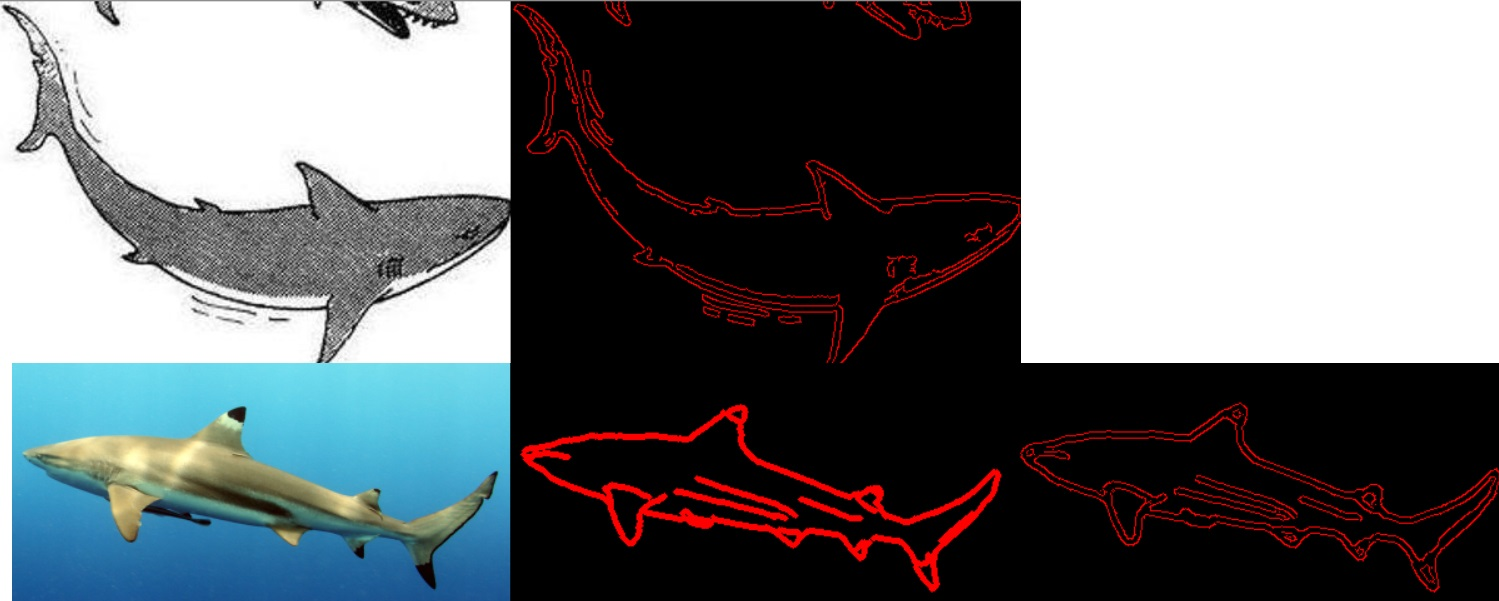
\includegraphics[width=1.0\textwidth]{graphics/edge_edge_detection.jpg}
	\caption{First row is a shark drawn by Gary Larson. Second row is a real world shark.}
	\label{fig:dataugmentation}
\end{figure}

There were two suspected issues with the previous transfer learning approaches:

\begin{enumerate}
\item The source domain was too distinct from the target domain. The domain of real world images (which ResNet18 was trained on) and cartoons is too distinct for a naive transfer learning approach. I addressed this issue by implementing a novel data augmentation technique.
\item The semantic level of humor may be too high for CNNs to understand. I planned to adress this issue by extracting high-level feature vector based on object detection using CNNs.
\end{enumerate}

The data augmentation (1) illustrated in figure \ref{fig:dataugmentation} works by applying the canny edge detection filter multiple times. The cartoon image is transformed by Canny (using default parameters) into a target domain. The real world image is transformed by applying Canny twice. The first application has a stroke size similar to the average size of Gary Larson strokes. The second application of Canny with the same parameters should bring the real world images into the same target domain.

\begin{table}[]
\label{objectdetectionfeaturevector}
\centering
\begin{tabular}{|l|l|l|l|l|l|}
\hline
Has Human? & Has Dogs? & Has Cats? & Has Alien? & Has Shark? & ... \\ \hline
1   & 1 & 1 & 0 & 0 & ... \\
\hline
\end{tabular}
\caption{Hypothetical feature vector}
\end{table}

To improve the problem of high-level semantics (2) I wanted to train an object detection model based on the CIFAR-100 dataset augmented using the double edge detection data augmentation.\cite{cifar100}This would allow to compute a high-level description of a cartoon based on the objects detected by the object detection algorithm. To validate this approach I first trained a simpler image classification model based on ResNet18. If image classification does not sufficiently work, then object detection will most likely also fail. As an example the feature vector of the figure \ref{fig:fig1} could look similar to \ref{objectdetectionfeaturevector}.

Unfortunately this approach did not achieve significant results, as there were no consistent classifications. Therefore I did not train the final object detection. If, for example, a person was consistently assigned the same class, then the feature vector could have entailed enough semantic information for cartoon theme-based predictions. The data analysis revealed that there are certain cartoon themes which have higher funniness scores compared to others. 

Another approach I tried was to train an object detection model based on other datasets: The TU Berlin sketch dataset and Googles Quick, draw! dataset.\cite{tuberlin}\cite{quickdraw} Theses approaches did not need the edge detection preprocessing, as they were already in the sketch domain. Still the domains were too distinct, as the image classification performance never reached significant performance.

\if false

Seiten: 1.5

\begin{itemize}
\item Initiale Idee erklären: Cartoons durch Feature Vektor der vorhandenen Objekte erklären
\item Beispiel eines solchen Featurevektors bringen
\item Zuerst soll Image Classification der einzelnen Objekte funktionieren
\item Woher bekommt man ein solches Datenset? Idee: Existierendes Cifar100 (datenset mit 100 bildkategorien) durch image preprocessing (doppelte kantenerkennung) in selbe Bilddomain bringen und dort trainieren
\item Beim Anwenden des Datensets (1x Kantenerkennung auf Gary Larsons Cartoons) extrem schlechte Performance: Keine Muster erkennbar
\item Dadurch lassen sich die Cartoons nicht als featurevektor repräsentieren
\item Ueber 100 Objekte von Gary Larsons Cartoons wurden dafür extra annotiert => Keine Muster erkennbar
\item Graphische Darstellung wie Objekte in selber Domäne hätten sein können (Hai Bild)
\item Evtl. verbesserungsmöglichkeiten erklaeren.
\item Evtl. dass das image classification am data augmented cifar100 auch eher schlecht funktioneirte
\end{itemize}

\fi

\section{Text domain model design}

Erläutern wie danach nur die Text Domain berücksichtigt wurde.

Seiten: 0.25

\subsection{ELMo}

First I tried to model the punchlines using an LSTM neural network architecture. This approach quickly overfitted. GRU cells had the same problem. I probed several architectures with multiple LSTM cells, different hyperparameters and an additional embedding layer.

Recurrent neural networks require big datasets, the idea then was to train simpler models. I achieved this by generating a sentence embedding from the sequence of word embeddings. A sentence embedding is a vector representation of a word embedding in a vector space. There are many different ways to obtain such embedding. I chose the simple approach to take the mean of all word embeddings of a punchline. This resulted in a fixed sized vector representation of a punchline, which allowed the use of a regular fully connected neural network.

I chose ELMo as the main context-aware word embedding for this thesis. \cite{elmo} Mainly due to the state-of-the-art results it achieves while still being relatively easy to use in the chosen NLP framework. More about this in chapter \ref{implementationchapter} Implementation.

\todo{Illustration des Netzwerks}

\if false

Seiten: 1.0

\begin{itemize}
\item Gewählte ELMo Ansätze erklären
\item Zuerst wurde LSTM/GRU probiert. Problem: Overfitting
\item Danach wurde simpler Classifier mit Sentence Embedding angewandt (Sentence Embedding ist ein Vektor für den gesamten Satz statt pro Wort)
\item Visuelle Illustration des gewählten Netzwerks

Das eher bei Design:
\item ELMo vs BERT: Warum wurde ELMo verwendet. Grund: Einfache Verwendung mit gewähltem Framework AllenNLP und performance war vergleichbar bei vielen NLP Tasks
\end{itemize}
\fi

\subsection{AutoML}

Seiten: 1

\begin{itemize}
\item AutoML Ansatz erklären
\item Wieso angewandt? Vielleicht findet Computer Hyperparameter besser
\item Vielleicht funktioniert zB eine SVM besser für gewählten Task
\item Wie wurde Feature Vektor erstellt? => TFIDF, GloVe, ELMo, TFIDF + GloVe, TFIDF + ELMo
\end{itemize}

\section{Visual and text domain combined model design}

Erläutern wie danach beide Domänen zusammen berücksichtgt wurden.

\subsection{Two Stage Model}

Seiten: 2

\begin{itemize}

\item Probleme der vorigen Ansätze erläutern: Fokus wurde zu sehr auf die häufigsten Klassen gelegt. Die seltenen Funniness Klassen wurden nie vorhergesagt
\item Lösung: Für jede Funniness Stufe ein eigenes model trainieren und ein finales Model nehmen, welches basierend auf den vorigen Stufen die finale Prediction durchführt
\item 1 vs Rest Classifier erklären
\item Finale Regression erklären.
\item Modulares System erlaubte auch einfaches Kombinieren von text und Bild
\item Oversampling wurde ebenfalls verwendet
\item Autoencoder wurde auch verwendet (Cartoon Bilder dimension reduzieren)
\item Visuelle Illustration erklären
\item Klassengewichtung in 1 vs Rest Classifier

\end{itemize}

\if false
\section{Additional Experiments}
A list of experiments performed but did not make the cut for a more detailed analysis:

\begin{itemize}
\item \textbf{LSTM / GRU}: Overfitting was a big problem early on
\item \textbf{Wasserstein Loss instead of Cross Entropy Loss}: Idea was to penalize near misses less.
\item \textbf{L1 Loss}: Model as a regression task. Model was not even able to approximate the Average Baseline using this approach
\item \textbf{Applying a discrete cosine transformation (DCT)}: Since convolutions are not well suited for line drawings the idea was to apply a DCT beforehand. 
\item \textbf{Advanced Two Stage Model}: Add different binary classifiers in the first stage.
\item \textbf{Loss Weighting of Two Stage Model}: Try different penalties for different kind of errors in the first stage. For example add more penalty for true positives compared to false negatives.
\item \textbf{Preprocessing of cartoons}: Apply different filters on cartoons. For example: Canny edge detection.
\item \textbf{Word vector combinations}: Many different word vector combinations of TFIDF, GloVe and ELMo. 
\end{itemize}

Hier muessen eventuell Sachen rausgenommen werden die doch erwaehnt wurden bzw. worden sind.
\fi

\chapter{Implementation} \label{implementationchapter}

Erläuterung des Implementierungsvorgangs

Seiten: 0.25

\section{Technical Foundation}

Seiten: 2

\begin{itemize}

\item Wahl der Library und Frameworks erläutern: PyTorch, pandas, sklearn, Python, AllenNLP
\item Entwicklungsumgebung und Reproduzierbarkeit (git, Fixierter Random Seed, deterministischer Modus von PyTorch)
\item Gewähltes Command Line Interface: Relevante Parameter via CLI steuerbar machen
\item Warum wurde gegen Jupyter Notebooks entschieden? Reproduzierbarkeit und weitere Gründe

\end{itemize}

\section{Annotation Tool}

Seiten: 1

\begin{itemize}
\item Wieso wurde eine Annotierungsapplikation implementiert?
\item Hat es sich gelohnt? Wie lange Zeit wurde durchschnittlich pro Annotierung gebraucht vs. wie lange hätte es mit Excel gedauert? Entwicklungsdauer des Annotierungstool?
\item Technik vom Annotierungstool (Python, Django)
\item Bild vom Annotierungstool
\end{itemize}


\section{Debugging of models}

Seiten: 1.5

\begin{itemize}
\item Wie wurde sichergestellt dass Netzwerke funktionierten? 
\item Einerseits indem die Outputs überprüft wurden (kommt NaN raus oder nur 0?)
\item Cartoon Bilder und Text wurde durch Bilder ersetzt die die entsprechende Klasse des ursprünglichen Cartoons enthielten => Sofort sehr gute Werte
\item Problem war auch, dass einmal der Training/Test/Validation Split fehlerhaft war und deswegen anfangs die Werte viel zu gut waren => Sei immer skeptisch deinen Resultaten gegenüber.
\end{itemize}


\section{Detailed Architecture}

Seiten: 2

\begin{itemize}

\item Detailliertes Klassendiagramm für das Datenmanagement und Erklärung
\item Detailliertes Klassendiagram für das Evaluationssystem und Erklärung
\item Detailliertes Klassendiagramm für das Experimentsystem und erklärung 
\item AutoML Architektur erwähnen
\item AllenNLP Architektur erklären
\item Conclusio: Overengineering vermeiden, da Code Wiederverwendung sehr schwer ist. Ursprünglich war geplant die Architektur für des Convolutional Teils für den TExt Teil wieder zu verwenden. Letztendlich war es einfacher stattdessen AllenNLP zu verwenden

\end{itemize}


\chapter{Evaluation}

This chapter aims to evaluate the performance of the implemented architectures. In
general the results show that this problem is very hard. Despite the progress in the field of Deep Learning it was not possible to beat the baseline. \\

The cartoon dataset is split into three sub sets:

\begin{itemize}
\item Training Set: 1492 samples (70\%)
\item Validation Data: 746 samples (20\%)
\item Test Data: 249 samples (10\%)
\end{itemize}

The experiments were run on a PC running Ubuntu 18.04 LTS using PyTorch 1.0 and
Python 3.6. The hardware is a GTX 1070 Max-Q with an Intel Core i7-8750H. For more
information regarding the build set up and necessary environment please refer to the GitHub Repository \cite{deephumorrepo}.

The hyperparameters were chosen based on best practice and previous
experience by the author with deep neural network training. Because there are many hyperparameters an automated search of the hyperparameter space is infeasible with the hardware available to the author.

\section{Architectures}
Several architectures have been implemented and are evaluated in the following sections.


\subsection{Baseline}

Four baseline strategies have been selected: 

\begin{itemize}

\item Most Frequent Baseline: Picks the most frequent label in the dataset.
\item Average Baseline: Returns the average funniness of the dataset. For the accuracy metric the average is rounded using round to nearest integer.
\item Random Baseline: Returns a random funniness picked uniformly from one to seven.
\item Stratified Baseline: Returns a funniness sampled from the distribution of the
training set.

\end{itemize}

For the mean absolute error metric the average performed best, while for the accuracy score the most frequent class has the best score.

\subsection{Simple CNN}
The simple CNN architecture overfits very quickly. The accuracy and MAE scores are very similar to the most frequent baseline, which indicates that the model most likely learns to return the most frequent class.

\subsection{Transfer Learning of Pretrained ResNet18}
Noteworthy about this approach is that also enabling the data augmentation in the testing/validation phase makes this approach better than the baseline. The exact reason is not obvious, but indicates that the model expects the cartoons to be augmented.

The data augmented version of this experiment unexpectedly achieved the best results during testing phase.

Sampling for each class a cartoon and examining the output layer of the trained neural network reveals some interesting insight about how the model works. In general the results show, that the classifier never assigns high confidence into the predictions. No classification assigns a probability higher than 40\%.

When examining the distribution across the different predictions over the different samples it seems that the general distribution does not change significantly. Some deviations are present, for example when comparing the probabilities for funniness 2.

In general it seems that the model often ignores the input data and instead learns the label distribution. The similarities between the predictions and the histogram of funniness occurrences are very high. Compare figure [\ref{fig:figdistr1}] and figure [\ref{fig:figdistr2}] with figure [\ref{fig:labeldistr}].

\begin{figure}
\centering

\begin{subfigure}[b]{0.45\textwidth}
\centering
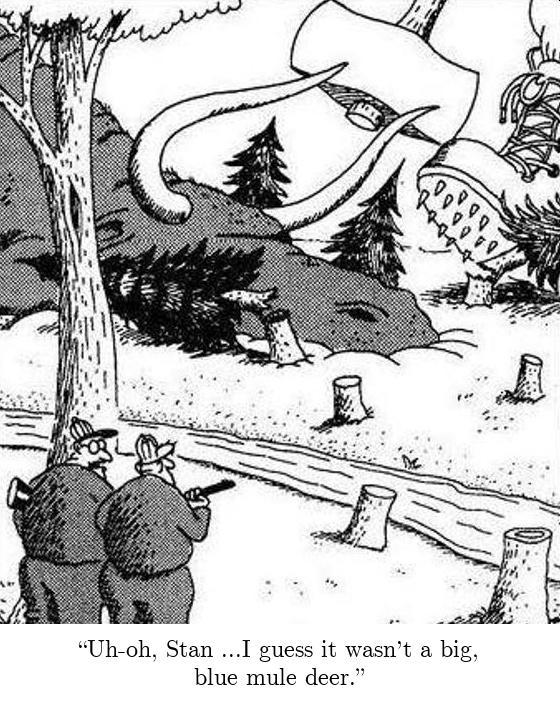
\includegraphics[width=0.9\textwidth,height=0.3\textheight,keepaspectratio]{graphics/detail/Test_for_Image_1_cartoon} \\
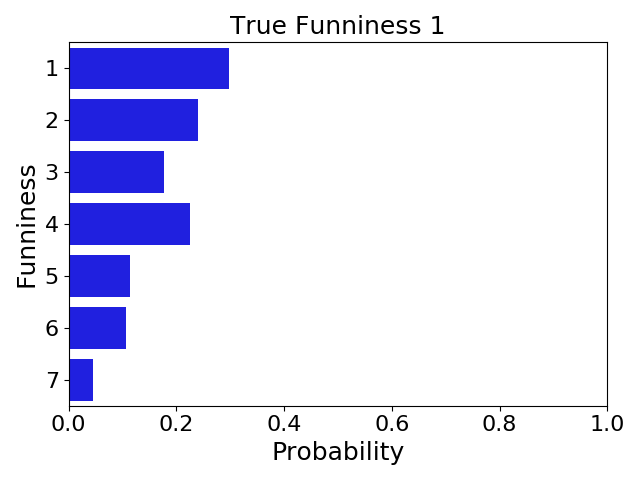
\includegraphics[width=1.0\textwidth]{graphics/detail/Test_for_Image_1}
\end{subfigure}\quad
\begin{subfigure}[b]{0.45\textwidth}
\centering
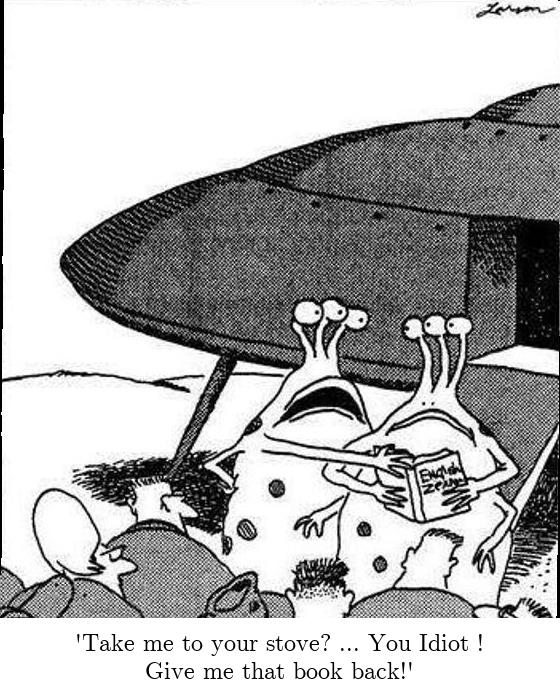
\includegraphics[width=0.9\textwidth,height=0.3\textheight,keepaspectratio]{graphics/detail/Test_for_Image_2_cartoon} \\
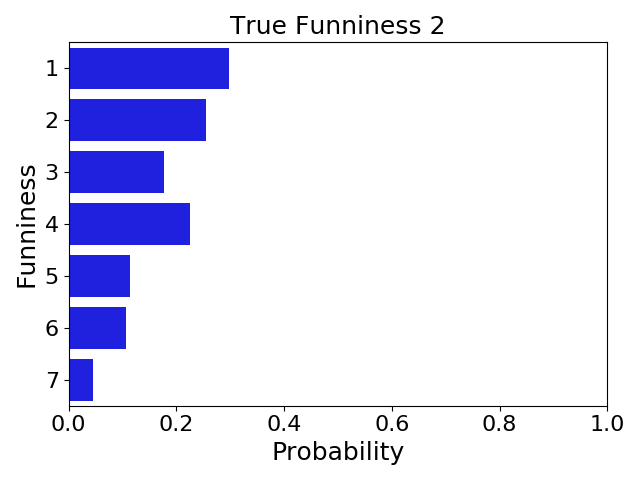
\includegraphics[width=1.0\textwidth]{graphics/detail/Test_for_Image_2}
\end{subfigure}

\begin{subfigure}[b]{0.45\textwidth}
\centering
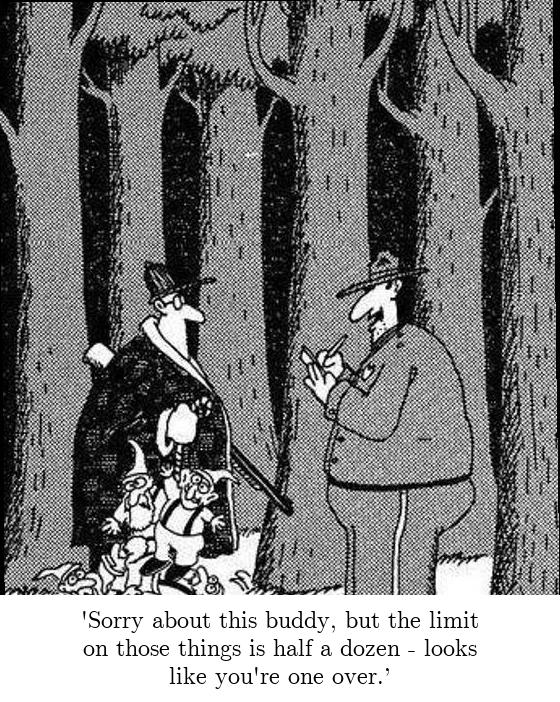
\includegraphics[width=0.9\textwidth,height=0.3\textheight,keepaspectratio]{graphics/detail/Test_for_Image_3_cartoon} \\
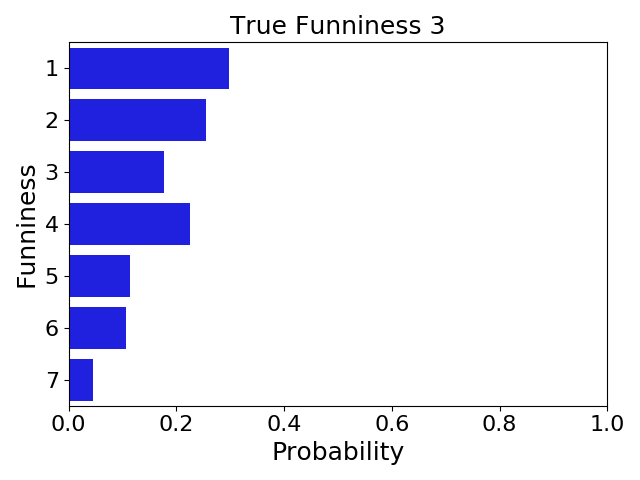
\includegraphics[width=1.0\textwidth]{graphics/detail/Test_for_Image_3}
\end{subfigure}\quad
\begin{subfigure}[b]{0.45\textwidth}
\centering
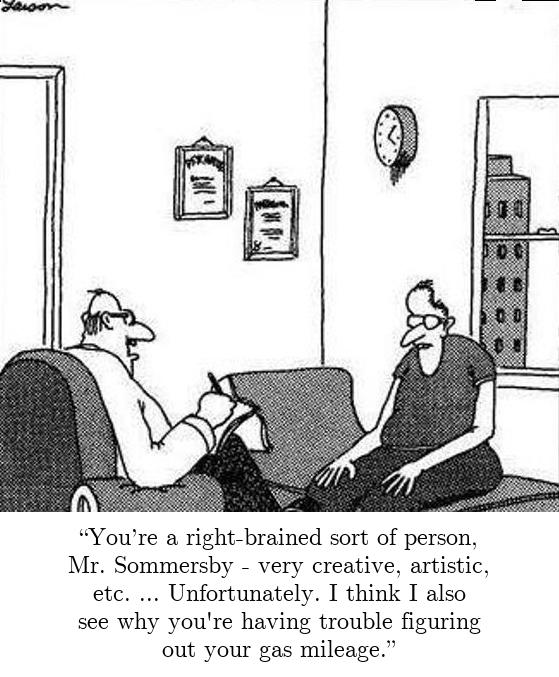
\includegraphics[width=0.9\textwidth,height=0.3\textheight,keepaspectratio]{graphics/detail/Test_for_Image_4_cartoon} \\
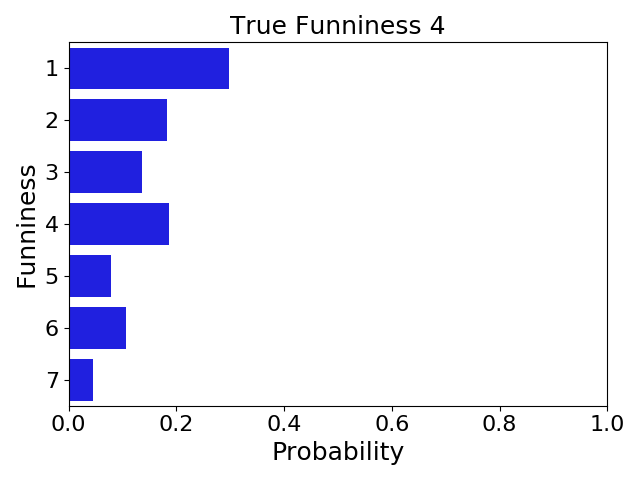
\includegraphics[width=1.0\textwidth]{graphics/detail/Test_for_Image_4}
\end{subfigure}

\caption{For the classes 1, 2, 3 and 4: The bar plots represent the probability the classifier assigned each category for the cartoon above.}

\label{fig:figdistr1}

\end{figure}


\begin{figure}
\centering

\begin{subfigure}[b]{0.45\textwidth}
\centering
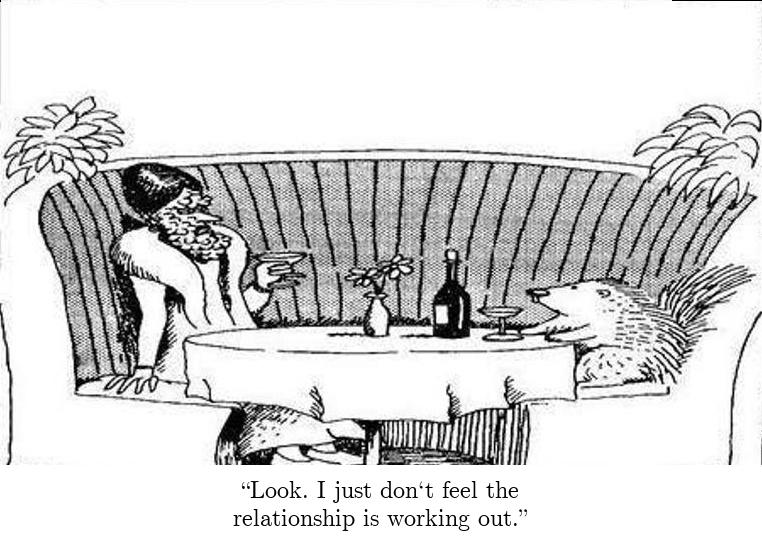
\includegraphics[width=0.9\textwidth,height=0.3\textheight,keepaspectratio]{graphics/detail/Test_for_Image_5_cartoon} \\
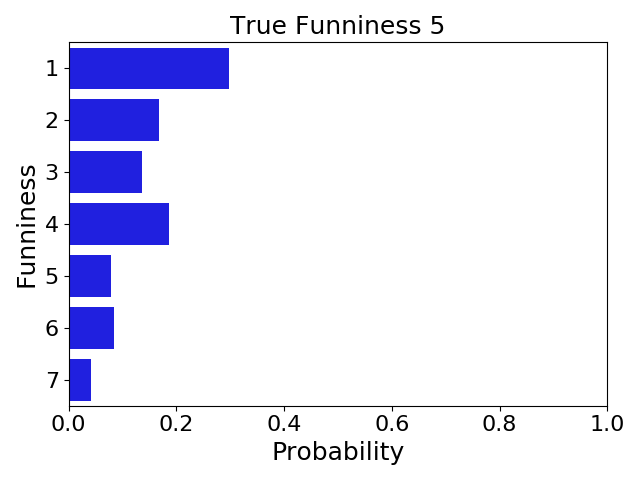
\includegraphics[width=1.0\textwidth]{graphics/detail/Test_for_Image_5}
\end{subfigure}\quad
\begin{subfigure}[b]{0.45\textwidth}
\centering
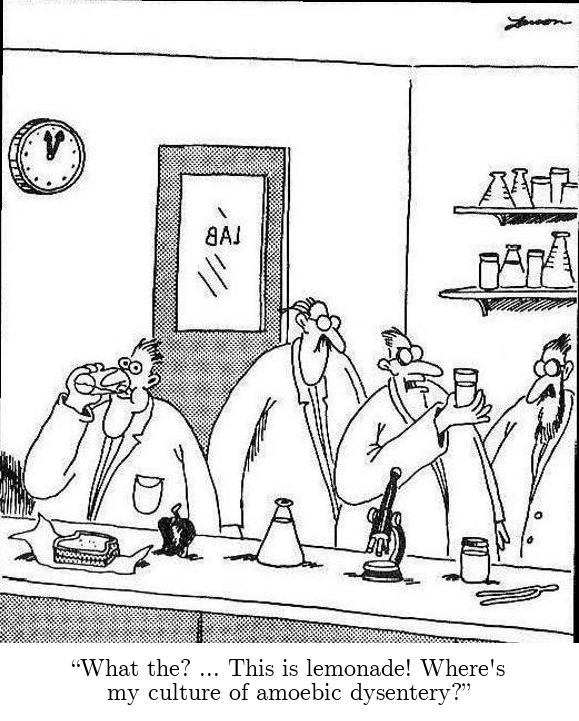
\includegraphics[width=0.9\textwidth,height=0.3\textheight,keepaspectratio]{graphics/detail/Test_for_Image_6_cartoon} \\
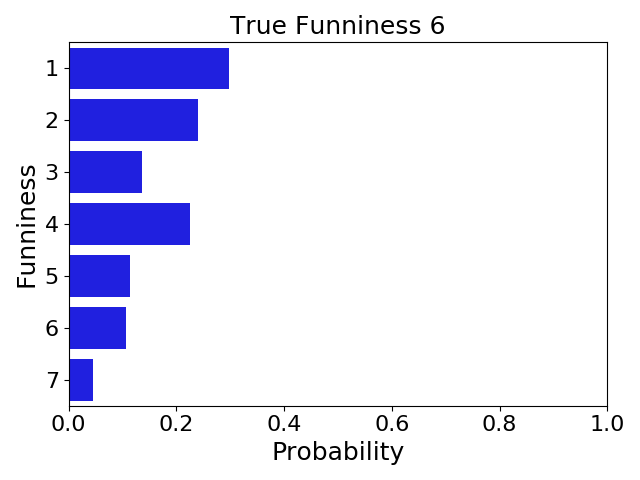
\includegraphics[width=1.0\textwidth]{graphics/detail/Test_for_Image_6}
\end{subfigure}

\begin{subfigure}[b]{0.45\textwidth}
\centering
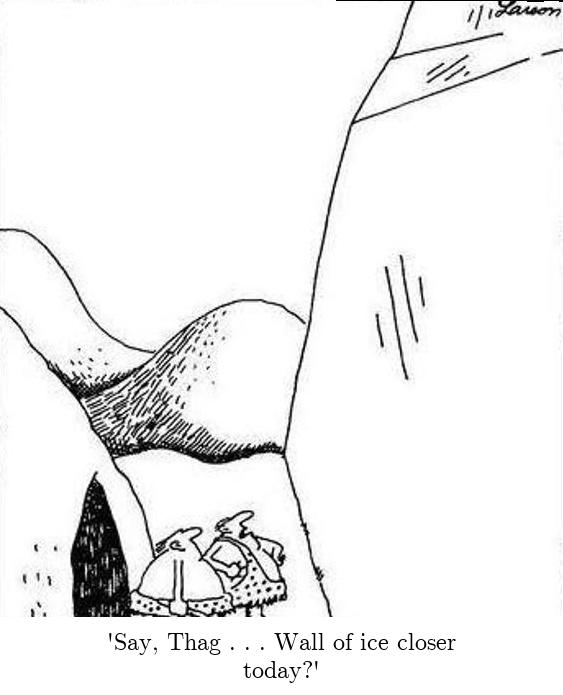
\includegraphics[width=0.9\textwidth,height=0.3\textheight,keepaspectratio]{graphics/detail/Test_for_Image_7_cartoon} \\
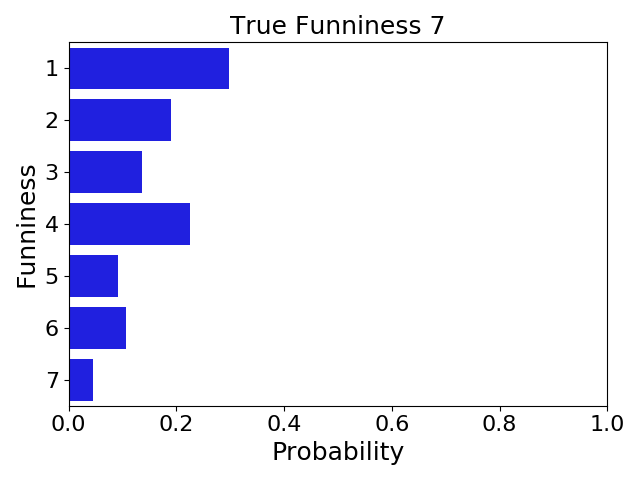
\includegraphics[width=1.0\textwidth]{graphics/detail/Test_for_Image_7}
\end{subfigure}\quad
\caption{Continued for the classes 5, 6 and 7.}
\label{fig:figdistr2}

\end{figure}

\begin{figure}
	\centering
  	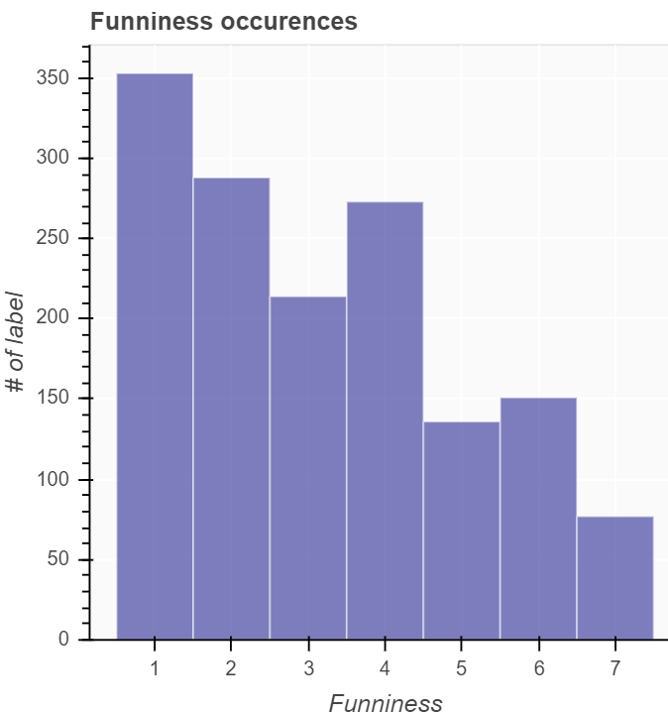
\includegraphics[width=0.75\textwidth]{graphics/label_distribution.png}
	\caption{The label distribution of the training set}
	\label{fig:labeldistr}
\end{figure}

\subsubsection{Confusion Matrix}
\begin{figure}
	\centering
  	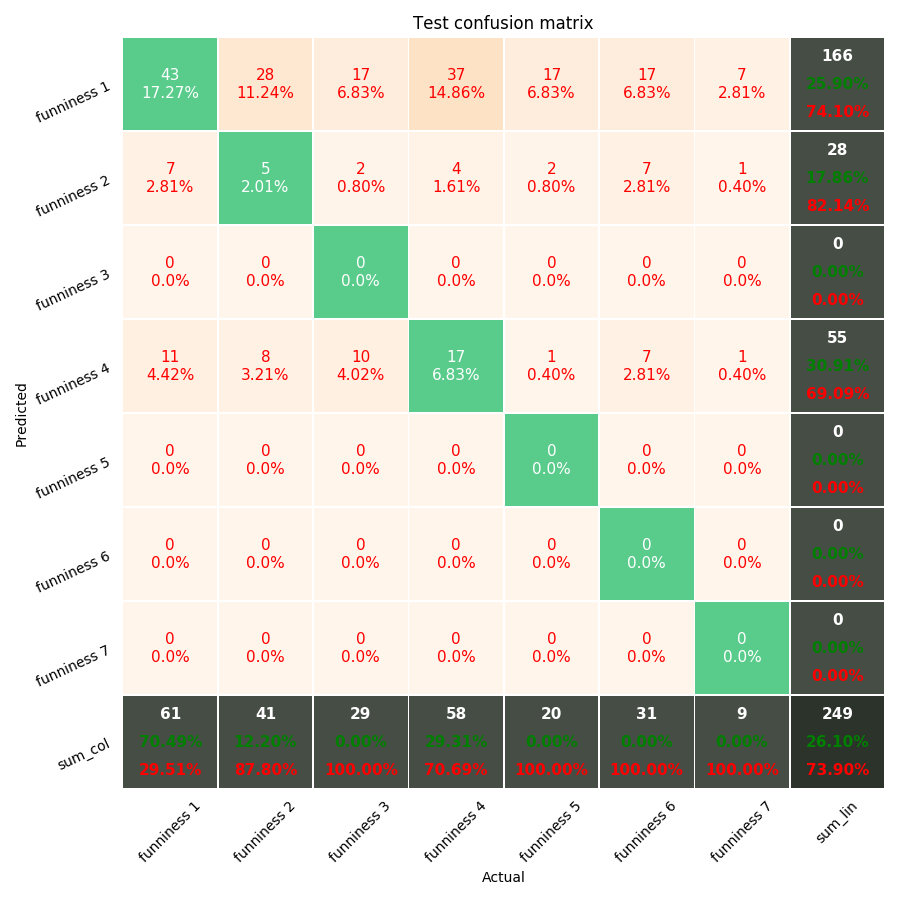
\includegraphics[width=1.0\textwidth]{graphics/transfer_confusion_test.png}
	\caption{Confusion Matrix of the transfer learning CNN (with data augmentation) on the test split}
	\label{fig:confusionmatrixtransferlearningtest}
\end{figure}

\begin{figure}
	\centering
  	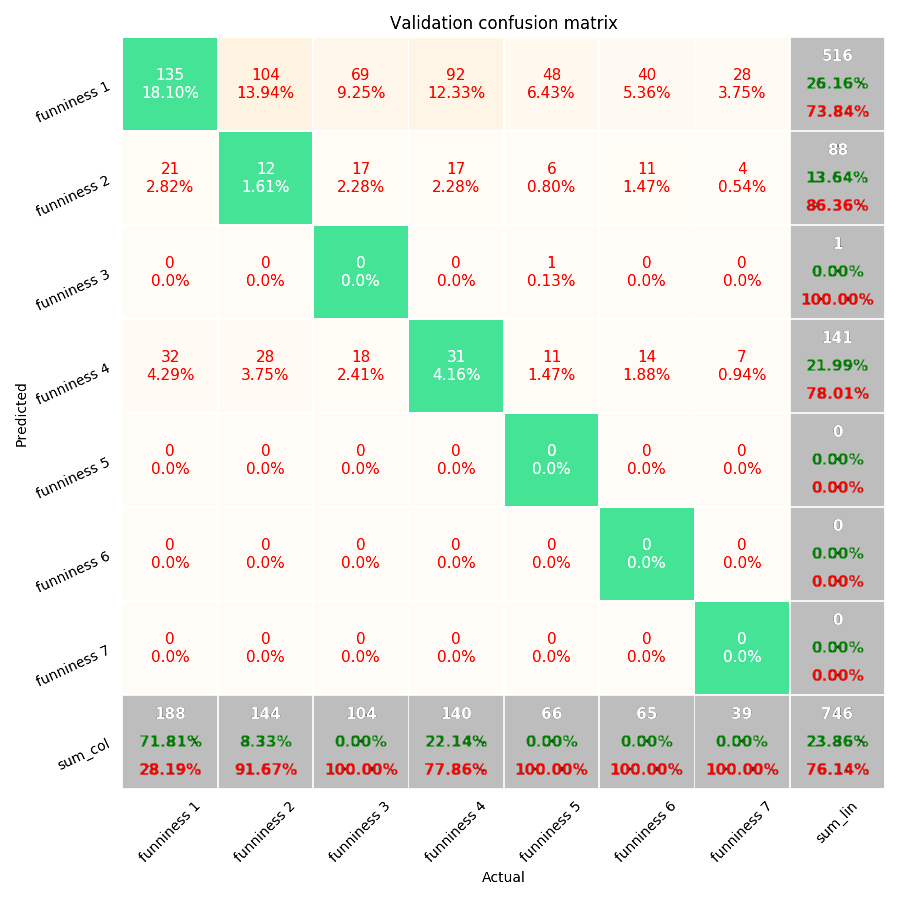
\includegraphics[width=1.0\textwidth]{graphics/transfer_confusion_val.png}
	\caption{Confusion Matrix of the transfer learning CNN (with data augmentation) on the validation split}
	\label{fig:confusionmatrixtransferlearningval}
\end{figure}

One can clearly see that for both the validation and test split the model learned to approximate the label distribution, instead of learning to generalize the underlying structure. The three most frequent funniness classes (1, 4 and 2) are the only ones the model predicts and are therefore by chance correct. Other classes are not predicted at all by the classifier. This motivated the design of the two stage model, where specific models are trained for each funniness class.


\subsection{Transfer Learned Object Detection}

The result of the object detection approach are incomparable to the other results, as it was not implemented far enough to return any labels. It was not further developed, as the predicted objects for each object were essentially random.

\subsection{ELMo Pretrained Model}

Based on the pretrained ELMo model this model initially looked the most promising, as it
achieved the highest validation accuracy. Unfortunately this was only due to overfitting,
as during test phase the performance dropped.

Most likely a problem of this approach is that many insider jokes are lost, due to the fact
that the pretrained vocabulary of the ELMo model does not contain many of them, so
they can not be used by our model. For example the word "Thag" which is one of the most frequent terms for cartoons with funniness 7 is not in the ELMo vocabulary and therefore ignored.

\subsection{AutoML Model}
Initially, when testing on the validation set, the TFIDF configuration looked very promising, as it achieved top results with a very simple feature representation. The test set
revealed overfitting. The ELMo feature representation performed worse in both settings.
Since the TFIDF feature representation would not have relied on a pre-trained vocabulary
it would not have suffered by the problem of domain specific words.

For this experiment the library hyperopt-sklearn \cite{hyperopt} was used, as it accomplishes state-of-the-art AutoML performance.

\subsection{Two Stage Model}
The Two Stage Models is not better than the average baseline. The idea of trying to avoid overfitting by using multiple classifiers for each funniness did not work as expected.

Combining the visual and text information did improve the results, but not significantly. The MAE
score is on par with the baseline, while still beating it at the accuracy score. This improvement is still very weak.
understands humor.

One problem identified was the fact, that the images contained much more data compared to the punchlines. To tackle this problem, the idea was to use a deep autoencoder. This reduces the feature size of the images significantly. But against our expectation it did not improve the results compared to previous attempts.

When comparing the MAE of the Two stage model (figure [\ref{twostagemae}]) an interesting phenomena can be observed: Even though the performance is very similar to the average baseline, the actual MAEs per class are different. This means that the model does not simply return the average funniness, but does something else.

\begin{figure}
\centering
\begin{tabular}{|l|l|l|l|l|l|l|l|} 
\hline
\textbf{Funniness} 	& \textbf{1}	& \textbf{2}	& \textbf{3}	& \textbf{4}	& \textbf{5}	& \textbf{6}	& \textbf{7}  \\ 
\hline
Two Stage Model     & 2.42			&  1.57			& 0.97			& 0.8			& 1.53			& 2.28			& 3.64   \\
Baseline Average    & 2.21			& 1.21			& 0.21			& 0.79			& 1.79			& 2.79			& 3.79 \\	
\hline
\end{tabular}
\caption{MAE per class}
\label{twostagemae}
\end{figure}

A confusion matrix of each classifier in the first stage reveals whether this approach could be effective. If all classifiers have a reasonable accuracy the second decision stage has a higher chance of predicting the correct class. If the first stage only returns noise the second stage would not be able to beat the average baseline.

It seems that the first stage is not effective in doing so. For funniness 3, 4, 5, 6 and 7 there is no true negative, which means that the model for this class only learns to always return 1.

\begin{figure}
\centering

\begin{subfigure}[b]{0.45\textwidth}
\centering
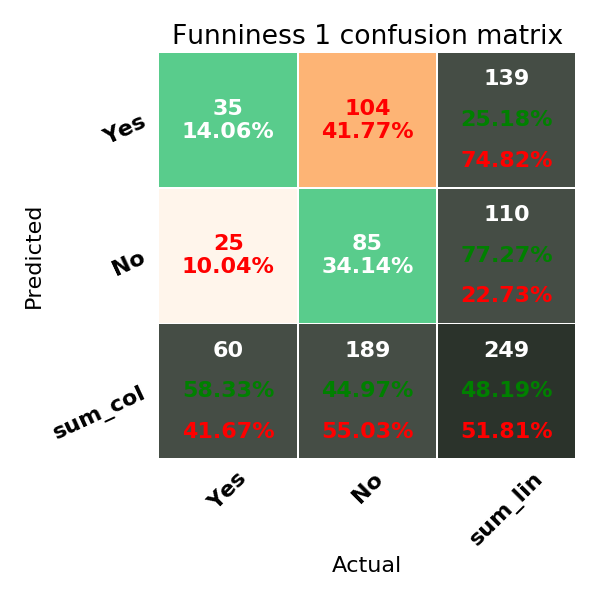
\includegraphics[width=0.9\textwidth,height=0.3\textheight,keepaspectratio]{graphics/twostageperf/funniness1}
\end{subfigure}\quad
\begin{subfigure}[b]{0.45\textwidth}
\centering
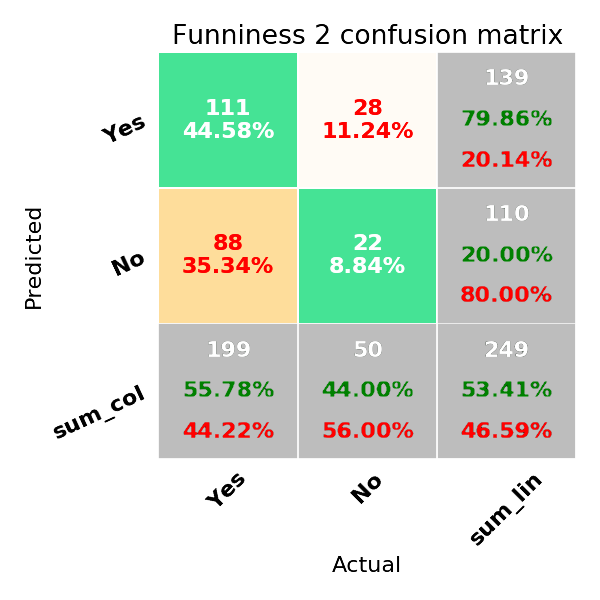
\includegraphics[width=0.9\textwidth,height=0.3\textheight,keepaspectratio]{graphics/twostageperf/funniness2}
\end{subfigure}

\begin{subfigure}[b]{0.45\textwidth}
\centering
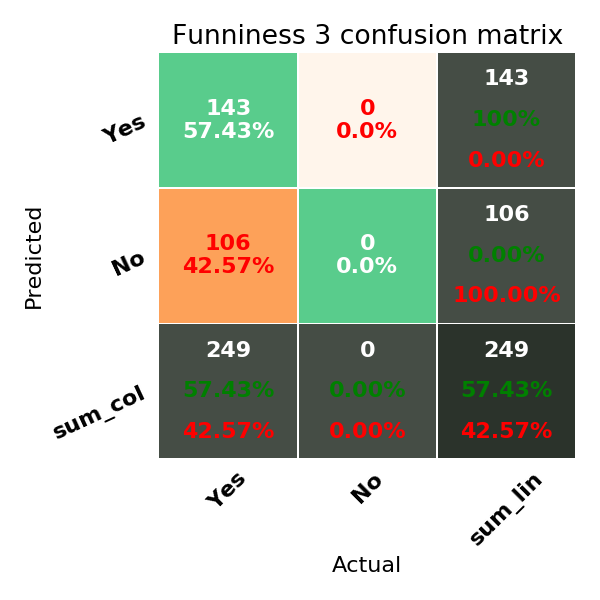
\includegraphics[width=0.9\textwidth,height=0.3\textheight,keepaspectratio]{graphics/twostageperf/funniness3}
\end{subfigure}\quad
\begin{subfigure}[b]{0.45\textwidth}
\centering
\includegraphics[width=0.9\textwidth,height=0.3\textheight,keepaspectratio]{graphics/twostageperf/funniness4}
\end{subfigure}

\begin{subfigure}[b]{0.45\textwidth}
\centering
\includegraphics[width=0.9\textwidth,height=0.3\textheight,keepaspectratio]{graphics/twostageperf/funniness5}
\end{subfigure}\quad
\begin{subfigure}[b]{0.45\textwidth}
\centering
\includegraphics[width=0.9\textwidth,height=0.3\textheight,keepaspectratio]{graphics/twostageperf/funniness6}
\end{subfigure}


\begin{subfigure}[b]{0.45\textwidth}
\centering
\includegraphics[width=0.9\textwidth,height=0.3\textheight,keepaspectratio]{graphics/twostageperf/funniness7}
\end{subfigure}


\caption{Confusion Matrices for first stage.}
\label{fig:firststageconf}

\end{figure}


\subsection{Autoencoder}

The goal of the auto encoder using the deep convolutional architecture is to reduce the dimensionality of the images, while still maintaining the important characteristics of the original cartoons. 

Comparing the reconstructed cartoon with the original cartoon reveals that the autoencoder looses important semantic information which could be crucial for understanding humor. For example the facial expressions are lost, as well as many other high frequency details. For example the native American lying on the floor is not recognizable anymore. 

These details seem to be very important for the funniness classification task and if missing cause the image data to be not more than additional noise, which is probably the reason why the two stage model with autoencoded cartoons performs worse.

\begin{figure}
	\centering
  	\includegraphics[width=1.0\textwidth]{graphics/autoencoder_original.png}
	\caption{Original Cartoons}
	\label{fig:autoencoderimageoriginal}
\end{figure}

\begin{figure}
	\centering
  	\includegraphics[width=1.0\textwidth]{graphics/autoencoder_final.png}
	\caption{Results after applying encoder and decoder}
	\label{fig:autoencoderresults}
\end{figure}

\section{Results}

The following sections show the achieved performance for each experiment of the validation
and test phase. Additionally the training runtime is also listed.


\subsection{Validation Results}

For a detailed table of validation performance of selected models, please refer to figure [\ref{fig:valperformance}]. The ELMo based model achieved on this subset the highest accuracy, while the Two Stage Model achieved the best mean Absolute Error. Both models only use the text data and discard the visual information entirely.

\begin{figure}
\begin{tabular}{|l|l|l|l|l|}
\hline
\textbf{Experiment}                                                                       & \textbf{\begin{tabular}[c]{@{}l@{}}Validation\\   MAE\end{tabular}} & \textbf{\begin{tabular}[c]{@{}l@{}}Validation\\   Accuracy\end{tabular}} & \textbf{Text} & \textbf{Visual} \\ \hline
Baseline Most Frequent                                                                    & 2.14                                                                & 25.20\%                                                                  &               &                 \\
Baseline Average                                                                          & 1.53                                                                & 13.94\%                                                                  &               &                 \\
Baseline Random                                                                           & 2.33                                                                & 13.81\%                                                                  &               &                 \\
Baseline Stratified                                                                       & 2.03                                                                & 16.62\%                                                                  &               &                 \\
Simple CNN                                                                                & 2.14                                                                & 25.20\%                                                                  &               & \cmark               \\
Transfer Learning CNN                                                                      & 1.88                                                                & 25.53\%                                                                  &               & \cmark               \\
\begin{tabular}[c]{@{}l@{}}Transfer Learning CNN (with\\   data augmentation)\end{tabular} & 1.96                                                                & 23.86\%                                                                  &               & \cmark               \\
ELMo                                                                                      & 1.81                                                                & \textbf{26.81\%}                                                                  & \cmark             &                 \\
AutoML Model with ELMo Vectors                                                            & 2                                                                   & 25.87\%                                                                  & \cmark             &                 \\
\begin{tabular}[c]{@{}l@{}}AutoML Model with TFIDF\\   Vectors\end{tabular}               & 2.05                                                                & 26.76\%                                                                  & \cmark             &                 \\
Two Stage Model                                                                           & \textbf{1.52}                                                                & 18.10\%                                                                  & \cmark             & \\
Two Stage Model with Cartoons                                                             & 1.55                                                                & 15.68\%                                                                  & \cmark             & \cmark               \\
\begin{tabular}[c]{@{}l@{}}Two Stage Model with\\   Autoencoded Cartoons\end{tabular}     & 1.62                                                                & 15.82\%                                                                  & \cmark             & \cmark               \\ \hline
\end{tabular}
\caption{Model performances on the validation set.}
\label{fig:valperformance}
\end{figure}

\subsection{Test Results}

The results at figure [\ref{fig:testperformance}] show the performance of the models for the test set. Compared to the validation set the best performing models change: The model which maximizes the accuracy measure is now using the visual data, namely the transfer learning CNN on the data augmented test set. Also the two stage model without cartoon data seems to generalize slightly better.

\begin{figure}
\begin{tabular}{|l|l|l|l|l|}
\hline
\textbf{Experiment}                                                                       & \textbf{Test MAE} & \textbf{Test Accuracy} & \textbf{Text} & \textbf{Visual} \\ \hline
Baseline Most Frequent                                                                    & 2.26              & 24.50\%                &               &                 \\
Baseline Average                                                                          & \textbf{1.57}              & 11.65\%                &               &                 \\
Baseline Random                                                                           & 2.17              & 13.65\%                &               &                 \\
Baseline Stratified                                                                       & 2.22              & 14.46\%                &               &                 \\
Simple CNN                                                                                & 2.26              & 24.50\%                &               & \cmark               \\
Transfer Learning CNN                                                                      & 1.96              & 24.90\%                &               & \cmark               \\
\begin{tabular}[c]{@{}l@{}}Transfer Learning CNN (with\\   data augmentation)\end{tabular} & 2.01              & \textbf{26.10\%}                &               & \cmark               \\
ELMo                                                                                      & 1.84              & 25.70\%                & \cmark             &                 \\
AutoML Model with ELMo Vectors                                                            & 2.12              & 24.50\%                & \cmark             &                 \\
\begin{tabular}[c]{@{}l@{}}AutoML Model with TFIDF\\   Vectors\end{tabular}               & 2.23              & 24.90\%                & \cmark             &                 \\
Two Stage Model                                                                           & 1.6               & 18.80\%                & \cmark             &                 \\
Two Stage Model with Cartoons                                                             & \textbf{1.57}              & 16.06\%                & \cmark             & \cmark               \\
\begin{tabular}[c]{@{}l@{}}Two Stage Model with\\   Autoencoded Cartoons\end{tabular}     & 1.58              & 14.46\%                &\cmark             & \cmark              \\
\hline
\end{tabular}
\caption{Model performances on the test set.}
\label{fig:testperformance}
\end{figure}

\subsection{Training Duration}

Figure [\ref{trainingruntime}] shows the training durations of each experiment. A general trend, is that the text based models (ELMo, Two Stage Model) train significantly faster than the visual based models (Simple CNN, Transfer Learning CNN, Two Stage Model with Cartoons). This can be explained by the size of the input vector for the neural network. The data for the text representation is denser compared to the representation of images.

\begin{figure}
\centering
\begin{tabular}{|l|l|} 
\hline
\textbf{Experiment}                                    & \textbf{Train Duration}  \\ 
\hline
Baseline Most Frequent                        & \textless{}1s   \\
Baseline Average                              & \textless{}1s   \\
Baseline Random                               & \textless{}1s   \\
Baseline Stratified                           & \textless{}1s   \\
Simple CNN                                    & 7m 50s          \\
Tranfer Learning CNN                          & 15m 45s         \\
Tranfer Learning CNN (with data augmentation) & 9m 52s          \\
ELMo                                          & 4m 39s          \\
AutoML Model with ELMo Vectors                & 29m 7s          \\
AutoML Model with TFIDF Vectors               & 24m 20s         \\
Two Stage Model                               & 8m 42s          \\
Two Stage Model with Cartoons                 & 39m 42s         \\
Autoencoder                                   & 32m 34s         \\
Two Stage Model with Autoencoded Cartoons     & 15m 23s         \\
\hline
\end{tabular}
\caption{Training runtime of each experiment}
\label{trainingruntime}
\end{figure}



\section{Discussion}
Seiten: 2

Discussion der Ergebnisse der Evaluation.

\chapter {Conclusion}

In general no model really learns to generalize the humor of Gary Larson. There has been no significant improvement compared to the baselines. Further research could reveal significant insights on how human humor works.

Potential causes can not be attributed to exactly one issue. One reason is most certainly, that the problem space is not sufficiently grasped by the dataset. As most deep learning datasets are many order of magnitudes larger, while the task at hand is arguably easier (For example: CIFAR 10 dataset \cite{dogsvscats}) than humor classification. Current techniques of transfer learning are not sufficient to solve this issue. Most certainly once more sophisticated transfer learning techniques have been established, solving this problem could be more feasible. 

One could also argue that the problem itself is flawed. Letting a human rate a
cartoon is very subjective and likely depends on many factors. For example: Current mood, whether the person has already seen the cartoon, time of day and also the exact reason for performing the annotation. It could be that these factors outweigh the true humor, which makes it impossible to reproduce the original ratings. To answer this question an additional experiment could be performed: After some time after the initial ratings were performed, the same person rates the cartoons again. If the ratings are not reproducible by the same annotator, then it seems to be impossible for a deep learning based model.


%\chapter{Introduction}
%\todo{Enter your text here.}

%\chapter{Additional Chapter}
%\todo{Enter your text here.}

\backmatter

% Use an optional list of figures.
\listoffigures % Starred version, i.e., \listoffigures*, removes the toc entry.

% Use an optional list of tables.
% \cleardoublepage % Start list of tables on the next empty right hand page.

% \listoftables % Starred version, i.e., \listoftables*, removes the toc entry.

% Use an optional list of alogrithms.
% \listofalgorithms
% \addcontentsline{toc}{chapter}{List of Algorithms}

% Add an index.
% \printindex

% Add a glossary.
% \printglossaries

% Add a bibliography.
\bibliographystyle{abbrv}
\bibliography{citations}

\end{document}